%-------------------------------------------------------------------------------
%
% TUM Dissertation Template
%
% For usage instructions see README.md
%
% Authors:
%   Andre Richter, andre.richter@tum.de
%   Michael Vonbun, michael.vonbun@tum.de
%   Christian Herber, christian.herber@tum.de
%   Stefan Wallentowitz, stefan.wallentowitz@tum.de
%
%-------------------------------------------------------------------------------
\documentclass[%
  % layouttitlepage,            % layout help rules (to see if you need
  %                             % some extra vspace in your title etc.)
  % headings = standardclasses, % serif fonts for headings
  % headings = big,             % If you use serif fonts for headings (above option
  %                             % uncommmented), uncomment this one to get smaller
  %                             % headings
  % sansseriftitlepage,         % sans serif title page
  % notocintoc,                 % do not add toc to toc itself
]{tumDiss}
\usepackage[utf8]{inputenc}



%-------------------------------------------------------------------------------
% Binding correction for the title page.
% WARNING: ONLY NEEDED FOR THE PRINT VERSION!
%
% After printing and binding, the left part of the titlepage may lose
% significant space, for example due to overlap from glue binding.
% You can increase the left margin of the title page with this option.
% This value of 8mm was measured for glue binding a thesis that was printed by
% the TUM Fachschaft EI and ~140 pages.
%-------------------------------------------------------------------------------
% \titlepagebindingcor{8mm}

%-------------------------------------------------------------------------------
% Binding correction for everything else.
% Does not affect titlePageBindingCor!
%
% WARNING: THIS OPTION CAN SHAKE UP YOUR CURRENT LAYOUT.
% If you want to use it, it is best to work with it from the very start. Adding
% it when finishing your dissertation might get you into trouble.
%
% Search http://texdoc.net/texmf-dist/doc/latex/koma-script/scrguien.pdf for
% "BCOR" for further reading.
%-------------------------------------------------------------------------------
% \KOMAoptions{BCOR=3mm}



%-------------------------------------------------------------------------------
% Faculty
%-------------------------------------------------------------------------------
\faculty{Fakultät für Informatik}

%-------------------------------------------------------------------------------
% Degree
%-------------------------------------------------------------------------------
\degree{Doktors der Naturwissenschaften (Dr. rer. nat.)}

%-------------------------------------------------------------------------------
% Title
%
% IMPORTANT:
%
% You must add manual line breaks here. If you don't, you'll get uneven spacing
% between the lines.
% YOU ALSO NEED THE BREAK AT THE LAST LINE.
%-------------------------------------------------------------------------------
\title{%
  Uncertainty Estimation\\ 
  for I.I.D., Graph, and Sequential Data\\
}
% \subtitle{That is extended by using an additional subtitle}

%-------------------------------------------------------------------------------
% People
%-------------------------------------------------------------------------------
\author{Bertrand Charpentier}
\vorsitz{Prof. Dr.- Vorname Nachname}
\erstpruef{Prof. Dr.- Stephan Günnemann}

% Use this one for a TUM professor
% \zweitpruef{Prof. Dr.-Ing. Vorname Nachname}

% Or this one for an external professor
\zweitpruef[Technische Universität Berlin]{Prof. Dr.-Ing. Vorname Nachname}

% Optionally, add a third examiner
%\drittpruef[RWTH Aachen]{Prof. Dr.-Ing. Max Mustermann}

%-------------------------------------------------------------------------------
% Hand in date
%
% This is the date of your personal hand-in at the TUM doctoral office.
%-------------------------------------------------------------------------------
\date{01.01.2016}

%-------------------------------------------------------------------------------
% Accepted date
%
% You can set this after your thesis was accepted. For handing in,
% it is not needed (at least for the Electrical Engineering faculty).
%-------------------------------------------------------------------------------
\dateaccepted{10.05.2016}



%-------------------------------------------------------------------------------
% Change language, e.g. to german
%-------------------------------------------------------------------------------
% \usepackage[ngerman]{babel}

%-------------------------------------------------------------------------------
% Compatibility issues
%-------------------------------------------------------------------------------
% If you need pstricks, load it here before everything else.
% Otherwise, tikz patterns won't work
%\usepackage{pstricks}

%-------------------------------------------------------------------------------
% Suggested standard packets are included here
%-------------------------------------------------------------------------------
% Loading scrhack fixes:
%   (1) KOMA-Script incompatible macros used in listings package.
%   (2) Inconsistent anchors in hyperref.
\usepackage{scrhack}


% figure inclusion
\usepackage{amsthm}
%\usepackage[
%  caption = false,
%  font    = footnotesize
%]{subfig}
\usepackage{graphicx}
\usepackage{pgfplots}
\usepackage{pgfplotstable}
\usepackage[numbers]{natbib}
\tikzset{>=stealth}
\usetikzlibrary{patterns}
\usetikzlibrary{pgfplots.statistics}

\usepackage{tocloft}
\newlength\mylen
\renewcommand\cftpartpresnum{Part~}
\settowidth\mylen{\bfseries\cftpartpresnum\cftpartaftersnum}
\addtolength\cftpartnumwidth{\mylen}

% code block insertion
\usepackage{moreverb}
\usepackage{listings}

% math and equations
\usepackage{amsmath}
\usepackage{amssymb}
\usepackage{amsfonts}
\usepackage{upgreek}

% enumeration
\usepackage{enumerate}

\usepackage{booktabs} % For formal tables
\usepackage{xspace}
\usepackage{mathtools, cuted}
\usepackage{subcaption}
\usepackage{graphicx,caption}
\usepackage{wrapfig}
%\usepackage{arydshln}
\usepackage{floatflt}
\usepackage[ruled,vlined]{algorithm2e}
\usepackage{bm}
\usepackage{pgf}
\usepackage{makecell}
\usepackage{rotating, multirow}
\usepackage{tikz}
\usetikzlibrary{positioning}
\usetikzlibrary{backgrounds,matrix,patterns}
\usetikzlibrary{decorations.pathmorphing, patterns}
\definecolor{color0}{RGB}{220, 38, 127}
\definecolor{color1}{RGB}{100, 143, 255}
\definecolor{color2}{RGB}{254, 97, 0}
\definecolor{color3}{RGB}{120, 94, 240}
\definecolor{color4}{RGB}{255, 176, 0}

% Source code with highlighting
\usepackage{listings}
\lstset{
  basicstyle       = \footnotesize,
  captionpos       = b,
  tabsize          = 4,
  commentstyle     = \color{TUMGreen},
  keywordstyle     = \color{TUMBlue},
  stringstyle      = \color{TUMOrange},
  otherkeywords    = {
    uint64_t,
    uint32_t,
    uint16_t,
    uint8_t,
    u64,
    u32,
    u16,
    u8,
    inline
  },
  numbers          = left,
  xleftmargin      = 7ex,
  aboveskip        = 4ex,
  abovecaptionskip = 2ex,
}

% Support for siunitx
\usepackage{siunitx}
\sisetup{
  exponent-product = \cdot,
  output-product   = \cdot,
  per-mode         = symbol-or-fraction,
  quotient-mode    = fraction,
  binary-units     = true
}

% No widows and orphans
\usepackage[all]{nowidow}

% dummy text
\usepackage{lipsum}

% hyperlinks
% according to its documentation, hyperref should be loaded last
% a list of packages that should be loaded after hyperref can be found at
% https://tex.stackexchange.com/questions/1863/which-packages-should-be-loaded-after-hyperref-instead-of-before
\usepackage{url}
\usepackage[
  hidelinks,
  bookmarksnumbered
]{hyperref}

% If hyperref is used, references to tables and figures link to their captions
% and not the actual tables or figures. This is especially unwanted for figures,
% because their captions are below the figure so that clicking on a link just
% shows the captions and the figure is invisible.
%
% Using the caption package fixes this behaviour.
\usepackage{caption}

% glossary functionality
% loading glossaries after hyperref adds hyperlings to acronyms and glossary
% entries
\usepackage[
  toc,
  acronym,
  style = long
]{glossaries}
\makeglossaries

%-------------------------------------------------------------------------------
% Include custom packages here
%-------------------------------------------------------------------------------

% \usepackage{}


%-------------------------------------------------------------------------------
% TUM CI colors for PGF
%-------------------------------------------------------------------------------
\definecolor{grey60} {RGB} {102, 102, 102} % 60% grey

%-------------------------------------------------------------------------------
% Default values for pgfplots
%-------------------------------------------------------------------------------
\newcommand{\figureHeight}{0.5625} %% 16:9
\pgfplotsset{
  compat           = 1.13,
  grid             = major,
  enlarge x limits = 0,
  cycle list name  = tum,
  major grid style = {dotted},
  minor grid style = {dotted},
  legend style     = {
    at     = {(0.98,0.96)},
    anchor = north east,
  },
  width            = \hsize * 0.9,
  height           = \hsize * 0.9 * \figureHeight,
}

%-------------------------------------------------------------------------------
% Correct bad hyphenation here
%-------------------------------------------------------------------------------
\hyphenation{op-tical net-works semi-conduc-tor}

%-------------------------------------------------------------------------------
% Acronyms (will be sorted alphabetically)
%-------------------------------------------------------------------------------
\newacronym{cpu}{CPU}{Central Processing Unit}
\glsadd{cpu}

\newacronym{pci}{PCI}{Peripheral Component Interconnect}
\glsadd{pci}

\newacronym{pcie}{PCIe}{Peripheral Component Interconnect Express}
\glsadd{pcie}

\newacronym{mmu}{MMU}{Memory Management Unit}
\glsadd{mmu}



%-------------------------------------------------------------------------------
% Actual document starts here
%-------------------------------------------------------------------------------
\begin{document}
\frontmatter
\maketitle


\chapter*{Abstract}
\addcontentsline{toc}{chapter}{\protect Abstract}%

Uncertainty estimation is a crucial to build reliable machine learning models for both \emph{practical} and \emph{theoretical} reasons. While uncertainty estimation is expected to bring \emph{trust}, \emph{safety}, \emph{fairness} and facilitate \emph{maintenance} in real-world applications, uncertainty estimation is also highly required to represent the real physical world which is inherently \emph{non-deterministic} and \emph{partially observable}. 

Further, machine learning models are confronted with various types of input data (e.g. tabular, images, graph data, sequential data) and output data (classes, real values, counts, time events) which are either \emph{independent} or \emph{non-independent}. While the independence assumption is convenient to represent many data types, the non-independence assumption is particularly useful to represent complex data types with network effect or time effect.

In this thesis, we look at uncertainty estimation for both independent and non-independent data. To this end, we look at three main points: \textbf{(1)} We propose \emph{desiderata} capturing the desired behavior of uncertainty estimation. These desiderata cover both aleatoric and epistemic uncertainty in the presence of (adversarial) perturbations, network effects, or time effects. \textbf{(2)} We propose a large family of new Bayesian \emph{models} which provide uncertainty estimates at a low practical cost. These models demonstrate strong empirical performance and have theoretical guarantees. \textbf{(3)} We propose extensive \emph{experimental setups} to evaluate uncertainty estimates for practical tasks. These experimental setups cover correct/wrong prediction, detection, OOD detection, dataset shifts, and calibration metrics in the presence of (adversarial) perturbations, network effects, or time effects.
\\

\chapter*{Zusammenfassung}
\addcontentsline{toc}{chapter}{\protect Zusammenfassung}%

This is the german abstract.
\chapter*{Acknowledgements}
\addcontentsline{toc}{chapter}{\protect Acknowledgements}%



I would first like to thank my supervisor Prof.~Stephan Günnemann. I feel incredibly lucky for the opportunity to pursue a Ph.D. under your guidance. Thank you for showing me how to become a better researcher, teacher, presenter, and supervisor. I enjoyed our brainstorming sessions where you always provided helpful and precise feedback. Thank you for your understanding and great support which was always motivating to achieve great work.

I am very grateful to all DAML group. I could not have imagined a better environment for my Ph.D. study. I would like to thank everyone in the group for their readiness to help, discuss ideas, and share research progress. It was a lot of fun during and outside working hours. I would like to particularly thank all my colleagues, collaborators, and co-authors I had the chance to work with at the Technical University of Munich. Thank you Simon Geisler, Anna-Kathrin Kopetzki, Tom Wollshläger, and Nicholas Gao. Thank you also Marin Biloš for your support, help, and your great sense of humor. It was a lot of fun to share our office. Special thanks to Daniel Zügner for all your support and openness. Beyond all the great research collaborations, I would like to thank you for all the friendly discussions and advice.

While pursuing my Ph.D., I had the chance to work with bright, curious, and motivated students. Thank you Oliver, Maximilian, Daniel, Johannes, Sascha, Igor, Franz, Raphael, Niklas, Stephan, Simon, Sven, Chenxiang, Xun, Morgane, and John.

I am very grateful to Prof. Mykel Kochenderfer from Stanford University for hosting me during my research stay. I would like to thank everyone from SISL lab with special thanks to Ransalu Senanayake. You always make me feel welcome and provided me with great advice during my stay.

I am also very grateful to the members of the Twitter Cortex team for your warm welcome and support despite the intense time at the company. I would like to particularly thank Nils Hammerla, Emanuele Rossi, Francesco Di Giovianni, and Prof. Michael Bronstein for the great discussions and research collaborations.

I would also like to express my very profound gratitude to my family, my friends, and my partner for providing me with continuous encouragement, joy, and happiness throughout these years. I am particularly thankful to my parents who provided me with unconditional support. I love you.

This thesis is also dedicated to my beloved grandfather Alain, godfather Bertrand, and cousin Quentin who passed away. Thank you for all the time that I could share with you. You remain a great source of inspiration for me.



%-------------------------------------------------------------------------------
\tableofcontents
%\listoffigures
%\listoftables
%\printglossary[type=\acronymtype, nonumberlist]


%-------------------------------------------------------------------------------
\mainmatter
\part{Introduction}
\chapter{Introduction}
\label{chap:introduction}

Artificical Intelligence (AI) consists of the intelligence demonstrated by machines in contrast with intelligence demonstrated by humans or animals.
AI includes both Machine Learning (ML) which consists in the study of computer programs which automatically learn from experience \citep{Mitchell97}, and Deep Learning (DL) which is a subfield of ML and can be defined as models which hierarchically learn complex representations based on simpler ones \citep{GoodBengCour16}.
AI is a very important technology with high potential economical and ethical impact. 

Economically, AI has a high momentum. Indeed, 48\% of companies claim that they use AI \cite{ai-market-oreilly} and 83\% companies have AI is their priority \cite{ai-market-forbes}. Overall, the market value of AI is \$136 billion in 2022 \cite{ai-market} and had a Compound Annual Growth Rate (CAGR) of 38.5\% between 2022-2030 \cite{ai-market}, thus indicating a very fast growth.
Hence, AI founds many applications in science and industry. 
Industry applications include e.g. agriculture (e.g. Cropin, Iron Ox, FarmWise), manufacturing (e.g. Exotec, Bright Machines, Fieldbox), automotive industry (e.g. Tesla, Waymo), medicine (e.g. Exscientia, Valence Discovery, Radium), construction (Procore Technologies, OpenSpace), finance (e.g. Affirm, Kreditech, Kayrros), education (e.g. Duolingo, Age of Learning), or even for art (e.g. Bytedance, OpenAI).
Scientific applications include e.g. physics (e.g. \cite{gao2022abinitio}), chemistry (e.g. \cite{huang2021abinitio}), biology (e.g. \cite{hetzel2022predicting}), or even math (e.g. \cite{cobbe2021math}).
Hence, AI have shown to be applicable in various data types (e.g. images, tabular, text, graphs) and at various scales from very small (e.g. molecules) to very large systems (e.g. social networks).

Ethically, AI systems demonstrate multiple important concerns.
It does not guarantee a safe behavior and can create accidents \cite{amodei2019problems}.
It does not provide clear explanations for its predictions or provide unreliable explanations \cite{overview-interpretable-ml,interpretable-ml, krishnan2020against}.
It might be racist and discriminate minorities \cite{mehrabi2019fairness}.
It can partially replace human jobs by stealing human creations which leaves the question of intellectual property unclear \cite{moerland2022intellectual, gervais2020intellectual}.
Finally, it might have goals which are not aligned with human goals. This is particularly problematic when AI systems achieve a super-intelligence \cite{bostrom2014superintelligence} which is realistic in many task where AI systems are already better than humans \cite{firestone2020performance}.

The fast AI economic growth and the multiple AI ethical concerns urge the development of reliable AI models which is the main subject of this thesis.

\section{Why do we need uncertainty ?}

Uncertainty estimation (a.k.a. uncertainty quantification) consists in evaluating the confidence of models in their predictions. This task is crucial for both practical and theoretical reasons summarized in Fig.~\ref{fig:uncertainty_reasons}.

\begin{figure}[ht!]
    \centering
    \begin{subfigure}[t]{1. \columnwidth}
        \centering
        $\vcenter{\hbox{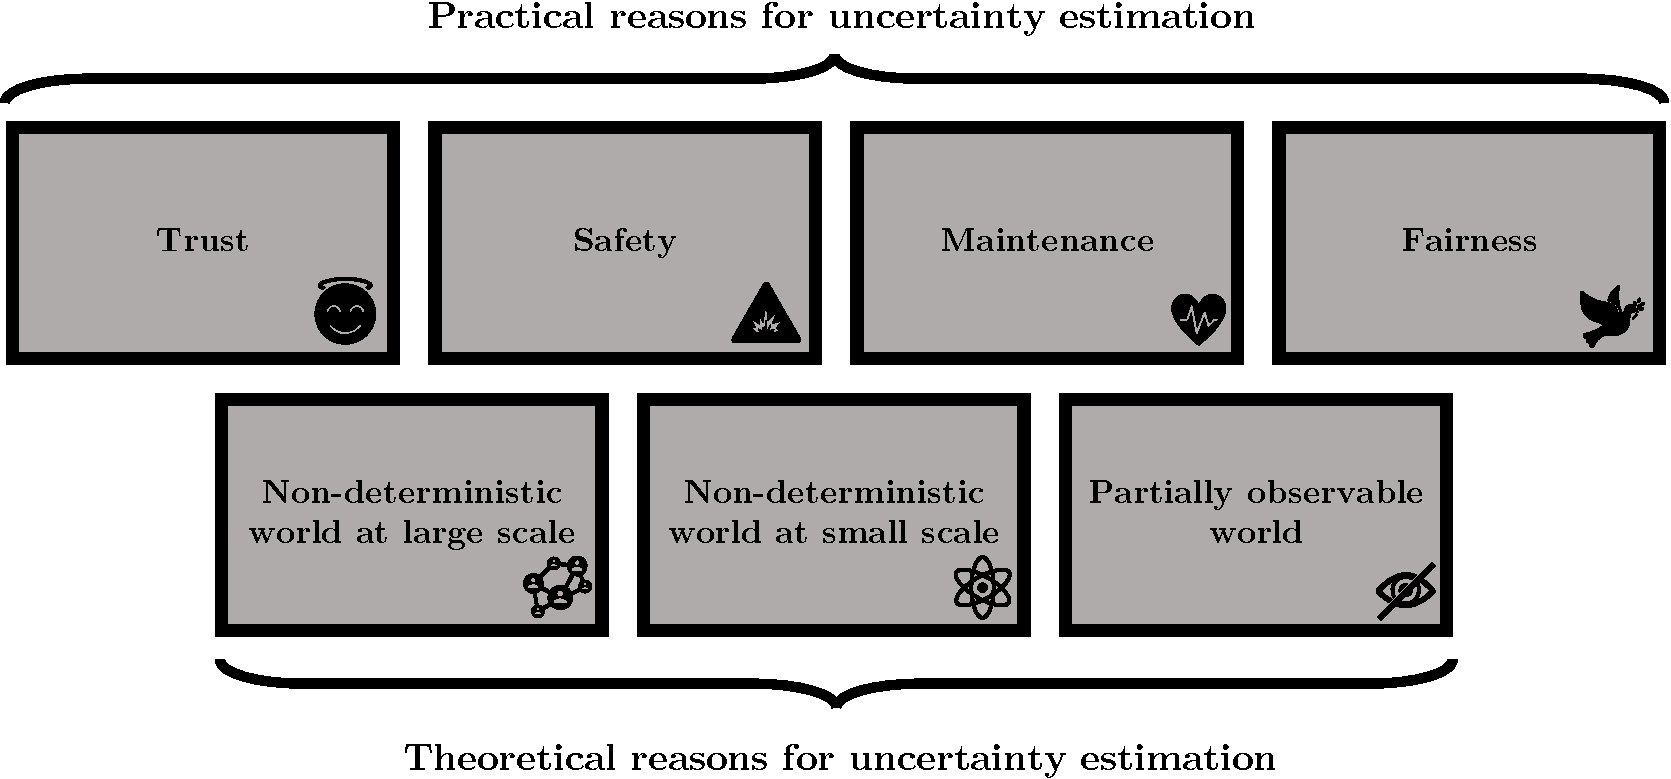
\includegraphics[width=0.9 \textwidth]{resources/uncertainty_reasons.pdf}}}$
    \end{subfigure}%
    \caption{Overview of the \emph{practical} and \emph{theoretical} reasons for uncertainty estimation.}
    \label{fig:uncertainty_reasons}
	% \vspace{-.5cm}
\end{figure}

\paragraph*{Practical reasons.} The Dunning-Kruger effect \cite{dunning-kruger} describes a psychological cognitive bias in which people lacking knowledge in a particular domain overestimate their abilities. Interestingly, this phenomenon also applies to machine learning models. Traditional neural networks show overconfident predictions, in particular on data that is different from the data seen during training \cite{overconfident-relu}. The illusion of knowledge of machine learning models highly impacts the reliability of such  models  in  safety-critical  domains.
First, it affects the \emph{trust} in ML model predictions. Ideally, we expect ML models to be confident when predicting correctly and uncertain when predicting wrongly. 
Second, it affects the \emph{safety} of ML predictions in unfamiliar situations. Ideally, we expect ML models to flag predictions on unknown domains corresponding to anomaly detection.
Third, it affects the \emph{maintenance} of ML models. Ideally, we expect ML models to become more uncertain when the testing data has drifted away from the training data, thus indicating the need of retraining the model. This is particularly important in application where ML models need to explore and learn all life-long.
Finally, it affects the \emph{fairness} of ML models. Ideally, we expect ML models to provide calibrated predictions on all input regions including underrepresented data.
A summary of the practical reasons and their associated use cases is given in table \bc{Do table}.

\paragraph*{Theoretical reasons.} ML models aim at precisely representing the flow of information in the world which is inherently uncertain.
The world is \emph{non-deterministic at a large scale}. Indeed, uncertainty emerges when small individual events contribute to macro phenomena like GDP growth, micro phenomena like the growth rate of firms, and non-economic events like war and climate change \cite{macro-micro-uncertainty}.
The world is \emph{non-deterministic at a small scale}. Indeed, the uncertainty principle in (quantum) physics implies that it is in general not possible to predict the value of a particle quantity (like position and speed) with arbitrary certainty, even if all initial conditions are specified \cite{hilgevoord2016heisenberg}.
The world is only \emph{partially observable}. Indeed, agents like humans or robots have to deal with incomplete information on the environment in which they evolve \cite{kaelbling1998pomdp}. At the extreme, since the speed of information is limited by the speed of light, accessible information is restricted to the observable world, thus making the world inherently uncertainty for any agent \cite{ord2021universe}.
A summary of the theoretical reasons is given in table \bc{table}.


\paragraph*{} All these reasons underline the need of accurate uncertainty estimation methods in ML. 
Specifically, a reliable ML model should provide high-quality estimates of \emph{aleatoric} and \emph{epistemic} uncertainty \citep{uncertainty-deep-learning}.
The aleatoric uncertainty allows a model to account for the irreducible data uncertainty (e.g. the inherent sensor noise, or the inherent environment stochasticity).
The epistemic uncertainty allows a model to account for its lack of knowledge about unseen data regions (e.g. testing data differs significantly from training data).
Aleatoric and epistemic uncertainty levels can eventually be combined into an overall \emph{predictive} uncertainty \citep{uncertainty-deep-learning}. Hence, this thesis studies the usage of different types of uncertainty for ML methods.

\section{Why do we need independent and non-independent data ?}

In this thesis, we consider ML models which process input data to accurately predict output targets. 
More specifically, we expect ML models to be able to process \emph{any type of input data} (e.g. tabular, images, graph or time series) to predict \emph{any type of output data} (e.g. classes, continuous values, counts).
To this end, \emph{independence} and \emph{non-independence} are key assumptions to create \emph{practical} and \emph{accurate} models which precisely describe the real-world. 

\begin{figure}[ht!]
    \centering
    \begin{subfigure}[t]{0.245 \columnwidth}
        \centering
        $\vcenter{\hbox{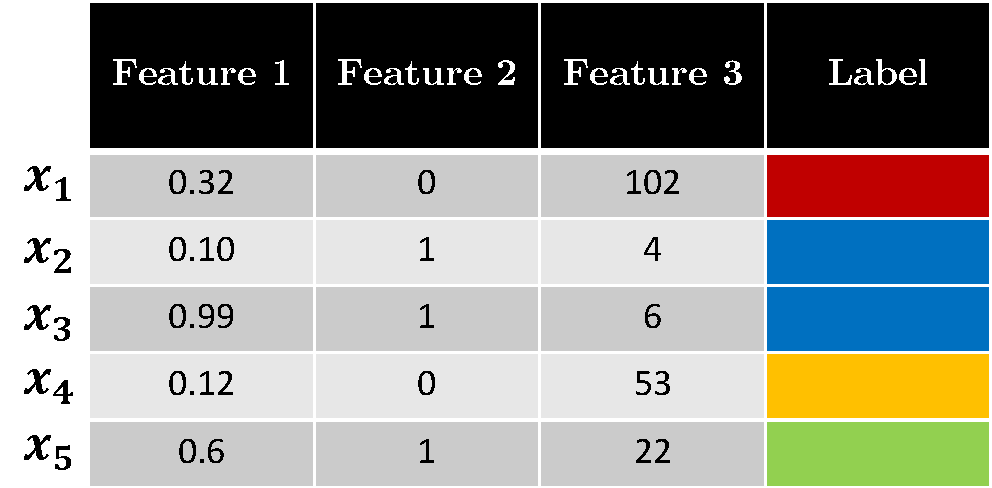
\includegraphics[width=0.9 \textwidth]{resources/tabular-cropped.pdf}}}$
         \caption{Tabular data}
         \label{fig:tabular_data}
    \end{subfigure}%
    \begin{subfigure}[t]{0.245\columnwidth}
        \centering
        $\vcenter{\hbox{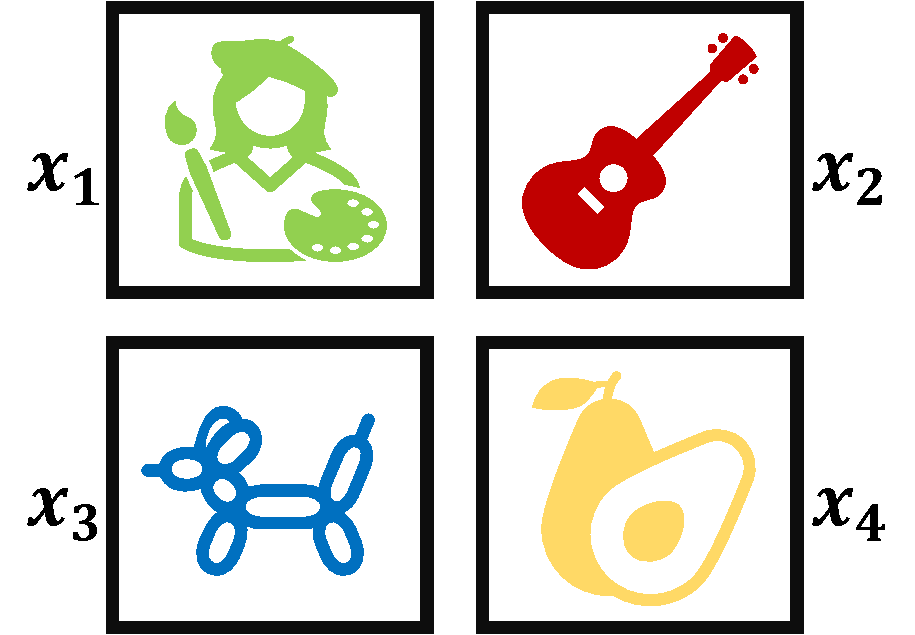
\includegraphics[width=0.9 \textwidth]{resources/image-cropped.pdf}}}$
        \caption{Image data}
        \label{fig:image_data}
    \end{subfigure}%
    \begin{subfigure}[t]{0.245 \columnwidth}
        \centering
        $\vcenter{\hbox{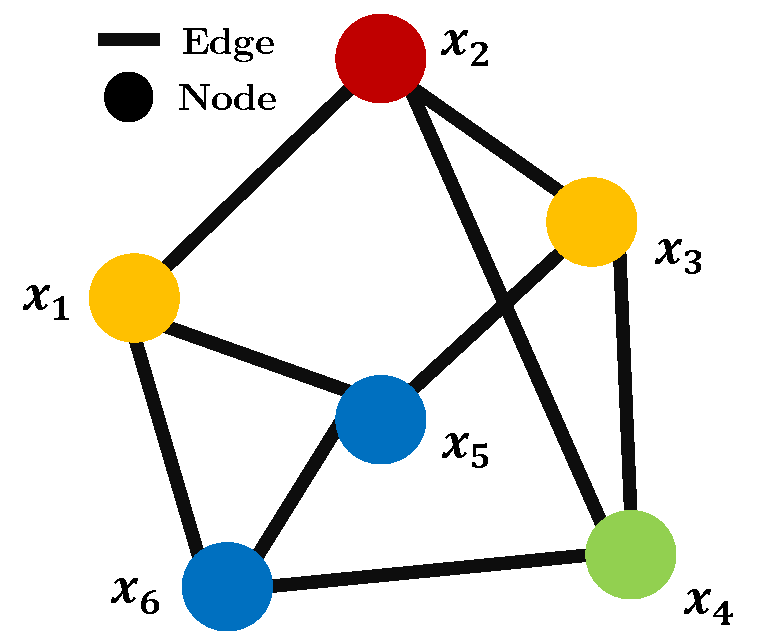
\includegraphics[width=0.9 \textwidth]{resources/graph-cropped.pdf}}}$
         \caption{Graph data}
         \label{fig:graph_data}
    \end{subfigure}%
    \begin{subfigure}[t]{0.245\columnwidth}
        \centering
        $\vcenter{\hbox{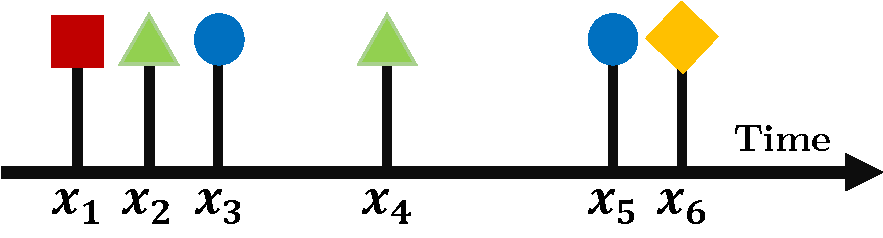
\includegraphics[width=0.9 \textwidth]{resources/sequential-cropped.pdf}}}$
        \caption{Sequential data}
        \label{fig:sequential_data}
    \end{subfigure}%
    \caption{Overview of different data types covering independent $\x_i$ inputs like tabular and image data, and dependent $\x_i$ inputs like graph node and sequential time events.}
	% \vspace{-.5cm}
\end{figure}

\paragraph*{Independent Data.} The independence assumption means that different data samples are not connected in any way. In other words, the knowledge of one data sample does not bring any information on another data sample.
The independence assumption is particularly useful when representing tabular data \cite{raschka2022chronology} (e.g. a group of unrelated persons for a medicine trial, defects on multiple different devices) or image data \cite{lu2020survey, litjens2017survey} (e.g. disease detection on medical images of different patients, object detection in different self-driving cars or robots). Visualizations of such data are represented in Fig.~\ref{fig:tabular_data} and Fig.~\ref{fig:image_data}.
In this case, representing the interaction between data samples does not bring much information to perform the predictions.
Hence, the key advantage of the independence assumption is that it allows mathematical factorization for practical modelling simplifications \citep{bishop} without important information loss.

\paragraph*{Non-Independent Data.} The non-independence assumption means that different data samples might be connected in some way. In other words, observing a data sample gives some information on the value of another data sample.
The non-independence assumption is particularly useful when representing graph data \cite{GNNBook2022} (e.g. social networks, citation networks) or sequential data \cite{shchur2021review, Dietterich2002Machine} (e.g. financial time series, interaction history of a user). Visualizations of such data are represented in Fig.~\ref{fig:graph_data} and Fig.~\ref{fig:sequential_data}.
In this case, neighboring nodes of a graph are expected to share important information and past events are expected to give important information on future events.
Hence, the key advantage of the non-independence assumption is that it retains the information contained in graph and sequential interactions to model the world more precisely.

\paragraph*{} Beyond the \emph{(non-)independence assumption}, another common assumption in ML is that data are \emph{identically distributed}. 
This assumption assumes that all input data comes from the same data distribution which also has strong limitations related to the reasons motivating the usage of uncertainty estimates for ML predictions.
While the training data are assumed to come from the same data distribution, the testing data might come from different distributions and suffer from \emph{Distribution Shifts} \cite{rabanser2019shift, dataset-shift}. 
Indeed, the testing data might come from the \emph{In-Distribution (ID)} similar to the training data, or a \emph{Out-Of-Distribution (OOD)} which could be any distribution different from the training distribution \cite{ood-detection-survey, shen2021ood}.
This scenario frequently happens in \emph{safety} and \emph{maintenance} use-cases where the data distribution observed by the model continuously drifts at testing time. 

Hence, this thesis acknowledges the limitation of the standard \emph{independent and identically distributed (i.i.d.)} assumptions.
To this end, this thesis studies the application of uncertainty estimation to independent and non-independent data.

\section{Contributions and outline}

This thesis studies the application of uncertainty estimation for independent and non-independent data via three main components:
\begin{itemize}
    \item Explicit \emph{desiderata} capturing the desired behavior of uncertainty estimation.
    \item Accurate \emph{models} for uncertainty estimation with low practical overhead.
    \item Practical \emph{experimental setup} evaluating uncertainty estimation in real-world applications including worst-case scenarios.
\end{itemize} 

To this end, we start by establishing the background knowledge about uncertainty estimation in Chapter~\ref{chap:background}.

In Part~\ref{part:independent_data}, we present a study of uncertainty estimation for \emph{independent data}: 
In Chapter~\ref{chap:classification}, we construct a new Bayesian model for uncertainty estimation for classification called \PostNet{} (\PostNetacro{}). \PostNetacro{} requires a \emph{single-forward pass}, does need \emph{no OOD data during training}, and adapt to \emph{many core architectures}.
In Chapter~\ref{chap:regression}, we construct a new Bayesian model for uncertainty estimation for regression called \NatPN{} (\NatPNacro{}). Beyond regression, \NatPNacro{} applies to a \emph{large variety of supervised tasks} (incl. classification and count prediction) with \emph{very low computational overhead}.
In Chapter~\ref{chap:robustness}, we present the first study of the robustness of uncertainty models in the worst-case scenario of adversarial attacks. We show that uncertainty estimates of an important family of single-forward pass models are \emph{not robust} for many important real-world tasks (incl. correct/wrong prediction detection, adversarial examples detection, and ID/OOD detection). Further, we explore first approaches methods to improve uncertainty robustness by using \emph{adversarial training} and \emph{randomized smoothing}. 

In Part~\ref{part:non_independent_data}, we present a study of uncertainty estimation for \emph{non-independent data}:
In Chapter~\ref{chap:graph_data}, we present the first framework for uncertainty estimation for node classification on graph data. This framework proposes explicit desiderata, a new Bayesian model, and an exhaustive evaluation setup which cover aleatoric and epistemic uncertainty estimation \emph{without} and \emph{with network effects}.
In Chapter~\ref{chap:sequential_data}, we present new models for uncertainty estimation in sequential data with asynchronous time events. The two proposed models are able of accurate \emph{event types} and \emph{event time} predictions while capturing \emph{uncertainty with rich temporal evolution}.
In Chapter~\ref{chap:reinforcement_learning}, we present the first framework to disentangle aleatoric and epistemic uncertainty estimation in reinforcement learning. This framework proposes explicit desiderata, four models inspired from supervised learning, and a detailed experimental setup which cover aleatoric and epistemic uncertainty estimation at both \emph{training time} and \emph{testing time}.

In Part~\ref{part:conclusion}, we present a retrospective on the evolution of the research field since our first study (see Chapter~\ref{chap:retrospective}) and a conclusion including open questions as suggestion to future research directions (see Chapter~\ref{chap:conclusion}).

\begin{table}
    \caption{List of own publications that this thesis is based on. Code and datasets for the respective publications are available at \texttt{www.cs.cit.tum.de/daml/[project]}.}
    \vspace{2mm}
    \label{tab:publications}
    \begin{adjustbox}{max width=\textwidth}
    \begin{tabular}{lllll}
      {Ch.} & {Ref.} & {Title} & {Conference} & {Repository}\\
      \midrule
      \ref{chap:classification} & \cite{charpentier2020} & \makecell[l]{Posterior network: Uncertainty estimation without\\ ood samples via density-based pseudo-counts} & NeurIPS 2020 & \texttt{/postnet/}\\
      \ref{chap:regression} & \cite{NatPN2021} & \makecell[l]{Natural posterior network: Deep bayesian predictive\\ uncertainty for exponential family distributions.} & ICLR 2021 & \texttt{/natpn/}\\
      \ref{chap:robustness} & \cite{robustness-uncertainty-dirichlet} & \makecell[l]{Evaluating robustness of predictive uncertainty estimation:\\ Are dirichlet-based models reliable?} & ICML 2020 & \texttt{/dbu-robustness/}\\
      \ref{chap:graph_data} & \cite{graph-postnet} & \makecell[l]{Graph posterior network: Bayesian predictive uncertainty\\ for node classification.} & NeurIPS 2021 & \texttt{/graph-postnet/}\\
      \ref{chap:sequential_data} & \cite{uceloss} & \makecell[l]{Uncertainty on asynchronous time event prediction} & NeurIPS 2019 & \texttt{/uncertainty-event-prediction/}\\
      \ref{chap:reinforcement_learning} & \cite{charpentier2022uncertainty-rl} & \makecell[l]{Disentangling epistemic and aleatoric uncertainty\\ in reinforcement learning} & DFUQ - ICML 2022 & \texttt{/aleatoric-epistemic-uncertainty-rl/}\\
    \end{tabular}
    \end{adjustbox}
\end{table}

\section{Own publications}

The content of Chapters \ref{chap:classification} to \ref{chap:reinforcement_learning} is mostly based on papers previously published at international peer-reviewed conferences. We list these papers in Table~\ref{tab:publications}.
We also provide the full list of publications that the author was involved in during the PhD studies below. These publications focus on three main topics: \emph{uncertainty estimation} (incl. bayesian models, energy-based models and robustness), \emph{structure learning} (incl. hierarchical and directed acyclic graphs), and \emph{efficient ML} (incl. pruning methods and sparse neural networks).

\renewcommand{\bibsection}{}
\documentclass{article}
\usepackage[numbers]{natbib}
\begin{document}
\nocite{charpentier2020}
\nocite{NatPN2021}
\nocite{robustness-uncertainty-dirichlet}
\nocite{graph-postnet}
\nocite{uceloss}
\nocite{ood_ebm}
\nocite{charpentier2019tsd}
\nocite{bonald2020scikitnetwork}
\nocite{zugner2022endtoend}
\nocite{rachwan2022earlycrop}
\nocite{ayle2022robustness-sparse}
\nocite{charpentier2022uncertainty-rl}
\nocite{charpentier2022dpdag}
\nocite{charpentier2023training}
\nocite{getzner2023accuracy}

\bibliographystyle{plain}
\bibliography{../../bibliography}
\end{document}
\chapter{Background}
\label{chap:background}

\epigraph{Science is the outcome of being prepared to live without certainty and therefore a mark of maturity. It embraces doubt and loose ends.}{\textit{A.C. Grayling}}

In this chapter, we introduce the main background on the content of this thesis. It covers background on the desiderata, models, and metrics for uncertainty estimation in Machine Learning. In order to preserve the original storyline of the original publications, we kept the background sections in \cref{chap:classification,chap:regression,chap:robustness,chap:graph_data,chap:sequential_data,chap:reinforcement_learning}. Beyond this chapter, we also recommend existing surveys on uncertainty estimation for further details on uncertainty estimation in deep learning \citep{uncertainty-survey,review-uncertainty-dl,psaros2023uncertainty,conformal-survey,hullermeier2021aleatoric}.

\section{Uncertainty desiderata}
\label{sec:background-desiderata}

In this section, we review important desiderata for uncertainty estimation. We provide a summary of these desiderata in \cref{tab:overview_desiderata}.

\begin{table*}[ht]
    \begin{center}
    \resizebox{1.\textwidth}{!}{%
    \begin{tabular}{c}
    \toprule
    \textbf{Bayesian distributions} \\
    \midrule
    \midrule
    $\prior(\bm{\phi} \condition \data)$ where $\bm{\phi}$ are model weights \\
    $\prior(\bm{a} \condition \data, \x)$ where $\bm{a}$ are values of the activations \\
    $\prior(\bm{\theta} \condition \data, \x)$ where $\bm{\theta}$ are parameters of the target distribution \\
    \bottomrule
    \end{tabular}%
    \quad
    \begin{tabular}{c}
        \toprule
        \textbf{Uncertainty types} \\
        \midrule
        \midrule
        Aleatoric uncertainty \\
        Epistemic uncertainty \\
        Predictive uncertainty \\
        \bottomrule
    \end{tabular}%
    \quad
    \begin{tabular}{c}
        \toprule
        \textbf{Practical requirements} \\
        \midrule
        \midrule
        Efficiency: Data \& Time \\
        Flexibility: Architecture \& Optimization \\
        Robustness: Natural \& Adversarial \\
        \bottomrule
    \end{tabular}%
    }
    \end{center}
    \caption{Overview of desiderata for models for uncertainty estimation. Important desiderata involve modelling Bayesian distributions, distinguishing between uncertainty types, and fulfilling practical requirements.}
    \label{tab:overview_desiderata}
\end{table*}

% \begin{table*}[ht]
%     \begin{center}
%     \resizebox{1.\textwidth}{!}{%
%     \begin{tabular}{ccc}
%     \toprule
%     \textbf{Bayesian distributions} & \textbf{Uncertainty types} & \textbf{Practical requirements} \\
%     \midrule
%     \midrule
%     $\prior(\bm{\phi} \condition \data)$ where $\bm{\phi}$ are model weights &  Aleatoric uncertainty & Efficiency: Data \& Time \\
%     $\prior(\bm{a} \condition \data, \x)$ where $\bm{a}$ are values of the activations &  Epistemic uncertainty & Flexibility: Architecture \& Optimization \\
%     $\prior(\bm{\theta} \condition \data, \x)$ where $\bm{\theta}$ are parameters of the target distribution &  Predictive uncertainty & Robustness: Natural \& Adversarial \\
%     \bottomrule
%     \end{tabular}%
%     }
%     \end{center}
%     \caption{Overview of desiderata for models for uncertainty estimation. Important desiderata involve modelling Bayesian distributions, distinguishing between uncertainty types, and fulfilling practical requirements.}
%     \label{tab:overview_desiderata}
% \end{table*}

\subsection{Bayesian Distributions} 

Bayesian distributions offer a convenient framework to express beliefs in the realization of an event. In particular, the Bayesian framework allows to easily incorporate prior knowledge and update our beliefs given additional new observations in a principled way. Hence, we first recall the key concept of the Bayesian framework since it is a core concept in many uncertainty estimation approaches.

\paragraph{Unsupervised learning.} We define the distribution $\prob(\y \condition \bm{\theta})$ over the target variable $\y \in \real^K$ given the parameter $\bm{\theta}$.
Given a dataset $\data=\{\y^{(1)}, ..., \y^{(\ndata)}\}$, the Bayes formula is:
\begin{equation}
    \prior(\bm{\theta} \condition \data) = \frac{\prob(\data \condition \bm{\theta}) \times \prior(\bm{\theta})}{\prob(\data)}
\end{equation}
where $\prob(\data \condition \bm{\theta})$ is the \emph{likelihood}, $\prior(\bm{\theta})$ is the \emph{prior}, $\prior(\bm{\theta} \condition \data)$ is the \emph{posterior}, and $\prob(\data)$ is the \emph{evidence}.
Intuitively, the Bayesian formula updates the prior belief represented by $\prior(\bm{\theta})$ into the posterior belief represented by $\prior(\bm{\theta} \condition \data)$ after observing a dataset $\data$ \cite{bishop}.
The choice of prior is crucial. A common choice is to follow the \emph{principle of maximum entropy} \citep{maximum-entropy-principle} and enforce high entropy for the prior distribution which is usually considered less informative. However, note that many works studied different choices of priors \cite{jeffreys1946prior, silvestro2020prior}.
The evidence term $\prob(\data)$ corresponds to a normalization constant which can sometimes be ignored \cite{bishop}.

After observing a dataset $\data$, we can update the distribution over the target variable $\y$ in two ways.
A first option is to use a point-wise estimate of the target distribution parameter, i.e.:
\begin{equation}
    \prob(\y \condition \bm{\theta}^*)
\end{equation}
where $\bm{\theta}^*=\argmax\prior(\y \condition \bm{\theta})$ would be the maximum likelihood estimate, or $\bm{\theta}^*=\argmax\prior(\bm{\theta} \condition \data)$ would be the maximum a posteriori estimate.
A second option is to integrate over all possible values for the target distribution parameter, i.e.:
\begin{equation}
    \label{eq:posterior_predictive}
    \prob(\y \condition \data) = \int \prob(\y \condition \bm{\theta}) \prior(\bm{\theta} \condition \data) d\bm{\theta}
\end{equation}
where $\prob(\y \condition \data)$ is called the posterior predictive distribution. 
This second approach is often considered to be more Bayesian since it depends on the full posterior distribution $\prior(\bm{\theta} \condition \data)$.
However, it might be costly to compute the posterior distribution since it requires integration.

\paragraph{Supervised learning.} In supervised learning, the goal is to predict the value of a target output variable $\y$ given an input $\x$ after observing a dataset $\data=\{(\x^{(1)}, \y^{(1)}), ...,$ $(\x^{(\ndata)}, \y^{(\ndata)})\}$.
In this case the posterior predictive requires to be adapted with three main options: compute the posterior distribution over the weights $\prior(\bm{\phi} \condition \data)$, compute the posterior over the activations $\prior(\bm{a} \condition \data, \x)$, and compute the posterior over the parameters of the target distribution $\prior(\bm{\theta} \condition \data, \x)$ (see \cref{tab:overview_desiderata} left). The first option is:
\begin{equation}
    \label{eq:factorization_1}
    \prob(\y \condition \data, \x) = \int \prob(\y \condition \bm{\phi}, \x) \prior(\bm{\phi} \condition \data) d\bm{\phi}
\end{equation}
where $\bm{\phi}$ denote the model weights. In this case, the parameter distribution $\prior(\bm{\phi} \condition \data)$ is not conditioned on the input $\x$ and only accounts for an uncertainty dependent on the dataset $\data$. Examples of such models are Bayesian neural networks which learn Bayesian distribution $\prior(\bm{\phi} \condition \data)$ where $\bm{\phi}$ denote the model weights \cite{bayesian-networks}.
The second option is:
\begin{equation}
    \label{eq:factorization_2}
    \prob(\y \condition \data, \x) = \int \prob(\y \condition \bm{a}) \prior(\bm{a} \condition \data, \x) d\bm{a}
\end{equation}
where $\bm{a}$ denote intermediate representations of $\x$. In this case, the parameter distribution $\prior(\bm{a} \condition \data, \x)$ is conditioned on the new input $\x$ and accounts for an uncertainty dependent on the input $\x$. Examples of such models are Bayesian neural networks which learn Bayesian distribution $\prior(\bm{a} \condition \data, \x)$ where $\bm{a}$ denote the values of the activations \cite{gp-uncertainty-activation,natural-parameter-network}.
Alternatively, the third option is:
\begin{equation}
    \label{eq:factorization_3}
    \prob(\y \condition \data, \x) = \int \prob(\y \condition \bm{\theta}) \prior(\bm{\theta} \condition \data, \x) d\bm{\theta}
\end{equation}
where $\bm{\theta}$ denote the direct parameters of the distribution over the target $\y$. In this case, the parameter distribution $\prior(\bm{\theta} \condition \data, \x)$ is conditioned on the new input $\x$ and also accounts for an uncertainty dependent on the input $\x$. Examples of such models are the Bayesian neural networks proposed in this thesis \cite{charpentier2020,natpn, graph-postnet,charpentier2022uncertainty-rl,uceloss} which learn Bayesian distributions $\prior(\bm{\theta} \condition \data, \x)$ where $\bm{\theta}$ denote the parameters of the distribution over the target labels $\y$. In this thesis, we focus on learning  Bayesian distributions on the (generally) low dimensional target parameters $\bm{\theta}$, in contrast to the (generally) high dimensional activation $\bm{a}$ or weights  $\bm{\phi}$, thus advantageously allowing to reduce the computation complexity of the posterior distribution.

\subsection{Aleatoric, Epistemic \& Predictive Uncertainty}

The Bayesian formula in \cref{eq:posterior_predictive} involves three types of distribution (i.e. $\prob(\y \condition \bm{\theta})$, $\prior(\bm{\theta} \condition \data)$, and $\prob(\y \condition \data)$) which cover the three main sources of uncertainty: the aleatoric uncertainty represented by the distribution $\prob(\y \condition \bm{\theta})$, the epistemic uncertainty represented by the distribution $\prior(\bm{\theta} \condition \data)$, and the predictive uncertainty represented by the distribution $\prob(\y \condition \data)$ (see \cref{tab:overview_desiderata} middle).

\textbf{Aleatoric uncertainty.} The \emph{aleatoric uncertainty} is sometimes also called data uncertainty, stochastic uncertainty or risk \cite{hullermeier2021aleatoric,knight1921, malini2018}. 
The aleatoric uncertainty is represented by the distribution $\prob(\y \condition \bm{\theta})$.
The aleatoric uncertainty should be high when \emph{the model does not know because of inherent noise in a given context} (e.g. noisy environment, noisy sensors, low computation resources, model mispecification) \cite{wenger2022posterior, hullermeier2021aleatoric}.
Given a specific context, the aleatoric uncertainty is \emph{irreducible} since additional observations cannot resolve the information loss due noisy measurements or misspecifications. 
However, aleatoric uncertainty can be reduced by using higher measurement resolution or improving the model specification. 

\textbf{Epistemic uncertainty.} The \emph{epistemic uncertainty} is sometimes also called knowledge uncertainty, systematic uncertainty, or knightian uncertainty \cite{hullermeier2021aleatoric,knight1921,malini2018}.
The epistemic uncertainty is represented by the distribution $\prior(\bm{\theta} \condition \data)$.
The epistemic uncertainty should be high when \emph{the model does not know because of a lack of observed data} in the dataset $\data$.
Hence, the epistemic uncertainty is \emph{reducible} since it should decrease when collecting additional data.

\textbf{Predictive uncertainty.} The \emph{predictive uncertainty} is sometimes also called total uncertainty \cite{hullermeier2021aleatoric,malini2018}.
The predictive uncertainty is represented by the distribution $\prob(\y \condition \data)$.
Intuitively, the predictive uncertainty aggregates the effect of the aleatoric and epistemic uncertainty by integrating jointly the distributions $\prob(\y \condition \bm{\theta})$ and $\prior(\bm{\theta} \condition \data)$.

In practice, each uncertainty type can be measured by computing the spread of its respective distribution with the (differential) entropy which represents its variability \citep{PriorNetworks,uncertainty-deep-learning}, i.e.:
\begin{align}
     u_\text{alea} = \entropy[\prob(\y \condition \bm{\theta})], \hspace{4mm}
     u_\text{epist} = \entropy[\prior(\bm{\theta} \condition \data)], \hspace{4mm}
     u_\text{pred} = \entropy[\prob(\y \condition \data)]
\end{align}
Apart from the entropy, other uncertainty metrics can be commonly used. E.g. the variance of the distributions can indicate different uncertainty types, the max probability for classification \cite{malini2018} can indicate the aleatoric uncertainty, or the concentration parameters can indicate the epistemic uncertainty if they exist \cite{charpentier2020}.

In this thesis, we focus on methods capable to estimates the three types of uncertainty types.

\subsection{Efficiency, Flexibility \& Robustness}

Uncertainty methods are also expected to have practical characteristics (see \cref{tab:overview_desiderata} right). 

First, an uncertainty method is expected to be \emph{efficient} at both training and testing time. 
A first aspect is \emph{time efficiency} meaning that the method should be fast with low computational overhead. E.g. uncertainty methods requiring multiple forward passes are usually more expensive than method require a single forward pass.
As second aspect is \emph{data efficiency} meaning that the method should require as few data as possible to train.

Second, an uncertainty method is expected to be \emph{flexible}.
A first aspect is \emph{architecture flexibility} meaning that the method should easily adapt to any architectures in order to easily adapt to different input types (e.g. tabular, images, graphs, and sequential data) and output types (e.g. classification and regression).
A second aspect is \emph{optimization flexibility} meaning that the method should easily adapt to different training schemes including end-to-end training or fine-tuning based on pretrained models.

Finally, an uncertainty method is expected to be \emph{robust}.
A first aspect is \emph{natural robustness} meaning that the method should be performant even if there is some natural drift in the data. Natural drifts could be due to time evolution or location variability \cite{wilds, neuhold201mapillary, shifts-dataset}.
A second aspect is \emph{adversarial robustness} meaning that the method should be performant even against adversarial perturbations which are specifically designed to fool the model. Adversarial perturbations can be viewed as the worst-case scenario for the model. Different methods to compute adversarial perturbations including white box attacks which do not have information about the model, black box attacks which have full access to the model information, and gray box which have partial information about the model \cite{han2020adversarial}.

In this thesis, we focus on proposing practical methods which are efficient in terms of data and time, flexible in terms of architecture and optimization schemes, and robust in terms of natural and adversarial perturbations.

\section{Uncertainty models}
\label{sec:background-models}

In this section, we review important families of models for uncertainty estimation. We provide a summary of these models in \cref{fig:overview_methods}. We refer the reader to seed papers and surveys provided in the following paragraphs presenting each family of methods for a detailed presentation of their concepts. Overall, we observed that these families of methods could be approximately be classified in two groups. On one hand, ensembles, Monte Carlo dropout, Markov chain Monte Carlo, variational inference, Laplace approximation, and Gaussian process methods form a first group of methods with strong Bayesian guarantees but often requiring expensive computations. On the other hand, evidential, calibration, density-based, energy-based, and distance-based methods form a second group of methods sometimes capable of efficient uncertainty predictions to the cost of weaker Bayesian guarantees or additional practical constraints like the need of additional training or validation data.

\begin{figure}[ht!]
    \centering
    \begin{subfigure}[t]{1. \columnwidth}
        \centering
        $\vcenter{\hbox{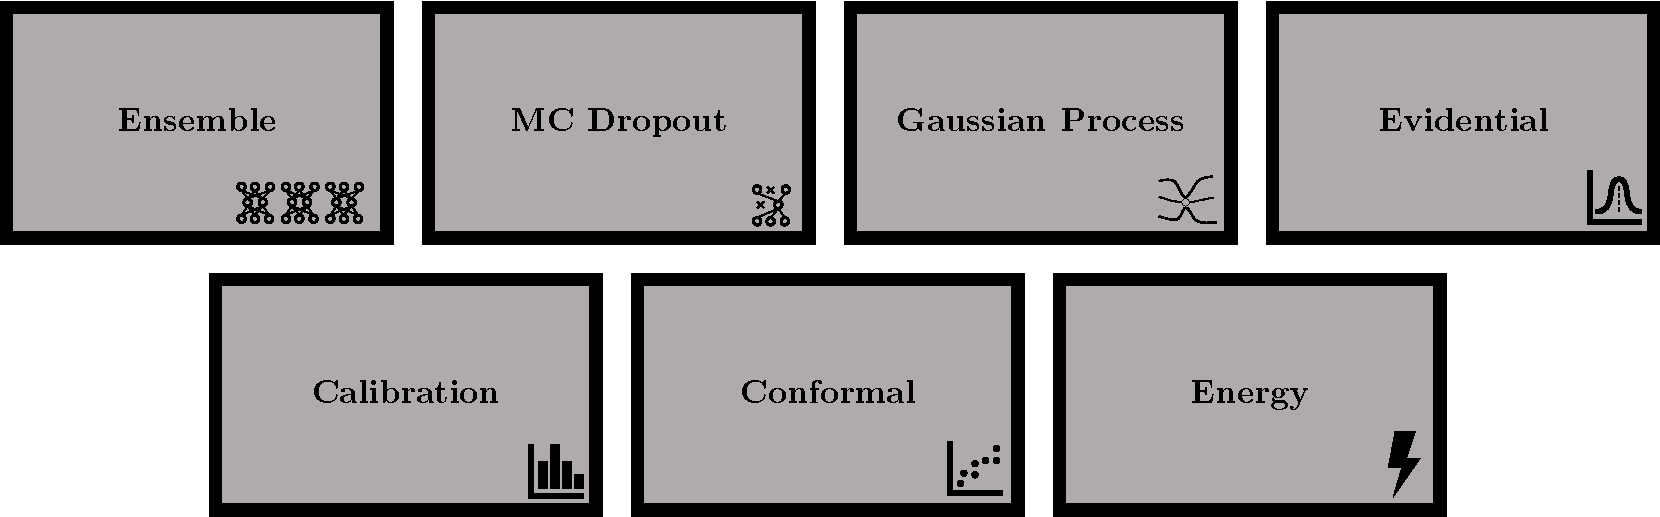
\includegraphics[width=0.9 \textwidth]{resources/overview_methods.pdf}}}$
    \end{subfigure}%
    \caption{Overview of the different families of methods for uncertainty estimation.}
    \label{fig:overview_methods}
	% \vspace{-.5cm}
\end{figure}

% Add a table with useful existing implementations/packages of those methods

\paragraph*{Ensembles.} This family of methods consists in combining the predictions of a set of multiple models $f_{\bm{\phi}_1},\cdot, f_{\bm{\phi}_K}$ by using stacking, bagging, boosting, Bayesian averaging or other Bayesian combinations \citep{bayesian-averaging-to-combination}. The variance of the different model predictions can be viewed as uncertainty estimates. These uncertainty estimates can be considered Bayesian where the member weights are sampled from the posterior weight distribution, i.e. $\bm{\phi}_k \sim \prior(\bm{\phi} \condition \data)$. The ensembles can be \emph{homogeneous ensembles}, i.e. the models share the same architecture, be \emph{heterogeneous ensembles}, i.e. the models have different architectures, or \emph{implicit ensembles}, i.e. a single model approximated ensembles parameter sampling \citep{abe2022deep}. Further, the different models can be trained sequentially (see e.g. \citep{schapire2013explaining, chenG16xgboost}) or independently (see e.g. \citep{ensembles}).
%
Ensembles are considered as strong baselines in terms of uncertainty estimation and predictive performances \citep{dataset-shift}. Ensembles also benefit from a simple implementation \citep{ensembles}.
%
Ensembles are often considered to be expensive as they require multiple forward passes. Many approaches \citep{batch-ensembles,mimo-independent-subnetworks} proposed to make faster ensembles. Further, while ensembles improve predictive performance, this performance gain can actually be replicated through the use of (larger) single models \citep{abe2022deep}.

\paragraph*{Variational Inference.} This family of methods consists in approximating a (generally intractable) posterior distribution with a variational distribution belonging to a tractable family of distributions \cite{blei2017vi}. The approximate posterior distribution is often optimized using an Evidence Lower Bound (ELBO) loss. Many methods (see e.g. \cite{practical-bnn,bayesian-networks,practical_deep_bayesian_principles}) are interested in the posterior distribution over the model weights, i.e. $\prior(\bm{\phi} \condition \data)$ where $\bm{\phi}$ are the model weights. Thus, similarly to ensembles, uncertainty estimates can be obtained by sampling from the posterior distribution on the weights and computing the variance of their predictions. These methods generally needs to trade off the expressivity of the posterior distribution with computational complexity. To approximate the posterior distribution over the high dimensional weights, many works proposed to use techniques like mean-field approximations \citep{practical-bnn,bayesian-networks,practical_deep_bayesian_principles}, normalizing flows \cite{radialflow,Louizos2017}, or matrix decomposition with low rank or Kronecker products \cite{mishkin2018slang,bae2018eigen,zhang2017noisy}. In contrast with methods which are interested in posterior distributions $\prior(\bm{\phi} \condition \data)$ over model weights $\bm{\phi}$, we present in this thesis variational methods which approximate the posterior distribution $\prior(\bm{\theta} \condition \data, \x)$ over the target distribution parameters $\bm{\theta}$ (see \cref{chap:classification,chap:regression}).

\paragraph*{Monte Carlo Dropout.} Monte Carlo (MC) dropout consists in randomly dropping neurons to form different models $f_{\bm{\phi}_1},\cdot, f_{\bm{\phi}_K}$ and combine their predictions \citep{dropout} at both training and testing time. This approach can be considered as an ensemble of implicit models \citep{abe2022deep} but also as performing variational inference \citep{dropout}. Hence, similarly to ensembles, the variance of the predictions can be viewed as Bayesian uncertainty estimates the member weights are sampled from the posterior weight distribution, i.e. $\bm{\phi}_k \sim \prior(\bm{\phi} \condition \data)$. Many works extended this approach for e.g. convolutional layers \citep{tassi2020bayesian} or dropping connection instead of activations \citep{wan2013dropconnect}.

\paragraph*{Markov Chain Monte Carlo.} Markov Chain Monte Carlo (MCMC) methods, consists in building a Markov Chain which will converge to samples from the posterior distribution. A key example is the Metropolis-Hastings algorithm which iteratively draw a sample from a transition rule and then decide to accept or reject it \cite{robert2015metropolis}. Many works focus on sampling from the approximate posterior distribution $\prior(\bm{\phi} \condition \data)$ over model weights $\bm{\phi}$ (see e.g. \citep{duane1987hybrid,welling2011langevin}). In this case, the Markov Chain builds a sequence $\bm{\phi},\cdot,\bm{\phi}_t$ by following e.g. Hamiltonian dynamics \citep{duane1987hybrid} or Stochastic Gradient Langevin Dynamics \cite{welling2011langevin,garriga-alonso2021exact,ma2015mcmc} which converge to sample from the posterior distribution, i.e. $\bm{\phi}_t \sim \prior(\bm{\phi} \condition \data)$ when $t \rightarrow \infty$. On one hand, while full batch MCMC has managed to scale to modern tasks and models, they often come at a heavy computational cost \citep{what-bnn-posterior}. On the other hand, while stochastic gradient MCMC improve the computational efficiency \cite{welling2011langevin,garriga-alonso2021exact,ma2015mcmc}, it might introduce bias in the stationary distribution by omitting the Metropolis-Hasting rejection or subsampling the data \citep{betancourt2015data,what-bnn-posterior}.

\paragraph*{Laplace Approximation.} The Laplace approximation consists in approximating the posterior distribution with a Gaussian distribution centered around a mode of the posterior distribution. Many works focus on approximating the posterior distribution $\prior(\bm{\phi} \condition \data)$ over model weights $\bm{\phi}$. In this case the Laplace approximation gives:
\begin{align*}
    \prior(\bm{\phi} \condition \data) \approx \DNormal(\bm{\phi}_\text{MAP}, \bm{\Sigma})
\end{align*}
where $\bm{\phi}_\text{MAP}$ is the maximum a posteriori estimate, and $\bm{\Sigma}=-(\nabla_{\bm{\phi}}^2 \left.\loss(\data;\bm{\phi})\right|_{\bm{\phi}_\text{MAP}})^{-1}$ is the Laplace approximation of the covariance based on the Hessian of the loss. The posterior distribution can be defined on all model weights, subnetworks \cite{daxberger2021bayesian}, or only the last layer \cite{bayesian-a-bit}. The Hessian computation can be costly and can be approximated using the different techniques like the Fisher information matrix, the generalized Gauss-Newton matrix, diagonal factorization, Kronecker-factored approximate curvature, or low-rank approximation \citep{daxberger2021laplace}. Finally, the computation of the predictive distribution needs further approximation like linearizing the neural network or using Monte-Carlo approximation \citep{daxberger2021laplace}.

\paragraph*{Gaussian Process.} Gaussian Processes (GPs) are a family of Bayesian methods which, given a dataset $\data$, associates to each new input $\x$ a predictive Gaussian distribution over the output $\y \sim \prob(\y \condition \data, \x) = \DNormal(m(\x), \sigma^2(\x))$. The mean function $m(\x)$ and the variance function $\sigma^2(\x)$ depends on the kernel function $\kappa(.,.)$ which encodes the similarity between data samples. Intuitively, uncertainty estimates can be obtained by computing the variance or the entropy of the predicted Gaussian distribution.
On one hand, standard GPs have computational and storage limitations \cite{jakkala2021deepgp}. E.g. the computation of the variance function is cubic in the number of data samples which does not scale well to large datasets. To mitigate this issue, previous works proposed sparse Gaussian process which introduce variational pseudo-points can be optimized with stochastic gradient descent (see e.g. \cite{snelson2005sparse,titsias2010gplvm,due}).
On the other hand, standard GPs does not naturally extract hierarchical representations from structured data. To mitigate this issue, previous works proposed e.g. to use multilayer GPs \cite{damianou2012deepgp} or deep neural networks as the kernel function \cite{wilson2016stochastic}. We refer to existing survey on Gaussian process in deep learning for further details \citep{gp-for-ml,damianou2012deepgp,jakkala2021deepgp}.

\paragraph*{Evidential.} Evidential methods are derived from the theory of evidence which can be seen as generalization of the Bayesian theory to subjective probables \cite{dempster1968evidence,shafer1976mathematical}. Instead of predicting directly the parameters $\bm{\theta}$ of the target distribution $\prob(\y \condition \bm{\theta})$, evidential methods consist in predicting the parameters of the distribution $\prior(\bm{\theta} \condition \data, \x)$ defined over the parameters $\bm{\theta}$, thus following the factorization in \cref{eq:factorization_3}. In this case, uncertainty estimates can be obtained by computing the variance or the entropy of the predicted target or evidential distributions. This family of models is generally effective since it only requires a single forward pass for uncertainty estimation. To improve performances of evidential models, other works proposed to use OOD data during training \cite{PriorNetworks,reverse-kl}, knowledge distillation \cite{distribution-distillation}, or contrastive learning \cite{uncertainty-generative-classifier}. In this thesis, we introduce a new family of evidential models called \emph{Posterior networks} with a clear Bayesian interpretation and low practical overhead (see \cref{chap:classification,chap:regression,chap:robustness,chap:graph_data,chap:sequential_data,chap:reinforcement_learning}). We refer to existing survey on evidential deep learning for uncertainty quantification for further details \citep{survey_evidential_uncertainty}.

\paragraph*{Calibration.} Calibration metrics consists at evaluating if the probabilities predicted by a model correspond to the true probabilities of the model to be correct (see \cref{sec:calibration} for further details). Hence, in order to achieve high performance w.r.t. calibration metrics, calibration methods aim at predicting probabilities which are good approximations of their true probability of correctness. Beyond uncertainty-aware models which are expected to be well-calibrated, we distinguish between two other groups of calibration methods: during-training calibration methods and post-training calibration methods. During-training calibration methods apply regularization techniques in the loss objective to create inherently calibrated models (see e.g. \cite{lee2018training,corbieres2019confidence,minderer2021revisiting}). Post-training calibration methods recalibrate the model predictions after training (see e.g. \cite{calibration-network,wenger201calibration}). While these methods can adapt well to different architectures types, they usually require additional held-out validation data and assume that validation and test distribution are similar. Prominent classes of post-training calibration method are histogram binning \cite{zadrozny2001calibrated}, Temperature scaling \cite{calibration-network}, isotonic calibration \cite{zadrozny2002transforming}, Dirichlet calibration \cite{kull2019beyond}, or conformal predictions \cite{conformal-survey,marx2022conformal}.

\paragraph*{Density-based models.} This family of models assigned to every data sample $\x$ a probability density estimate $\prob(\x \condition \bm{\phi})$. In this case, a data sample considered uncertain by the model should be assigned a low density value while a data sample considered certain for the model should be assigned a high density value. The density estimator can be of different nature like a mixture of Gaussian \cite{simple_ood_adv_detection,du2022vos} or a normalizing flow \cite{nf-review,why-nf-fail-ood,postels2020hiddenuncertainty}. The choice of space on which the density estimator operates is crucial. While density estimation on the input space might be difficult due to the curse of dimensionality \citep{anomaly-detection,deep-generative,typicality_OOD_generative}, other works \cite{charpentier2020, why-nf-fail-ood, density-states-ood, contrastive-ood} improved the performance of density-based methods on uncertainty tasks by leveraging a task-induced bias or low-dimensional statistics. In particular, density-based models methods have achieved impressive success in OOD detection tasks \cite{ood-detection-survey}.

\paragraph*{Energy-based models.} Energy-based models (EBMs) associate to every combination of input $\x$ and output $\y$, a scalar energy value $E_{\bm{\phi}}(\y, \x)$ \cite{lecun2006tutorial}. Interestingly, EBMs can often be viewed as density-based models. Indeed, the energy function $E_{\bm{\phi}}(\y, \x)$ can be transformed into Gibbs distributions $\prob(\y \condition \bm{\phi}, \x)$, $\prob(\y, \x \condition \bm{\phi})$, or even $\prob(\x \condition \bm{\phi})$ given some integrations constraints on $E_{\bm{\phi}}(\y, \x)$, thus assigning uncertainty estimates on for different combinations of variables $\y, \x$ \cite{energy_based_classifier}. In this case, low predicted energy values correspond to high uncertainty estimates. EBMs are flexible models capable to achieve great performances in OOD detection in many tasks \citep{energy-ood,wang2021ebm} as long as they can capture semantic features of the data \cite{ood_ebm}.

\paragraph*{Distance-based models.} The core idea of distance-based methods is that the model should assign high uncertainty to testing data samples which are far away from training data samples. Hence, distance-based models can e.g. use distance to class centroids \cite{mohseni2020self}, nearest-neighbor \cite{sun2022knnood}, or inducing points \cite{due} to estimate uncertainty. Further, they can also use Mahalanobis distance \cite{mohseni2020self}, euclidean distance \cite{huang2021feature}, or geodesic distance \cite{gomes2022igeood}. Similarly to density-based models, distance-based models can also achieve great performance in OOD detection tasks \cite{ood-detection-survey}. Further, distance awareness has been shown to be an important component for uncertainty estimation tasks \cite{uncertainty-distance-awareness,due}.

% \subsection{Sampling-based models}
% Sampling-based models estimate uncertainty by aggregating statistics (e.g. mean and variance) from different samples from a given distribution. The prediction generally follows a three steps process:
% \textbf{(1)} we sample $K$ model weights $\bm{\phi}_k$ from a distribution over the weights $\prior(\bm{\phi} \condition \data)$, i.e. $\bm{\phi}_k \sim \prior(\bm{\phi} \condition \data)$. The type of the weight distribution $\prior(\bm{\phi} \condition \data)$ is a key design choice. E.g. ensemble proposes to train independent model weights \cite{ensembles}, MC dropout randomly drop weights with given dropout rate \cite{dropout}, and other Bayesian neural networks learn explicit distributions like Gaussian over the model weights \cite{bayesian-networks}. \textbf{(2)} We perform $K$ forward passes with the sampled model weights to obtain parameters $\bm{\theta}_k$ of the target distribution, i.e. $\bm{\theta}_k = f_{\bm{\phi}_k}(\x) \text{ for } k=\{1,\cdot,K\}$. This allows to implicitly sample the parameters $\bm{\theta}_k$ from the posterior distribution $\prior(\bm{\theta} \condition \data, \x)$, i.e. $\bm{\theta}_k \sim \prior(\bm{\theta} \condition \data, \x)$. In this case, the parameters $\bm{\theta}_k$ can be the parameters of a categorical distribution for classification or the parameters of a Gaussian distribution for regression. \textbf{(3)} We aggregate the $\bm{\theta}_k$ parameters to form a point estimate $\bm{\theta}*$, e.g. $\bm{\theta}*=\frac{1}{K}\sum_k \bm{\theta}_k$. This allows to define the target distribution $\prob(\y \condition \bm{\theta}^*)$. These methods are flexible and allows to estimate all types of uncertainty while still being accurate. However, they often come to the cost of a higher computational cost due to the need of multiple forward passes.

% \subsection{Sampling-free models}
% Sampling-free models are capable of estimating uncertainty in a single forward pass. A first family of models explicitly parametrize the distribution $\prior(\bm{\theta} \condition \data, \x)$ with evidential distributions \citep{survey_evidential_uncertainty,robustness-uncertainty-dirichlet,max_gap_id_ood,uncertainty-generative-classifier,multifaceted_uncertainty,graph-postnet, lightweight-prob-net}. A second family aims at learning deep Gaussian processes on a learned latent space \citep{uncertainty-distance-awareness, due, duq, uceloss}. A third family aims at learning deep energy-based models \citep{ood_ebm, jem_ebm}. The GP and energy-based approaches might sometimes not be able to disentangle the different uncertainty types. Another family of models tries to recalibrate existing models by using calibration methods like temperature scaling \cite{calibration-network} or conformal predictions \cite{conformal-survey}. Calibration and conformal prediction methods generally require additional data to calibrate uncertainty estimates. Finally, a last family of models propagate uncertainty across layers \citep{natural-parameter-network, sampling-free-variance-propagation, feed-forward-propagation, lightweight-prob-net, probabilistic-backprop-scalable-bnn}. They model uncertainty at the weight and/or activation levels and are generally constrained to specific transformations.

\section{Uncertainty metrics}
\label{sec:background-experiments}

While ML models are primarily expected to provide accurate predictions, we present in this section an exhaustive summary of the main metrics used to evaluate the quality of uncertainty estimation. 
It covers correct/wrong predictions detection, OOD \& dataset shifts detection, calibration, and sample efficiency.
We provide a collection of evaluation setups covering various tasks to benchmark uncertainty models in \cref{tab:overview_evaluation}. Beyond these metrics, note that Bayesian methods have been also used in other tasks like  model pruning, model selection, or hyper-parameter tuning \citep{bayesian-networks,daxberger2021laplace}.

\begin{table*}[ht]
    \begin{center}
    \resizebox{1.\textwidth}{!}{%
    \begin{tabular}{ccc}
    \toprule
    \textbf{Uncertainty metrics} & \textbf{Existing evaluation setups} & \textbf{Practical reason}\\
    \midrule
    \midrule
    Uncertainty calibration & \cite{dataset-shift, chung2021uncertainty,nado2021uncertainty, tran2022plex} & \emph{Fairness}, \emph{Trust}\\
    \midrule
    Correct/wrong pred. detection & \cite{robustness-uncertainty-dirichlet,Hendrycks2016, shifts-dataset, tran2022plex} & \emph{Trust} \\
    \midrule
    OOD detection & \cite{robustness-uncertainty-dirichlet,charpentier2022uncertainty-rl,yang2022openood, cao2020ood, kirchheim2022pytorch, Hendrycks2016,charpentier2022uncertainty-rl, tran2022plex} & \emph{Safety}\\
    \midrule
    Robustness to dataset shifts & \cite{robustness-uncertainty-dirichlet,wilds, neuhold201mapillary, shifts-dataset, benchmarking-corruptions, taori2020shift, dataset-shift, croce2021robustbench,charpentier2022uncertainty-rl, tran2022plex} & \emph{Maintenance} \\
    \midrule
    Sample efficiency & \cite{charpentier2022uncertainty-rl,hsu2018continual, lin2021clear,antoniou2020fewshots,tran2022plex} & \emph{Development, Maintenance}\\
    \bottomrule
    \end{tabular}%
    }
    \end{center}
    \caption{Overview of metrics for uncertainty estimation. We relate each of the uncertainty metric to existing evaluation setups and practical reason for uncertainty estimation presented in \cref{sec:why_uncertainty}}
    \label{tab:overview_evaluation}
\end{table*}

\subsection{Uncertainty Calibration}
\label{sec:calibration}

It is crucial to provide confidence intervals accurately reflecting the true chance of an event to happen. This allows to increase \emph{fairness} and \emph{trust} of the ML prediction even on under-represented data regions. Intuitively, if the model predict $80\%$ chance for a class to be the correct one, we would expect the model to be $80\%$ of the time correct. Hence, uncertainty estimates are important to answer the following practical question:

\begin{center}
    \textbf{Do probabilities predicted by ML models correspond to the true probabilities?}
\end{center}

In practice, the confidence intervals provided by the models can be used to estimate risks when making decisions. Appropriate metrics to evaluate calibration involve (strictly) proper scoring rules like Brier scores for classification and quantiles scores for regression \cite{scoring-rules}.

\subsection{Correct \& Wrong Predictions}

It is also crucial to detect when ML models are likely to provide correct or wrong predictions. This allows to increase \emph{trust} in the model predictions, especially when the predictions are used to make important decisions. Intuitively, while the model predictions should be accurate, uncertainty estimates should also be good indicators of the prediction errors. Indeed, high uncertainty should indicate likely wrong prediction while low uncertainty should indicate likely correct predictions. Hence, uncertainty estimates are important to answer the following practical question:

\begin{center}
    \textbf{Can we detect prediction errors of ML models?}
\end{center}

In practice, each application would require to set a threshold on the uncertainty estimates. Ideally, while predictions associated with uncertainty estimates below this threshold should be correct, the predictions associated with uncertainty estimates above this threshold should be wrong. Hence, we can use evaluation metrics which compare scores (i.e. uncertainty estimates) with binary classes (i.e. correct/wrong predictions). Common metrics are based on false and true positive and negative rates given a specific threshold like precision, recall, or F1 score \cite{powers2011evaluation}. However, these metrics have the important limitation to depend on a specific choice of threshold. Instead, there exist other evaluations like receiving operator curves (ROC) and precision-recall curves (PR) which can compare the prediction correctness and the predicted uncertainty scores for any choice of threshold. In particular, the area under the ROC curve (AUC-ROC) and the area under the PR curve (AUC-PR) are appropriate metrics to evaluate the overall performance of the uncertainty scores independently of the choice of threshold \cite{apr_auroc}. All the data used for the evaluation of the correct/wrong predictions should be relevant to the task meaning that every input has a corresponding output label. This requirement contrasts data used for out-of-distribution detection data where inputs might not have corresponding labels.

\subsection{Out-Of-Distribution}

It is crucial to detect when incoming data are anomalous to increase the \emph{safety} of model predictions. The anomalous data are often considered out-of-distribution (OOD) in contrast with normal data similar to data observed during training which are considered in-distribution (ID). Intuitively, uncertainty estimates should be good indicators of anomalous data. Indeed, high uncertainty should indicate likely abnormal data while low uncertainty should indicate likely normal data. Hence, uncertainty estimates are important to answer the following practical question:

\begin{center}
    \textbf{Can uncertainty estimates detect anomalous data?}
\end{center}

Similarly to the detection of correct and wrong predictions, the detection of anomalous data would also require to set a threshold on the uncertainty estimates. In this case, while predictions associated with uncertainty estimates below this threshold should be normal ID data, predictions associated with uncertainty estimates above this threshold should ideally be abnormal OOD data. Hence, we can also use evaluation metrics like precision, recall, AUC-ROC, and AUC-PR which compare scores (i.e. uncertainty estimates) with binary classes (i.e. ID/OOD data). While ID data should be relevant to the task (i.e. ID inputs have output labels), the OOD data should be clear anomalies (e.g. OOD data come from a different dataset) and might not be relevant to the task (e.g. OOD data are noisy inputs without output labels).

\subsection{Dataset Shifts}

It is crucial to detect and be robust against shifts in the data to primarily increase the ease of \emph{maintenance} of ML models. Intuitively, while the predictions should be robust to dataset shifts, the uncertainty estimates should increase under dataset shifts. Hence, uncertainty estimates are able to indicate when the incoming data drifts away from the training data before that the model breaks. Hence, uncertainty estimates are important to answer the following practical question:

\begin{center}
    \textbf{Are model predictions robust to data shift?}
\end{center}

In practice, the model would require to \emph{jointly} look at the evolution of the accuracy and the uncertainty estimates under different magnitudes of perturbations. Ideally, while the model should maintain high accuracy on shifted data (a.k.a. OOD generalization performance \cite{ood-generalization-survey}), the uncertainty estimates of the model should increase on shifted data (a.k.a. OOD detection performance \cite{ood-detection-survey}). Further, other expectations on the predictions under dataset shifts involve maintaining good calibration \cite{dataset-shift}, high correct/wrong prediction detection performance (see \cref{chap:robustness}), and high OOD detection performances (see \cref{chap:robustness}). In this case, the shifted dataset is still relevant to the original task (i.e. inputs in the shifted dataset have output labels) but differ from the original ID dataset. We distinguish between natural and adversarial dataset shifts. Natural shifts correspond to natural perturbations which could occur in real world scenarios like time shifts \cite{wilds, neuhold201mapillary, shifts-dataset}, location shifts \cite{wilds, neuhold201mapillary, shifts-dataset}, or corrupted data \cite{benchmarking-corruptions, taori2020shift}. In contrast, adversarial perturbations shifts actions correspond to the worst-case scenario where the perturbations are designed to fool the model.

\subsection{Sample efficiency}

It is crucial to wisely select data samples to learn efficiently while avoiding failures. This allows to ease the \emph{development} and \emph{maintenance} of the ML models by reducing training time, number of model failures, or enabling to continually learn from the environment. Intuitively, samples with high confidence might not be interesting since already learned, while samples with too high uncertainty might not be irrelevant outliers Hence, uncertainty estimates are important to answer the following practical question:

\begin{center}
    \textbf{How can uncertainty estimates efficiently select data samples to learn from?}
\end{center}

In practice, the sample selection process is particularly relevant in reinforcement learning (see \cref{chap:reinforcement_learning}), active learning (e.g. \cite{gal2017bald, kirsch2019batch}), continual learning \cite{hsu2018continual, lin2021clear}, or few-shots learning \cite{antoniou2020fewshots}. Appropriate metrics would be e.g. to measure the training speed by counting the required number of training samples or the time to train.


\part{Uncertainty Estimation for I.I.D. data}
\chapter{Uncertainty Estimation for Classification}
\label{chap:classification}

\section{Introduction}
\label{sec:introduction_006}

Quantifying uncertainty in neural network predictions is key to making Machine Learning reliable. In many sensitive domains, like robotics, financial or medical areas, giving autonomy to AI systems is highly dependent on the trust we can assign to them. In addition, AI systems being aware about their predictions' uncertainty, can adapt to new situations and refrain from taking decisions in unknown or unsafe conditions. Despite of this necessity, traditional neural networks show overconfident predictions, even for data that is signifanctly different from the training data \cite{ensembles} \cite{calibration-network}. 
In particular, they should distinguish between \emph{aleatoric} and \emph{epistemic} uncertainty, also called data and knowledge uncertainty \cite{PriorNetworks}, respectively. The aleatoric uncertainty is irreducible from the data, e.g. a fair coin has 50/50 chance for head. The epistemic uncertainty is due to the lack of knowledge about unseen data, e.g. an image of an unknown object or an outlier in the data.

\begin{figure}[ht!]
    \centering
    \begin{subfigure}[t]{0.23 \columnwidth}
        \centering
        
\includegraphics[width=0.8 \textwidth]{sections/006_neurips2020/figures/2D_latent_klpn_2.png}
         \caption{Data labels - PriorNet}
         \label{KLPN_visualization_2D}
    \end{subfigure}%
    \begin{subfigure}[t]{0.23\columnwidth}
        \centering
        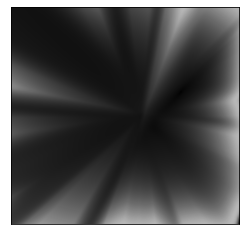
\includegraphics[width=0.8 \textwidth]{sections/006_neurips2020/figures/2D_latent_klpn_1.png}
        \caption{Uncertainty - PriorNet}
        \label{KLPN_visualization_unc}
    \end{subfigure}%
    \begin{subfigure}[t]{0.23 \columnwidth}
        \centering
        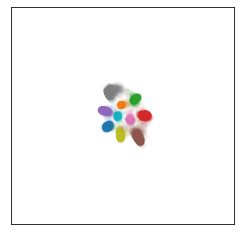
\includegraphics[width=0.8 \textwidth]{sections/006_neurips2020/figures/2D_latent_ours_bn_2.png}
         \caption{Data labels - \PostNetacro}
         \label{ours_visualization_2D}
    \end{subfigure}%
    \begin{subfigure}[t]{0.23\columnwidth}
        \centering
        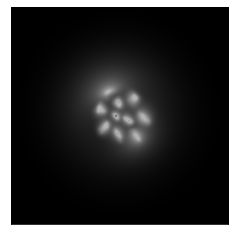
\includegraphics[width=0.8 \textwidth]{sections/006_neurips2020/figures/2D_latent_ours_bn_1.png}
        \caption{Uncertainty - \PostNetacro}
        \label{ours_visualization_unc}
    \end{subfigure}%
    \caption{PriorNet has a pre-ultimate layer of dimension $2$ and was trained with Reverse KL and uniform noise on $[0,255]^{28\times28}$ as OOD data. \PostNetacro has a latent space of dimension $2$ and was trained without OOD data. (a) and (c) show the learned latent positions of data with colored labels. (b) and (d) show uncertainty estimates in the latent spaces where darker regions indicate high uncertainty. \PostNetacro correctly assigns high uncertainty to OOD regions contrary to PriorNet.}
    \label{fig:mnist_2D_latent_space}
	% \vspace{-.5cm}
\end{figure}

\paragraph{Related work.} Uncertainty estimation is a growing research area unifying various approaches \cite{bayesian-networks, simple-baseline-uncertainty, practical_deep_bayesian_principles, Eswaran2017, ensembles, dropout}. Bayesian Neural Networks learn a \emph{distribution} over the weights \cite{bayesian-networks, simple-baseline-uncertainty, practical_deep_bayesian_principles}. Another class of approaches uses a collection of sub-models and aggregates their predictions, which are in turn used to estimate statistics (e.g., mean and variance) of the class probability distribution. Even though such methods, like ensemble and drop-out, have demonstrated remarkable performance (see, e.g., \cite{dataset-shift}), they describe implicit distributions for predictions and require a costly sampling phase at inference time for uncertainty estimation. 

Recently, a new class of models aims to directly predict the parameters of a prior distribution on the categorical probability predictions, accounting for the different types of uncertainty \cite{PriorNetworks, reverse-kl, sensoy2018, uceloss}. However, these methods require (i) the definition of arbitrary target prior distributions \cite{PriorNetworks, reverse-kl, sensoy2018}, and most importantly, (ii) out-of-distribution (OOD) samples during training time, which is an unrealistic assumption in most applications \cite{PriorNetworks, reverse-kl}.

Classically, these models would use both ID and OOD samples (e.g. MNIST and FashionMNIST) during training to detect similar OOD samples (i.e. FashionMNIST) at inference time. We show that preventing access to explicit OOD data during training leads to poor results using these approaches (see Fig.~\ref{fig:mnist_2D_latent_space} for MNIST; or app. for toy datasets). Contrary to the expected results, these models produce increasingly confident predictions for samples far from observed data. In contrast, we propose \PostNet (\PostNetacro), which assigns high epistemic uncertainty to out-of-distribution samples, low overall uncertainty to regions nearby observed data of a single class, and high aleatoric and low epistemic uncertainty to regions nearby observed data of different classes.

\PostNetacro uses normalizing flows to learn a distribution over Dirichlet parameters in latent space. We enforce the densities of the individual classes to integrate to the number of training samples in that class, which matches well with the intuition of Dirichlet parameters corresponding to the number of observations per class. \PostNetacro does not require any OOD samples for training, the (arbitrary) specification of target prior distributions, or costly sampling for uncertainty estimation at test time.

\section{\PostNet}
\label{sec:model_006}

In classification, we can distinguish between two types of uncertainty for a given input $\vect{x}\dataix$: the uncertainty on the class prediction \smash{$y\dataix \in \{1, \ldots, \nclass\}$} (i.e.\ aleatoric unceratinty), and the uncertainty on the categorical distribution prediction \smash{$\vect{p}\dataix = [p\dataix_1, \ldots, p\dataix_\nclass]$} (i.e.\ epistemic uncertainty). A convenient way to model both is to describe the \emph{epistemic distribution} \smash{$q\dataix$} of the categorical distribution prediction \smash{$\vect{p}\dataix$}, i.e.\ \smash{$\vect{p}\dataix \sim q\dataix$}. From the epistemic distribution follows naturally an estimate of the \emph{aleatoric distribution} of the class prediction \smash{$y\dataix \sim \text{Cat}(\bar{\vect{p}}\dataix)$} where \smash{$\E_{q\dataix}[\vect{p}\dataix] = \bar{\vect{p}}\dataix$}.

Approaches like ensembles \cite{ensemble_simple} and dropout \cite{drop_out} model $q\dataix$ implicitly, which only allows them to estimate statistics at the cost of $S$ samples (e.g. \smash{$\E_{q\dataix}[\vect{p}\dataix] \approx \frac{1}{S}\sum_{s=1}^{S} \tilde{\vect{p}}\dataix$} where \smash{$\tilde{\vect{p}}\dataix$} is sampled from \smash{$q\dataix$}). 
%
Another class of models \cite{prior_net, rev_kl_prior_net, uceloss, evidential_uncertainty} explicitly parametrizes the epistemic distribution with a Dirichlet distribution (i.e.\ \smash{$q^{(\idata)} = \text{Dir}(\bm{\alpha}\dataix)$} where \smash{$f_{\theta}(x\dataix) = \bm{\alpha} \dataix \in \mathbb{R}_+^\nclass$}), which is the natural prior for categorical distributions. This parametrization is convenient since it requires only one pass to compute epistemic distribution, aleatoric distribution and class prediction:
\begin{equation}
\begin{aligned}
q^{(\idata)} &= \text{Dir}(\bm{\alpha}\dataix),\hspace{25pt} 
\bar{p}_\iclass\dataix &= \frac{\alpha_\iclass}{\alpha_0} \text{ with } \alpha_0 = \sum^{\nclass}_{\iclass=1} \alpha_\iclass,\hspace{25pt}
y^{(\idata)} &= \arg \max \;[\bar{p}_1, ..., \bar{p}_\nclass]
\end{aligned}
\end{equation}
The concentration parameters \smash{$\alpha\dataix_\iclass$} can be interpreted as the number of observed samples of class $\iclass$ and, thus, are a good indicator of epistemic uncertainty for non-degenerate Dirichlet distributions (i.e.\ \smash{$\alpha\dataix_\iclass \geq 1$}). To learn these parameters, Prior Networks \cite{prior_net, rev_kl_prior_net} use OOD samples for training and define different target values for ID and OOD data. For ID data, \smash{$\alpha\dataix_\iclass$} is set to an arbitrary, large number if $\iclass$ is the correct class and $1$ otherwise. For OOD data, \smash{$\alpha\dataix_\iclass$} is set to $1$ for all classes. 

This approach has four issues:
%\begin{itemize}
    %\item 
    \textbf{(1)} The knowledge of OOD data for training is unrealistic. In practice, we might not have these data, since OOD samples are by definition not likely to be observed.
    %\item 
    \textbf{(2)} Discriminating in- from out-of-distribution data by providing an explicit set of OOD samples is hopeless. Since any data not from the data distribution is OOD, it is therefore impossible to characterize the infinitely large OOD distribution with an explicit data set.
    %\item 
    \textbf{(3)} The predicted Dirichlet parameters can take any value, especially for new OOD samples which were not seen during training. In the same way, the sum of the total fictitious prior observations over the full input domain $\int \alpha_0(\vect{x}) d\vect{x}$  is not bounded and in particular can be much larger than the number of ground-truth observations $N$. This can result in undesired behavior and assign arbitrarily high epistemic certainty for OOD data not seen during training.
    %\item 
    \textbf{(4)} Besides producing such arbitrarily high prior confidence, PNs can also produce degenerate concentration parameters (i.e.\ $\alpha_\iclass$ < 1). While \cite{rev_kl_prior_net} tried to fix this issue by using a different loss, nothing intrinsically prevents Prior Networks from predicting degenerate prior distributions.
%\end{itemize}
In the following section we describe how \PostNet solves these drawbacks.

\subsection{An input-dependent Bayesian posterior}

First, recall the Bayesian update of a single categorical distribution \smash{$y \sim \text{Cat}(\vect{p})$}. It consists in (1) introducing a prior Dirichlet distribution over its parameters i.e. \smash{$\prob(\vect{p}) = \text{Dir}(\bm{\beta^\text{prior}})$} where \smash{$\bm{\beta^\text{prior}} \in \mathbb{R}_+^\nclass$}, and (2) using $N$ given observations \smash{$y^{(1)},..., y^{(N)}$} to form the posterior distribution $\prob(\vect{p}|\{y^{(j)}\}_{j =1}^N)= \text{Dir}(\bm{\beta^\text{prior}} + \bm{\beta^\text{data}})$ where \smash{$\beta^\text{data}_\iclass = \sum_j \mathbb{1}_{y^{(j)}=\iclass}$} are the class counts. That is, the Bayesian update is
\begin{equation}
    \begin{aligned}
    \prob(\vect{p}|\{y^{(j)}\}_{j =1}^n) \propto \prob(\{y^{(j)}\}_{j =1}^n|\vect{p}) \times \prob(\vect{p}).
    \end{aligned}
\end{equation}
Observing no data (i.e. $\beta_\iclass^\text{data} \rightarrow 0$) would lead to flat categorical distribution (i.e. \smash{$p_\iclass = {\beta_\iclass^{\text{prior}}}\cdot ({\sum_{\iclass'}\beta_{\iclass'}^{\text{prior}}})^{-1}$}), while observing many samples (i.e. \smash{$\beta_\iclass^\text{data}$} is large) would converge to the true data distribution (i.e. $p_\iclass \approx \frac{\beta_\iclass}{\sum_i\beta_i}$).
Furthermore, we remark that $N$ behaves like a certainty budget distributed over all classes i.e. \smash{$N = \sum_\iclass \beta^\text{data}_\iclass$}.

Classification is more complex. Generally, we predict the class label \smash{$y\dataix$} from a different categorical distribution \smash{$\text{Cat}(\vect{p}\dataix)$} for each input \smash{$\vect{x}\dataix$}. \PostNetacro extends the Bayesian treatment of a single categorical distribution to classification by predicting an individual posterior update for any possible input. To this end, it distinguishes between a fixed prior parameter \smash{$ \bm{\beta}^{\text{prior}}$} and the additional learned (pseudo) counts \smash{$\bm{\beta}\dataix$} to form the parameters of the posterior Dirichlet distribution \smash{$\bm{\alpha}\dataix = \bm{\beta}^{\text{prior}} + \bm{\beta}\dataix$}. 
%\bc{Remark that directly using the single label \smash{$y\dataix$} to learn independently the posterior for input \smash{$\vect{x}\dataix$ (i.e. $\beta_\iclass\dataix = 1$} for the true class and \smash{$\beta_\iclass\dataix = 0$} otherwise) would lead to a poor uncertainty estimate and more importantly not generalize to new inputs}. 
Hence, \PostNetacro's posterior update is equivalent to predicting a set of pseudo observations \smash{$\{\tilde{y}^{(j)}\}_j\dataix$} per input \smash{$\vect{x}\dataix$}, accordingly \smash{$\beta_\iclass\dataix = \sum_j  \mathbb{1}_{\tilde{y}^{(j)}=\iclass}$} and
\begin{equation}
    \begin{aligned}
    \prob(\vect{p}\dataix|\{\tilde{y}^{(j)}\}_j\dataix) \propto \prob(\{\tilde{y}^{(j)}\}_j\dataix|\vect{p}\dataix) \times \prob(\vect{p}\dataix).
    \end{aligned}
\end{equation}
In practice, we set \smash{$\bm{\beta}^{\text{prior}}=\vect{1}$} leading to a flat equiprobable prior when the model brings no additional evidence, i.e.\ when \smash{$\bm{\beta}\dataix = \vect{0}$}. 

The parametrization of $\beta_\iclass\dataix$ is crucial and based on two main components. The first component is an encoder neural network, $f_{\theta}$ that maps a data point $\vect{x}\dataix$ onto a low-dimensional latent vector $\latent\dataix=f_{\theta}(\vect{x}\dataix) \in \mathbb{R}^{\latentdim}$. The second component is to learn a \textit{normalized} probability density $\prob(\latent | \iclass; \phi)$ per class on this latent space; intuitively acting as class conditionals in the latent space. Given these and the number of ground-truth observations $N_\iclass$ in class  $\iclass$, we define:
\begin{equation}
\begin{aligned}
\label{eq:additional_observations}
	\beta_\iclass\dataix &= N_\iclass \cdot \prob(\latent\dataix | c; \phi) = N \cdot \prob(\latent\dataix | \iclass; \phi) \cdot \prob(\iclass),
\end{aligned}
\end{equation}
which corresponds to the number of (pseudo) observations of class $\iclass$ at $\latent \dataix$. Note that it is crucial that $\prob(\latent | \iclass; \phi)$ corresponds to a proper normalized density function since this will ensure the model's epistemic uncertainty to increase outside the known distribution. Indeed, the core idea of our approach is to parameterize these distributions by a flexible, yet tractable family: normalizing flows (e.g. radial flow \cite{vi_flow} or IAF \cite{iaf_flow}). Note that normalizing flows are theoretically capable of modeling any continuous distribution given an expressive and deep enough model \cite{neural_flow, iaf_flow}.

In practice, we observed that various architectures can be used for the encoder. Also, similarly to GAN training \cite{GAN_batch_norm}, we observed that adding a batch normalization after the encoder made the training more stable. It facilitates the match between the latent positions output by the encoder and non-zero density regions learned by the normalizing flows. Remark that we can theoretically use any density estimator on the latent space. We experimentally compared Mixtures of Gaussians (MoG), radial flow \cite{vi_flow} and IAF \cite{iaf_flow}. While all density types performed reasonably well (see Tab.~\ref{fig:unc_sensorless_drive} and app.), we observed a better performance of flow-based density estimation in general. We decided to use radial flow for its good trade-off between flexibility, stability, and compactness (only few parameters).

\textbf{Model discussion.} Equation \ref{eq:additional_observations} exhibits a set of interesting properties which ensure reasonable uncertainty estimates for ID and OOD samples. To highlight the properties of the Dirichlet distributions learned by \PostNetacro, we assume in this paragraph that we have a fixed encoder $f_\theta$ and normalizing flow model parameterized by $\phi$. Writing the mean of the Dirichlet distribution parametrized by \eqref{eq:additional_observations} and using Bayes' theorem gives:
\begin{equation}
\E_{\vect{p}\sim \Dir(\boldsymbol{\alpha}\dataix)}[p_\iclass] = \frac{\beta_\iclass^\text{prior} + N \cdot \prob(\iclass | \latent\dataix; \phi) \cdot \prob(\latent\dataix; \phi)}{\sum_\iclass\beta_\iclass^\text{prior} + N \cdot \prob(\latent\dataix; \phi)}
\end{equation}
For very likely in-distribution data (i.e. $\prob(\latent\dataix ; \phi) \rightarrow \infty$), the aleatoric distribution estimate \smash{$\bar{\vect{p}}\dataix = \E_{\vect{p}\sim \Dir(\boldsymbol{\alpha}\dataix)}[p_\iclass]$} converges to the true categorical distribution \smash{$\prob(\iclass|\latent \dataix; \phi)$}. Thus, predictions are more accurate and calibrated for likely samples. Conversely, for out-of-distribution samples (i.e. \smash{$\prob(\latent\dataix ; \phi) \rightarrow 0$}), the aleatoric distribution estimate \smash{$\bar{\vect{p}}\dataix = \E_{\vect{p}\sim \Dir(\boldsymbol{\alpha}\dataix)}[p_\iclass]$} converges to the flat prior distribution (e.g. \smash{$p_\iclass=\frac{1}{\nclass}$} if \smash{$\bm{\beta}^{prior}=\vect{1}$}). In the same way, we show in the appendix that the covariance of the epistemic distribution converges to $\vect{0}$ for very likely in-distribution data, meaning no epistemic uncertainty. Thus, uncertainty for in-distribution data is reduced to the (inherent) aleatoric uncertainty and zero epistemic uncertainty.
%
Similarly to the single categorical distribution case, increasing the training dataset size (i.e. $N \rightarrow \infty$) also leads to the mean prediction $\E_{\vect{p}\sim \Dir(\boldsymbol{\alpha})}[p_\iclass]$ converging to the class posterior \smash{$\prob(c | \latent\dataix; \phi)$}. On the contrary, no observed data (i.e $N=0$) again leads to the model reverting to a flat prior.

\PostNet also handles limited certainty budgets at different levels. At the sample level, the certainty budget \smash{$\alpha_0\dataix = \sum_\iclass \alpha_\iclass\dataix$} is distributed over classes. At the class level, the certainty budget \smash{$N_\iclass = \int N_\iclass \; \prob(\latent | c; \phi) \; d\latent = N_\iclass  \int \prob(\latent | c; \phi) \; d\latent$} is distributed over samples. At the dataset level, the certainty budget \smash{$N = \sum_\iclass \int N_\iclass \; \prob(\latent | c; \phi) \; d\latent$} is distributed over classes and samples. Regions of latent space with many training examples are assigned high density $\prob(\latent | c; \phi)$, forcing low density elsewhere to fulfill the integration constraint. Consequently, density estimation using normalizing flows enables \PostNetacro to learn out-of-distribution uncertainty by observing only in-distribution data.

\begin{wrapfigure}[16]{r}{0.505\textwidth}
    \vspace{-.3cm}
	\resizebox{.505 \columnwidth}{!}{
	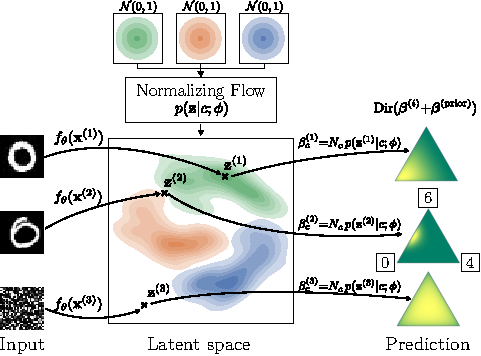
\includegraphics{sections/006_neurips2020/diagram/diagram_new-crop.pdf}
	}
	\caption{Overview of \PostNet.}
	\label{fig:overview}
	\vspace{-.5cm}
\end{wrapfigure}

\textbf{Overview.} In Figure~\ref{fig:overview} we provide an overview of \PostNet. We have three example inputs, \smash{$\vect{x}^{(1)}$,} \smash{$\vect{x}^{(2)}$}, and \smash{$\vect{x}^{(3)}$}, which are mapped onto their respective latent space coordinates $\latent\dataix$ by the encoding neural network $f_\theta$. The normalizing flow component learns flexible (normalized) density functions $\prob(\latent|c;\phi)$, for which we evaluate their densities at the positions of the latent vectors \smash{$\latent\dataix$}. These densities are used to parameterize a Dirichlet distribution for each data point, as seen on the right hand side. Higher densities correspond to higher confidence in the Dirichlet distributions -- we can observe that the out-of-distribution sample \smash{$\vect{x}^{(3)}$} is mapped to a point with (almost) no density, and hence its predicted Dirichlet distribution has very high epistemic uncertainty. On the other hand, \smash{$\vect{x}^{(2)}$} is an ambiguous example that could depict either the digit 0 or 6. This is reflected in its corresponding Dirichlet distribution, which has high aleatoric uncertainty (as the sample is ambiguous), but low epistemic uncertainty (since it is from the distribution of hand-drawn digits). The unambiguous sample \smash{$\vect{x}^{(1)}$} has low overall uncertainty.

Lastly, since both the encoder network $f_\theta$ and the normalizing flow parameterized by $\phi$ are fully differentiable, we can learn their parameters jointly in an end-to-end fashion. We do this via a novel loss  defined in Sec.\ref{sec:uncertainty_loss_006} which emerges from Bayesian learning principles \cite{PAC_bayesian_estimator} and is related to \UCEacro \cite{uceloss}.

\subsection{Density estimation for OOD detection}

Normalized densities, as used by \PostNetacro, are well suited to discriminate between ID data (with high likelihoood) and OOD data (with low likelihood). While it is also possible to learn a normalizing flow model on the input domain directly (e.g., \cite{NIPS2017_6828, NIPS2018_8224, grathwohl2018scalable}), this is very computationally demanding and might not be necessary for a discriminative model. Futhermore, density estimation is prone to the curse of dimensionality in high dimensional spaces \cite{typicality_OOD_generative, waic_robust_anomaly_detection}. For example, unsupervised deep generative models like \cite{glow} or \cite{pixel_cnn} have been shown to be unable to distinguish between ID and OOD samples in some situations when working on all features directly \cite{deep_generative_do_not_know, energy_based_classifier}. 

To circumvent these issues, \PostNetacro leverages two techniques. First, it uses the full class label information. Thus, \PostNetacro assigns a density per class and regularizes the epistemic uncertainty with the training class counts $N_\iclass$. Second, \PostNetacro performs density estimation on a low dimensional latent space describing relevant features for the classification task (Fig.~\ref{fig:mnist_2D_latent_space}; Fig.~\ref{fig:overview}).
Hence, \PostNetacro does not suffer from the curse of dimensionality and still enjoys the benefits of a properly normalized density function. Using the inductive bias of a discriminative task and low dimensional latent representations improved OOD detection in  \cite{nf_fail_ood} as well.

\section{Uncertainty-Aware Loss Computation}
\label{sec:uncertainty_loss_006}

A crucial design choice for neural network learning is the loss function. \PostNetacro estimates both aleatoric and epistemic uncertainty by learning a distribution $q\dataix$ for data point $\idata$ which is close to the true posterior of the categorical distribution $\vect{p}\dataix$ given the training data $\vect{x}\dataix$:
%\begin{equation}
    $q(\vect{p}\dataix) \simeq \prob(\vect{p}\dataix | \vect{x}\dataix)$.
%\end{equation}
One way to approximate the posterior is the following Bayesian loss function \cite{update-belief-propagation,PAC-bayesian_estimator,opt_info_processing_bayes}, which has the nice property of being optimal when $q\dataix$ is equal to the true posterior distribution:
\begin{equation}
\label{general_bayesian_loss}
    q^* = \underset{q\dataix \in \mathcal{P}}{\arg \min}\; \E_{\psi\dataix \sim q(\psi\dataix)}[l(\psi\dataix, \vect{x}\dataix)] - H(q\dataix),
\end{equation}
where $l$ is a generic loss over \smash{$\psi\dataix$} satisfying \smash{$ 0 < \int \exp(-l(\psi, x)) d\psi < \infty$, $\mathcal{P}$} is the family of distributions we consider and \smash{$H(q\dataix)$} denotes the entropy of $q\dataix$.

Applied in our case, \PostNet learns a distribution $q$ from the family of the Dirichlet distributions \smash{$\text{Dir}(\bm{\alpha}\dataix) = \mathcal{P}$} over the parameters \smash{$\vect{p}\dataix = \psi\dataix$}. Instantiating the loss $l$ with the cross-entropy loss (CE) we obtain the following optimization objective
\begin{equation}
\label{dirichlet_bayesian_loss}
       \min_{\theta,\phi} \mathcal{L} = \min_{\theta, \phi} \frac{1}{N} \sum_{\idata}^{N} \underbrace{\E_{q(\mathbf{p}\dataix)}[\text{CE}(\mathbf{p}\dataix, \vect{y}\dataix)]}_{\text{(1)}} - \underbrace{H(q\dataix)}_{\text{(2)}}
\end{equation}
where $\mathbf{y}\dataix$ corresponds to the one-hot encoded ground-truth class of data point $i$.
Optimizing this loss approximates the true posterior distribution for the the categorical distribution $\vect{p}\dataix$. The first term (1) corresponds the \UCE (\UCEacro) introduced by \cite{uceloss}, which is known to increase confidence for observed data. The second term (2) is an entropy regularizer, which emerges naturally and favors smooth distributions $q\dataix$. Here we are optimizing jointly over the neural network parameters $\theta$ and $\phi$. We also experimented with sequential training i.e. optimizing over the normalizing flow component only with a pre-trained model (see \cref{fig:ablation_sensorless_drive} and app.). Once trained, \PostNetacro can predict uncertainty-aware Dirichlet distributions for unseen data points.

Observe that \cref{dirichlet_bayesian_loss} is equivalent to the ELBO loss used in variational inference when using a uniform Dirichlet prior (i.e. $(1)=-\E_{q(\mathbf{p}\dataix)}[\log \prob(\vect{y}\dataix|\mathbf{p}\dataix)]$ and $(2)=\text{KL}(q\dataix||\prob(\mathbf{p}\dataix))$ where $\prob(\mathbf{p}\dataix) = \text{Dir}(\mathbf{1})$). The more general \cref{general_bayesian_loss}, however, is not necessarily equal to an ELBO loss.

Another interesting special case is to consider the family of Dirac distributions as \smash{$\mathcal{P}$} instead of the family of Dirichlet distributions. In this case we find back the traditional cross-entropy loss, which performs a simple point estimate for the distribution $\vect{p}\dataix$. CE is therefore not suited to learn a distribution with non-zero variance, as explained in \cite{uceloss}.

Other approaches, such as dropout, approximate the expectation in \UCEacro by sampling from \smash{$q\dataix$}. Our approach has the advantage of using closed-form expressions both for \UCEacro \cite{uceloss} and the entropy term, thus being efficient and exact. The weight of the entropy regularization is a hyperparameter; experiments have shown \PostNetacro to be fairly insensitive to it, so in our experiments we set it to \smash{$10^{-5}$}.

\section{Experimental Evaluation}
\label{sec:experiments_006}

In this section we compare our model to previous methods on a rich set of experiments. The code and further supplementary material is available online (\url{www.daml.in.tum.de/postnet}).

\paragraph{Baselines.} We have special focus on comparing with other models parametrizing Dirichlet distributions. We use Prior Networks (PN) trained with KL divergence (\textbf{KL-PN}) \cite{PriorNetworks} and Reverse KL divergence (\textbf{RKL-PN}) \cite{reverse-kl}. These methods assume the knowledge of in- and out-of-distribution samples. For fair evaluation, the actual OOD test data cannot be used; instead, we used uniform noise on the valid domain as OOD training data. Additionally we trained RKL-PN with FashionMNIST as OOD data for MNIST (\textbf{RKL-PN w/ F.}). We also compare to Distribution Distillation (\textbf{Distill.}) \cite{distribution-distillation}, which learns Dirichlet distributions with maximum likelihood by using soft-labels from an ensemble of networks. 
As further baselines, we compare to dropout models (\textbf{Dropout Net}) \cite{dropout} and ensemble methods (\textbf{Ensemble Net}) \cite{ensembles}, which are state of the art in many tasks involving uncertainty estimation \cite{dataset-shift}. Empirical estimates of the mean and variance of \smash{$q\dataix$} are computed based on the neuron drop probability $p_{\text{drop}}$, and $m$ individually trained networks for ensemble.

All models share the same core architecture using 3 dense layers for tabular data, and 3 conv. + 3 dense layers for image data. Similarly to \cite{PriorNetworks, reverse-kl}, we also used the VGG16 architecture \cite{vgg} on CIFAR10. We performed a grid search on $p_{\text{drop}}$, $m$, learning rate and hidden dimensions, and report results for the best configurations. Results are obtained from 5 trained models with different initializations.
Moreoever, for all experiments, we split the data into train, validation and test set  ($60\%$, $20\%$, $20\%$) and train/evaluate all models on $5$ different splits. Besides the mean we also report the standard error of the mean. Further details are given in the appendix.

\paragraph{Datasets.} We evaluate on the following real-world datasets: \textbf{Segment} \cite{uci_datasets}, \textbf{Sensorless Drive} \cite{uci_datasets}, \textbf{MNIST} \cite{mnist} and \textbf{CIFAR10} \cite{cifar10}. The former two datasets (Segment and Sensorless Drive) are tabular datasets with %unbounded input domain of 
dimensionality 18 and 49 and with 7 and 11 classes, respectively. We rescale all inputs between $[0, 1]$ by using the $\min$ and $\max$ value of each dimension from the training set. Additionally, we compare all models on 2D synthetic data composed of three Gaussians each. Datasets are presented in  more detail in the appendix.

\paragraph{Metrics.} We follow the method proposed in \cite{dataset-shift} and evaluate the coherence of confidence, uncertainty calibration and OOD detection. Note that our goal is not to improve accuracy; still we report the numbers in the experiments.

\underline{Confidence calibration:} We aim to answer `\textit{Are more confident (i.e. less uncertain) predictions more likely to be correct?}'. We use the area under the precision-recall curve (AUC-PR) to measure confidence calibration. For aleatoric confidence calibration (\textbf{Alea. Conf.}) we use \smash{$\underset{\iclass}{\max} \; \bar{\vect{p}}_\iclass\dataix$} as the scores with labels 1 for correct and 0 for incorrect predictions. For epistemic confidence calibration (\textbf{Epist. Conf.}), we distinguish Dirichlet-based models, and dropout and ensemble models. For the former we use \smash{$\underset{\iclass}{\max}\; \bm{\alpha}_\iclass\dataix$} as scores, and for the latter we use the (inverse) empirical variance \smash{$\tilde{\vect{p}}_c\dataix$} of the predicted class, estimated from 10 samples.

\underline{Uncertainty calibration:} We used Brier score (\textbf{Brier}), which is computed as $\frac{1}{N}\sum_{i}^N \|\bar{\vect{p}}\dataix - \vect{y}\dataix\|_2$, where $\vect{y}\dataix$ is the one-hot encoded ground-truth class of data point $i$. For Brier score, lower is better.

\underline{OOD detection:} Our main focus lies on the models' ability to detect out-of-distribution samples. We used AUC-PR to measure performance. For aleatoric OOD detection (\textbf{Alea. OOD}), the scores are \smash{$\underset{\iclass}{\max} \; \bar{\vect{p}}_\iclass\dataix$} with labels 1 for ID data and 0 for OOD data. Fo epistemic OOD detection (\textbf{Epist. OOD}), the scores for Dirichlet-based models are given by \smash{$\alpha_0\dataix = \sum_\iclass \alpha_\iclass\dataix$}, while we use the (inverse) empirical variance \smash{$\tilde{\vect{p}}\dataix$} for ensemble and dropout models. To provide a comprehensive overview of OOD detection results we use different types of OOD data as described in the following: 
\begin{itemize}
    \item \textit{Unseen datasets.} We use data from other datasets as OOD data for the image-based models. We use data from FashionMNIST \cite{fashionmnist} and K-MNIST \cite{kmnist}  as OOD data for models trained on MNIST, and data from SVHN \cite{svhn} as OOD for CIFAR10.
    \item \textit{Left-out classes.} For the tabular datasets (Segment and Sensorless Drive) there are no other datasets that are from the same domain. To simulate OOD data we remove one or more classes from the training data and instead consider them as OOD data. We removed one class (class sky) from the Segment dataset and two classes from Sensorless Drive (class 10 and 11).
    \item \textit{Out-of-domain.} In this novel evaluation we consider an extreme case of OOD data for which the data comes from different value ranges (\textbf{OODom}). E.g., for images we feed unscaled versions in the range $[0, 255]$ instead of scaled versions in $[0,1]$. We argue that models should easily be able to detect data that is extremely far from the data distribution. However, as it turns out, this is surprisingly difficult for many baseline models.
    \item \textit{Dataset shifts.} Finally, for CIFAR10, we use 15 different image corruptions at 5 different severity levels \cite{benchmarking-corruptions}. This setting evaluates the models' ability to detect low-quality data (\cref{cifar_shifts}b,c). 
\end{itemize}

\begin{table}
    \centering
    \resizebox{.9 \textwidth}{!}{%
\begin{tabular}{lllllll}
\toprule
{} &  \textbf{Acc.} & \textbf{Alea. Conf.} & \textbf{Epist. Conf.} & \textbf{Brier} & \textbf{OOD Alea.} & \textbf{OOD Epist.} \\
\midrule
\midrule
\textbf{Drop Out  } &  89.32$\pm$0.2 &        98.21$\pm$0.1 &         95.24$\pm$0.2 &  28.86$\pm$0.4 &      35.41$\pm$0.4 &       40.61$\pm$0.7 \\
\textbf{Ensemble  } &  99.37$\pm$0.0 &        99.99$\pm$0.0 &         *99.98$\pm$0.0 &   2.47$\pm$0.1 &      50.01$\pm$0.0 &       50.62$\pm$0.1 \\
\midrule
\textbf{Distill.  } &  93.66$\pm$1.5 &        98.29$\pm$0.5 &         98.15$\pm$0.5 &  44.94$\pm$1.4 &       32.1$\pm$0.6 &       31.17$\pm$0.2 \\
\textbf{KL-PN     } &  94.77$\pm$0.9 &        99.52$\pm$0.1 &         99.47$\pm$0.1 &  21.47$\pm$1.9 &      35.48$\pm$0.8 &        33.2$\pm$0.6 \\
\textbf{RKL-PN    } &  99.42$\pm$0.0 &        99.96$\pm$0.0 &         99.89$\pm$0.0 &   9.07$\pm$0.1 &      45.89$\pm$1.6 &       38.14$\pm$0.8 \\
\textbf{PostN Rad.} &  98.02$\pm$0.1 &        99.89$\pm$0.0 &         99.47$\pm$0.0 &   5.51$\pm$0.2 &      72.89$\pm$0.8 &       \textbf{*88.73$\pm$0.5} \\
\textbf{PostN IAF } &  \textbf{*99.52$\pm$0.0} &        \textbf{*100.0$\pm$0.0} &         \textbf{99.92$\pm$0.0}&   \textbf{*1.43$\pm$0.1} &      \textbf{*82.96$\pm$0.8} &       88.65$\pm$0.4 \\
\bottomrule
\end{tabular}

    }
    \caption{Results on Sensorless Drive dataset. Bold numbers indicate best score among Dirichlet parametrized models and starred numbers indicate best scores among all models.}
    \label{fig:unc_sensorless_drive}
%\vspace{-.0cm}
\end{table}

\textbf{Results.} 
Results for the Sensorles Drive dataset are shown in \cref{fig:unc_sensorless_drive}. Tables for other datasets are in the appendix. Even without requiring expensive sampling, \PostNetacro performs on par for accuracy and confidence scores with other models, brings a significant improvement for calibration within the Dirichlet-based models, and outperforms all other models by a large margin (more than $+30\%$ abs. improvement) for OOD detection. Radial flow and IAF variants both achieve strong performance for all datasets (see \cref{sec:app_additional_results}). We use the smaller model (i.e. Radial flow) for comparison in the following. In our experiments, note that using one Radial flow per class represents a small overhead of only $80$ parameters per class, which is negligible compared to the encoder architectures (e.g. VGG16 has 138M parameters).

\begin{figure}
    \centering
    \begin{subfigure}[t]{0.33 \textwidth}
        \centering
        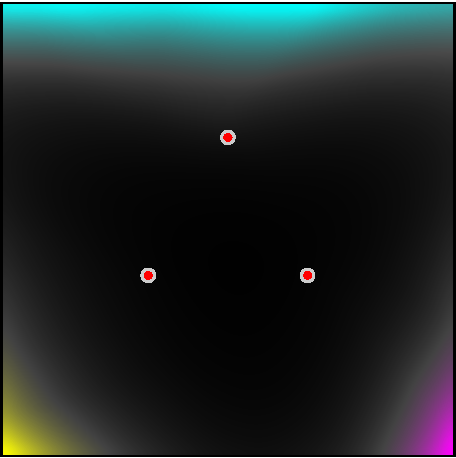
\includegraphics[width=0.5 \textwidth]{sections/006_neurips2020/figures/three_gaussians_no_flow-crop.pdf}
        \caption{\PostNetacro: \NoFlow}
    \end{subfigure}%   
    \begin{subfigure}[t]{0.33 \textwidth}
        \centering
        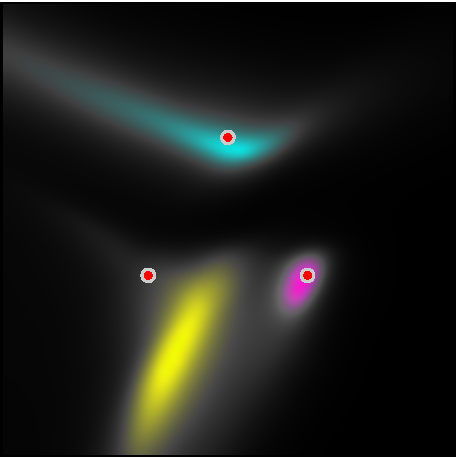
\includegraphics[width=0.5 \textwidth]{sections/006_neurips2020/figures/three_gaussians_no_UCE-crop.pdf}
        \caption{\PostNetacro: \NoUCE}
    \end{subfigure}%   
    \begin{subfigure}[t]{0.33 \textwidth}
        \centering
        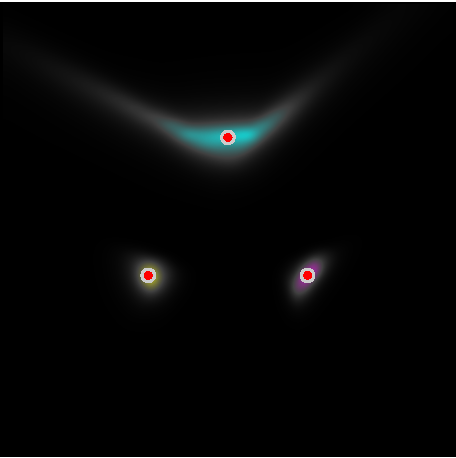
\includegraphics[width=0.5 \textwidth]{sections/006_neurips2020/figures/three_gaussians_normal-crop.pdf}
        \caption{\PostNetacro: Complete}
    \end{subfigure}%

    \caption{Uncertainty visualization for a 2D 3-Gaussians dataset. Red dots indicate the Gaussians means. Darker regions indicate high epistemic uncertainty for a class prediction. Ablated models fail even a simple dataset while \PostNetacro shows high certainty around gaussians means only.}
    \label{fig:toy_ablation}
	%\vspace{-.0cm}
\end{figure}

\begin{table}[H]
\resizebox{1 \textwidth}{!}{%
\begin{tabular}{lllllll}
\toprule
{} &  \textbf{Acc.} & \textbf{Alea. Conf.} & \textbf{Epist. Conf.}  & \textbf{Brier} & \textbf{OOD Alea.} & \textbf{OOD Epist.} \\
\midrule
\midrule
\textbf{PostN: No-Flow        } &  \cellcolor{Gray} 55.38$\pm$0.7 & \cellcolor{Gray} 85.46$\pm$0.3 & \cellcolor{Gray} 82.58$\pm$0.6 & \cellcolor{Gray} 64.4$\pm$0.6 & \cellcolor{Gray} 29.59$\pm$0.1 & \cellcolor{Gray} 31.15$\pm$0.4 \\
\textbf{PostN: No-Bayes-Loss} &   96.6$\pm$0.2 & 99.74$\pm$0.0 & 98.68$\pm$0.1 & \cellcolor{Gray} 8.85$\pm$0.4 & \cellcolor{Gray} 62.39$\pm$1.5 & \cellcolor{Gray} 82.63$\pm$1.4 \\
\textbf{PostN: Seq-No-Bn   } &  \cellcolor{Gray} 15.09$\pm$1.0 & \cellcolor{Gray} 39.88$\pm$7.2 &  \cellcolor{Gray}  39.86$\pm$7.2 &  \cellcolor{Gray} 89.88$\pm$1.3 & \cellcolor{Gray} 57.19$\pm$2.5 & \cellcolor{Gray} 56.74$\pm$2.4 \\
\textbf{PostN: Seq-Bn    } &  98.42$\pm$0.1 & 99.92$\pm$0.0 & 98.76$\pm$0.1 &   5.41$\pm$0.1 & \cellcolor{Gray} 52.35$\pm$0.7 &  \cellcolor{Gray} 71.75$\pm$1.9 \\
\bottomrule
\end{tabular}

    }
    \caption{Ablation study results on Sensorless Drive dataset. Gray cells indicate significant drops in scores compared to complete \PostNetacro Rad. in \cref{fig:unc_sensorless_drive}.}
        \label{fig:ablation_sensorless_drive}
    % \vspace{-.5cm}
\end{table}

We performed an ablation study on each component of \PostNetacro to evaluate their individual contributions. We were especially interested in comparing stability and uncertainty estimates. Thus, we removed independently the normalizing flow component (\NoFlow) and the novel Bayesian loss (\NoUCE) replaced by the classic cross-entropy loss. Furthermore, we used pre-trained models and subsequently only trained the normalizing flow component, with or without a batch normalization layer (\SeqBn and \SeqNoBn). We report results in \cref{fig:ablation_sensorless_drive}. \NoFlow has a significant drop in OOD detection scores similarly to Prior Networks; not surprising since they mainly differ by their loss. This underlines the importance of using normalized density estimation to differentiate ID and OOD data. The lower performance of \NoUCE compared to the original model indicates the benefit of using our Bayesian loss.
 \SeqBn obtains good performance for some of the metrics, which as a by-product, allows to estimate uncertainty on pre-trained models. Though, we noticed better performance for joint training in general. As shown by \SeqNoBn scores, the batch normalization layer brings stability. It intuitively facilitates predicted latent positions to lie on non-zero density regions. Similar conclusions can be drawn on the toy dataset (see \cref{fig:toy_ablation}) and the Segment dataset (see \cref{sec:app_additional_results}). We further compare various density types and latent dimensions in appendix. We noticed that a too high latent dimension leads to a performance decrease. We also observed that flow-based density estimation generally achieves better scores.

\begin{table}[H]
    \resizebox{1 \textwidth}{!}{%
\begin{tabular}{lllllllll}
\toprule
{} & \textbf{OOD K.} & \textbf{OOD K.} & \textbf{OOD F.} & \textbf{OOD F.} & \textbf{OODom K.} & \textbf{OODom K.} & \textbf{OODom F.} & \textbf{OODom F.} \\
{} & \textbf{Alea.} & \textbf{Epist.} & \textbf{Alea.} & \textbf{Epist.} & \textbf{Alea.} & \textbf{Epist.} & \textbf{Alea.} & \textbf{Epist.} \\
\midrule
\midrule
\textbf{RKL-PN      } &         60.76$\pm$2.9 &          53.76$\pm$3.4 &         78.45$\pm$3.1 &          72.18$\pm$3.6 &            9.35$\pm$0.1 &             8.94$\pm$0.0 &            9.53$\pm$0.1 &             8.96$\pm$0.0 \\
\textbf{RKL-PN w/ F.} &         81.34$\pm$4.5 &          78.07$\pm$4.8 &         \textbf{100.0$\pm$0.0} &          \textbf{100.0$\pm$0.0} &            9.24$\pm$0.1 &             9.08$\pm$0.1 &           88.96$\pm$4.4 &            87.49$\pm$5.0 \\
\textbf{PostN       } &         \textbf{95.75$\pm$0.2} &          \textbf{94.59$\pm$0.3} &         97.78$\pm$0.2 &          97.24$\pm$0.3 &           \textbf{100.0$\pm$0.0} &            \textbf{100.0$\pm$0.0} &           \textbf{100.0$\pm$0.0} &            \textbf{100.0$\pm$0.0} \\
\bottomrule
\end{tabular}

    }
    \caption{Results on MNIST for OOD detection against KMNIST (K.) and FashionMNIST (F.). We trained Rev. KL divergence PriorNets with uniform noise (RKL-PN) and Fashion MNIST (RKL-PN w/ F.) as OOD. \PostNetacro requires no OOD data. Larger numbers are better.}
    \label{fig:unc_MNIST}
    % \vspace{-.5cm}
\end{table}

Results of the comparison between RKL-PN, RKL-PN w/ F and \PostNetacro for OOD detection on MNIST are shown in \cref{fig:unc_MNIST}. Not surprisingly, the usage of FashionMNIST as OOD data for training helped RKL-PN to detect other FashionMNIST data. Except for FashionMNIST OOD, \PostNetacro still outperforms RKL-PN w/ F. in OOD detection for other datasets. We noticed that tabular datasets, defined on an unbounded input domain, are more difficult for baselines. One explanation is that due to the $\min$/$\max$ normalization it can happen that test samples lie outside the interval $[0,1]$ observed during training. For images, the input domain is compact, which allows to define a valid distribution for OOD data (e.g. uniform) which makes OODom data challenging (see OOD vs OODom in \cref{fig:unc_MNIST}).

\begin{table}[H]
    \resizebox{1 \textwidth}{!}{%
\begin{tabular}{lllllllll}
\toprule
{} &  \textbf{Acc.} & \textbf{Alea. Conf.} & \textbf{Epist. Conf.}  & \textbf{Brier} & \textbf{OOD Alea.} & \textbf{OOD Epist.} & \textbf{OODom Alea.} & \textbf{OODom Epist.} \\
\midrule
\midrule
\textbf{Drop Out C.} &  71.73$\pm$0.2 &        92.18$\pm$0.1 &          84.38$\pm$0.3 &  49.76$\pm$0.2 &      \textbf{72.94$\pm$0.3} &       41.68$\pm$0.5 &         28.3$\pm$1.8 &          47.1$\pm$3.3 \\
\textbf{KL-PN C.   } &  48.84$\pm$0.5 &        78.01$\pm$0.6 &          77.99$\pm$0.7 &  83.11$\pm$0.6 &      59.32$\pm$1.1 &       58.03$\pm$0.8 &        17.79$\pm$0.0 &         20.25$\pm$0.2 \\
\textbf{RKL-PN C.  } &  62.91$\pm$0.3 &        85.62$\pm$0.2 &          81.73$\pm$0.2 &  58.12$\pm$0.4 &      67.07$\pm$0.4 &       56.64$\pm$0.8 &        17.83$\pm$0.0 &         17.76$\pm$0.0 \\
\textbf{PostN C.   } &  \textbf{76.46$\pm$0.3} &        \textbf{94.75$\pm$0.1} &          \textbf{94.34$\pm$0.1} &  \textbf{37.39$\pm$0.4} &      72.83$\pm$0.6 &       \textbf{72.82$\pm$0.7} &        \textbf{100.0$\pm$0.0} &         \textbf{100.0$\pm$0.0} \\
\midrule
\textbf{Drop Out V.} &  82.84$\pm$0.1 &        97.15$\pm$0.0 &           96.6$\pm$0.0 &  27.15$\pm$0.2 &      51.39$\pm$0.1 &       53.64$\pm$0.1 &        51.38$\pm$0.1 &         53.66$\pm$0.1 \\
\textbf{KL-PN V.   } &  27.46$\pm$1.7 &        50.61$\pm$4.0 &          52.49$\pm$4.2 &  87.28$\pm$1.0 &      43.96$\pm$1.9 &       43.23$\pm$2.3 &        18.14$\pm$0.1 &         19.12$\pm$0.4 \\
\textbf{RKL-PN V.  } &  64.76$\pm$0.3 &        86.11$\pm$0.4 &          85.59$\pm$0.3 &  54.73$\pm$0.4 &      53.61$\pm$1.1 &       49.37$\pm$0.8 &        29.07$\pm$2.1 &         24.84$\pm$1.3 \\
\textbf{PostN V.   } &  \textbf{84.85$\pm$0.0} &        \textbf{97.76$\pm$0.0} &          \textbf{97.25$\pm$0.0} &  \textbf{22.84$\pm$0.0} &      \textbf{80.21$\pm$0.2} &       \textbf{77.71$\pm$0.3} &        \textbf{91.35$\pm$0.5} &         \textbf{99.25$\pm$0.1} \\
\bottomrule
\end{tabular}

    }
    \caption{Results on CIFAR10 with simple convolutional architectures (C.) and VGG16 (V.). Bold numbers indicate best score among one architecture type.}
    \label{fig:unc_CIFAR10}
    % \vspace{-.5cm}
\end{table}

Uncertainty estimation should be good regardless of the model accuracy. It is even more important for less accurate models since they actually \emph{do not know} (i.e.\ they do more mistakes). Thus, we compared the models that use a single network for training (using a convolutional architecture and VGG16) in \cref{fig:unc_CIFAR10}. Without the knowledge of true OOD data (SVHN) during training, Prior Networks struggle to achieve good performance. In contrast, \PostNetacro outputs high quality uncertainty estimates regardless of the architecture used for the encoder. We report additional results for PostNet using other encoder architectures (convolutional architecture, AlexNet \cite{alexnet}, VGG \cite{vgg} and ResNet \cite{resnet}) in \cref{tab:architecture_CIFAR10}. Deep generative models as Glow \cite{glow} using density estimation on input space are unable to distinguish between CIFAR10 and SVHN \cite{deep-generative}. In contrast, \PostNetacro clearly distinguishes between in-distribution data (CIFAR10) with low entropy, out-of-distribution (OOD SVHN) with high entropy, and close to the maximum possible entropy for out-of-domain data (OODom SVHN) (see \cref{cifar_shifts}a). Similar conclusions hold for MNIST and FashionMNIST (see \cref{sec:app_additional_results}). Furthermore, results for the image perturbations on CIFAR10 introduced by \cite{benchmarking-corruptions} are presented in \cref{cifar_shifts}.  We define the average change in confidence as the ratio between the average confidence \smash{$\frac{1}{N}\sum_i^{N}\alpha_0\dataix$} at severity 1 vs other severity levels. As larger shifts correspond to larger differences in the underlying distributions, we expect uncertainty-aware models to become less certain for more severe perturbations. \PostNet exhibits, as desired, the largest decrease in confidence with stronger corruptions (see \cref{cifar_shifts}b) while maintaining a high accuracy (see \cref{cifar_shifts}c).

\begin{table}[ht]
    \resizebox{1 \textwidth}{!}{%
\begin{tabular}{lllllllll}
\toprule
{} &  \textbf{Acc.} & \textbf{Alea. Conf.} & \textbf{Epist. Conf.}  & \textbf{Brier} & \textbf{OOD Alea.} & \textbf{OOD Epist.} & \textbf{OODom Alea.} & \textbf{OODom Epist.} \\
\midrule
\textbf{\PostNetacro: Conv.  } &  78.58$\pm$0.1 &        95.45$\pm$0.0 &          93.36$\pm$0.0 &  33.84$\pm$0.2 &      72.21$\pm$0.1 &       57.72$\pm$0.7 &        100.0$\pm$0.0 &         100.0$\pm$0.0 \\
\textbf{\PostNetacro: Alexnet} &  80.81$\pm$0.2 &        96.33$\pm$0.1 &          95.35$\pm$0.1 &  29.99$\pm$0.3 &       73.4$\pm$0.7 &       67.05$\pm$0.6 &        97.64$\pm$0.4 &         99.64$\pm$0.1 \\
\textbf{\PostNetacro: VGG    } &  84.85$\pm$0.0 &        97.76$\pm$0.0 &          97.25$\pm$0.0 & 22.84$\pm$0.0 &      80.21$\pm$0.2 &       77.71$\pm$0.3 &        91.35$\pm$0.5 &         99.25$\pm$0.1 \\
\textbf{\PostNetacro: Resnet } &  87.86$\pm$0.2 &        98.35$\pm$0.0 &          97.13$\pm$0.0 &  19.33$\pm$0.3 &      79.92$\pm$0.4 &       72.25$\pm$0.6 &        99.94$\pm$0.0 &         99.94$\pm$0.0 \\
\bottomrule
\end{tabular}

    }
    \caption{Results of \PostNetacro with different encoder architectures. It shows good uncertainty estimation regardless of the architecture complexity.}
    \label{tab:architecture_CIFAR10}
\end{table}

\begin{figure}[H]
    % \vspace{-.5cm}
    \centering
    \begin{subfigure}[t]{0.33 \textwidth}
        \centering
        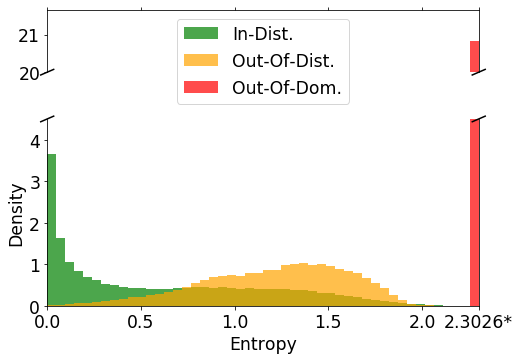
\includegraphics[width=.98 \textwidth]{sections/006_neurips2020/figures/entropy_CIFAR10.png}
        \caption{ID/OOD/OODom entropy}
    \end{subfigure}%  
    \begin{subfigure}[t]{0.33 \textwidth}
        \centering
        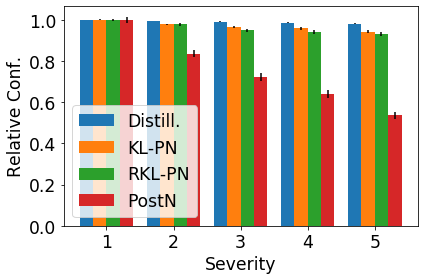
\includegraphics[width=.98 \textwidth]{sections/006_neurips2020/figures/shifts_CIFAR10_conf.png}
        \caption{Confidence under data shifts}
    \end{subfigure}%   
    \begin{subfigure}[t]{0.33 \textwidth}
        \centering
        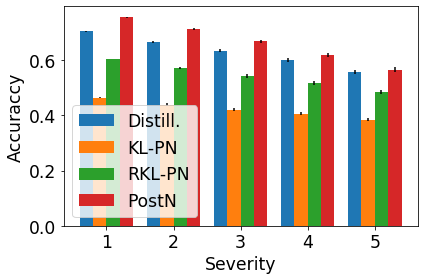
\includegraphics[width=.98 \textwidth]{sections/006_neurips2020/figures/shifts_CIFAR10_acc.png}
        \caption{Accuracy under data shifts}
    \end{subfigure}%   
    \caption{(a) shows entropy of the aleatoric distributions predicted by \PostNetacro on CIFAR10 (ID) and SVHN (OOD, OODom). The value $2.3026^*$ denotes the highest achievable entropy for 10 classes. \PostNetacro can easily distinguish between the three data types. (b) and (c) present averaged confidence and accuracy under 15 dataset shifts introduced by \cite{benchmarking-corruptions} on CIFAR10 with conv. architecture. On more severe perturbations (i.e. data further away from data distribution), \PostNetacro assigns higher epistemic uncertainty as desired. Baselines keeps same confidence even for less accurate predictions.}
    \label{cifar_shifts}
    %\vspace{-.5cm}
\end{figure}
\section{Conclusion}
\label{sec:conclusion_006}

We propose \ours, a model for uncertainty estimation in classification without requiring out-of-distribution samples for training or costly sampling for uncertainty estimation. \oursacro is composed of three main components: an encoder which outputs a position in a latent space, a normalizing flow which performs a density estimation in this latent space, and a Bayesian loss for uncertainty-aware training. In our extensive experimental evaluation, \oursacro achieves state-of-the-art performance with a strong improvement for detection of in- and out-of-distribution samples.

% \section*{Retrospective}
% \addcontentsline{toc}{section}{\protect Retrospective}%
\chapter{Uncertainty Estimation for Regression}
\label{chap:regression}

\section{Introduction}

\begin{wrapfigure}{r}{0.45\textwidth}
\vspace{-6mm}
	\centering
	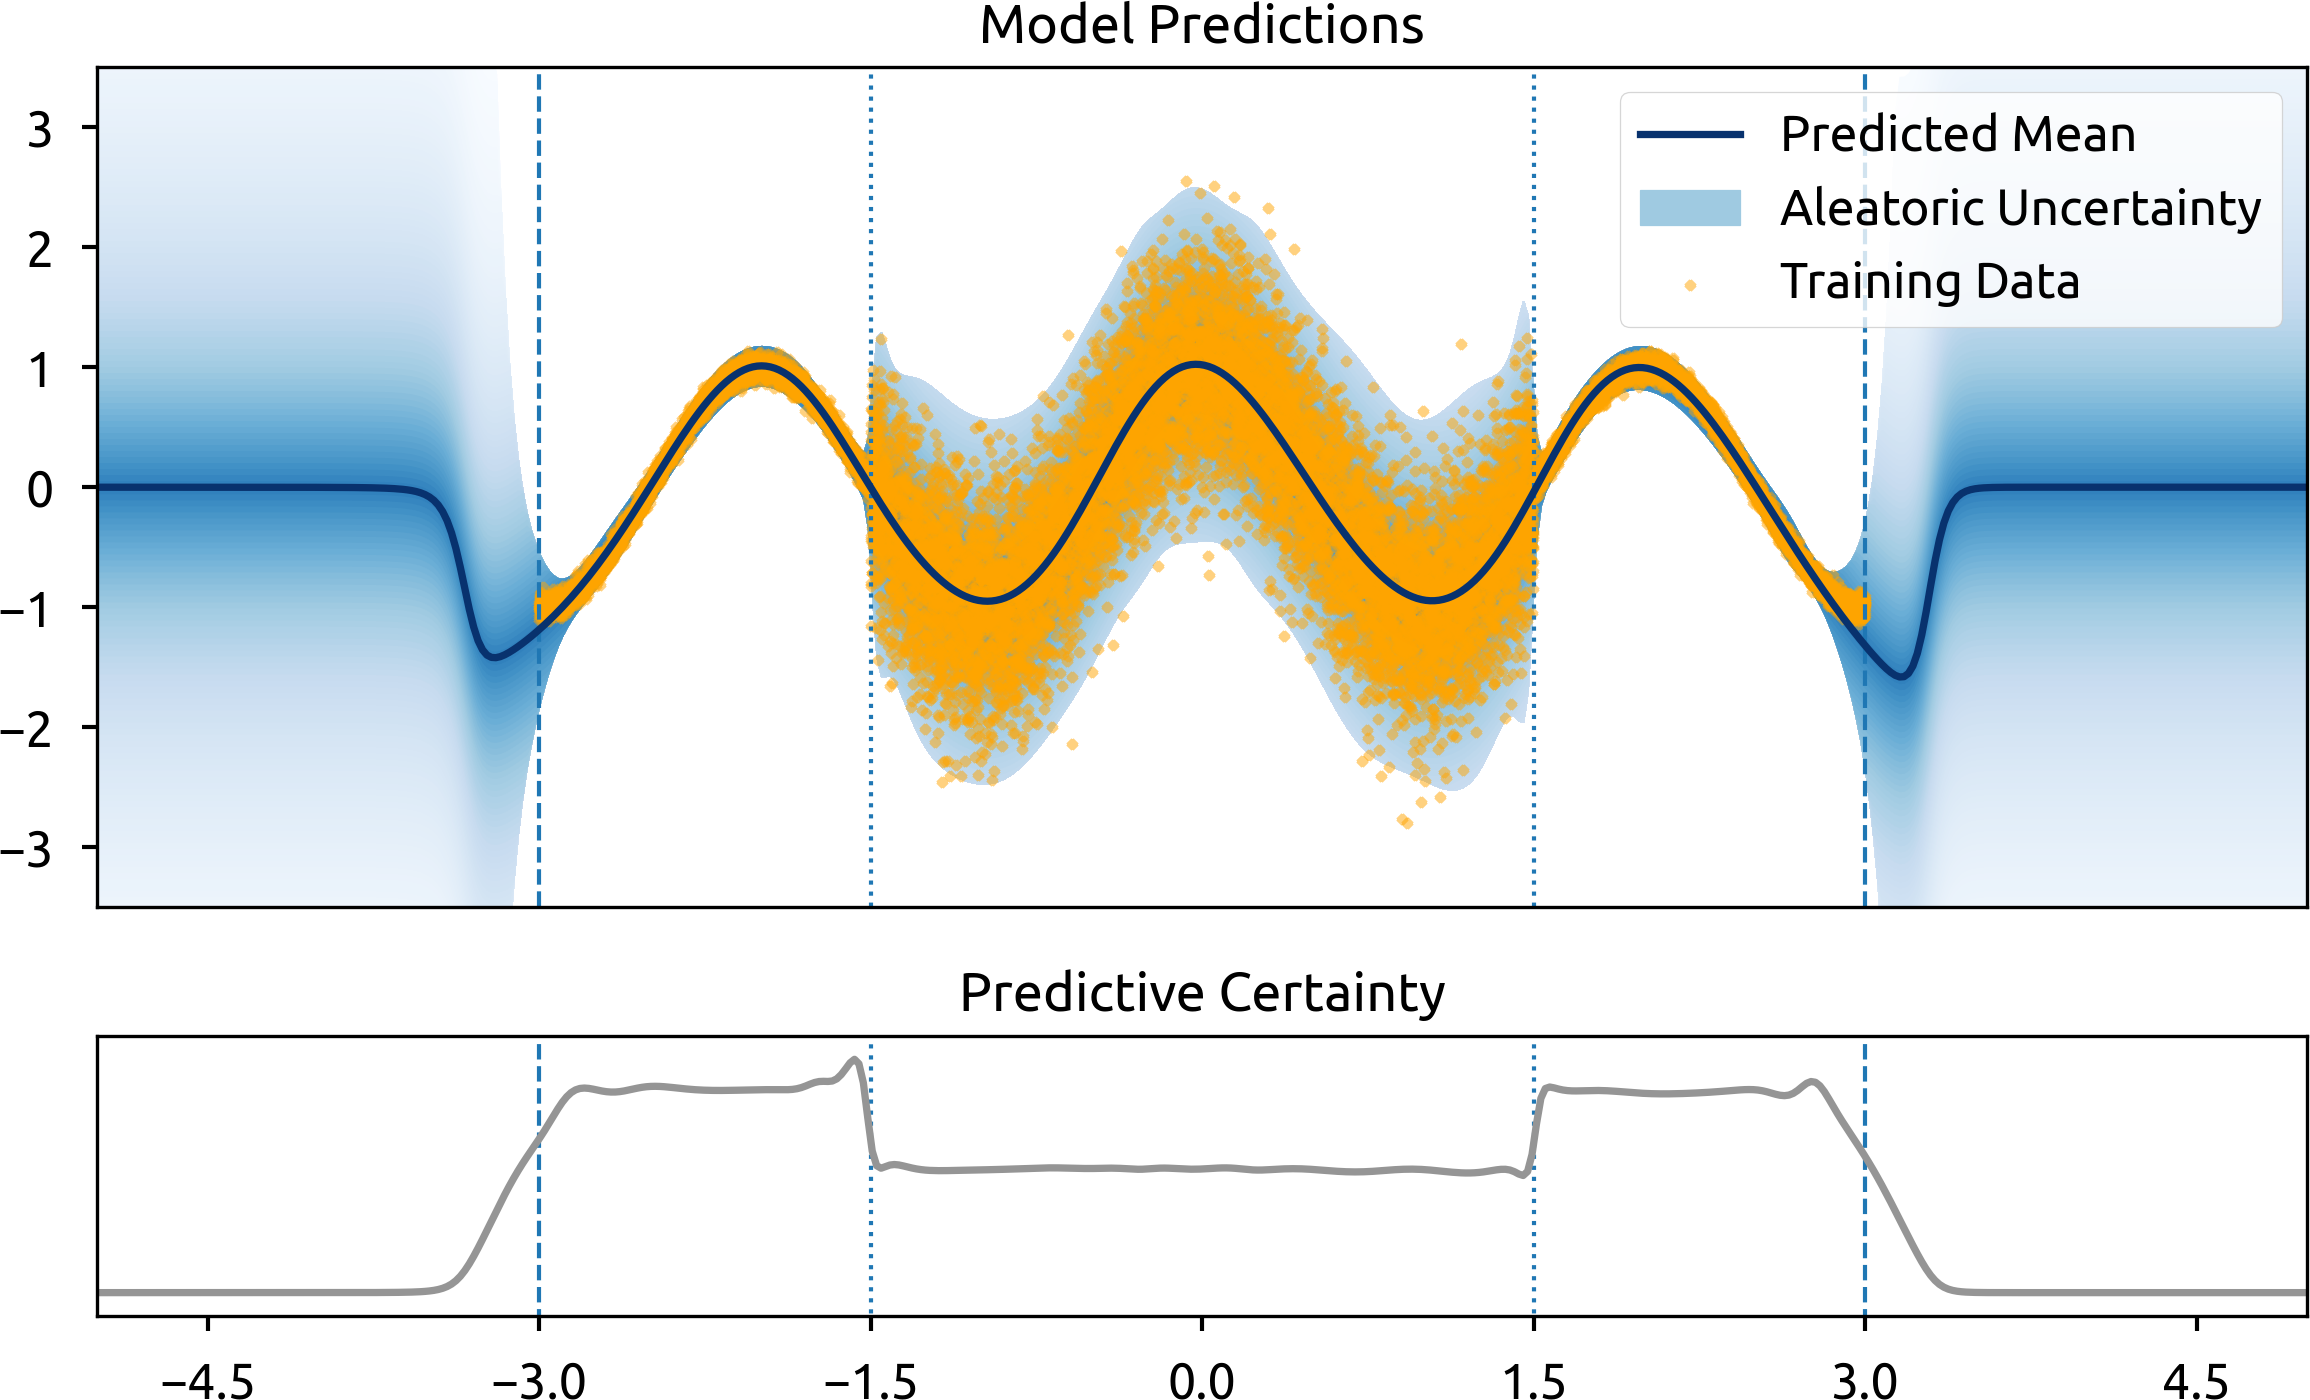
\includegraphics[width=0.42\textwidth]{sections/007_iclr2022/resources/toy-regression-trimmed.png}
    \caption*{Toy Regression Task}
    \vspace{0.3cm}
    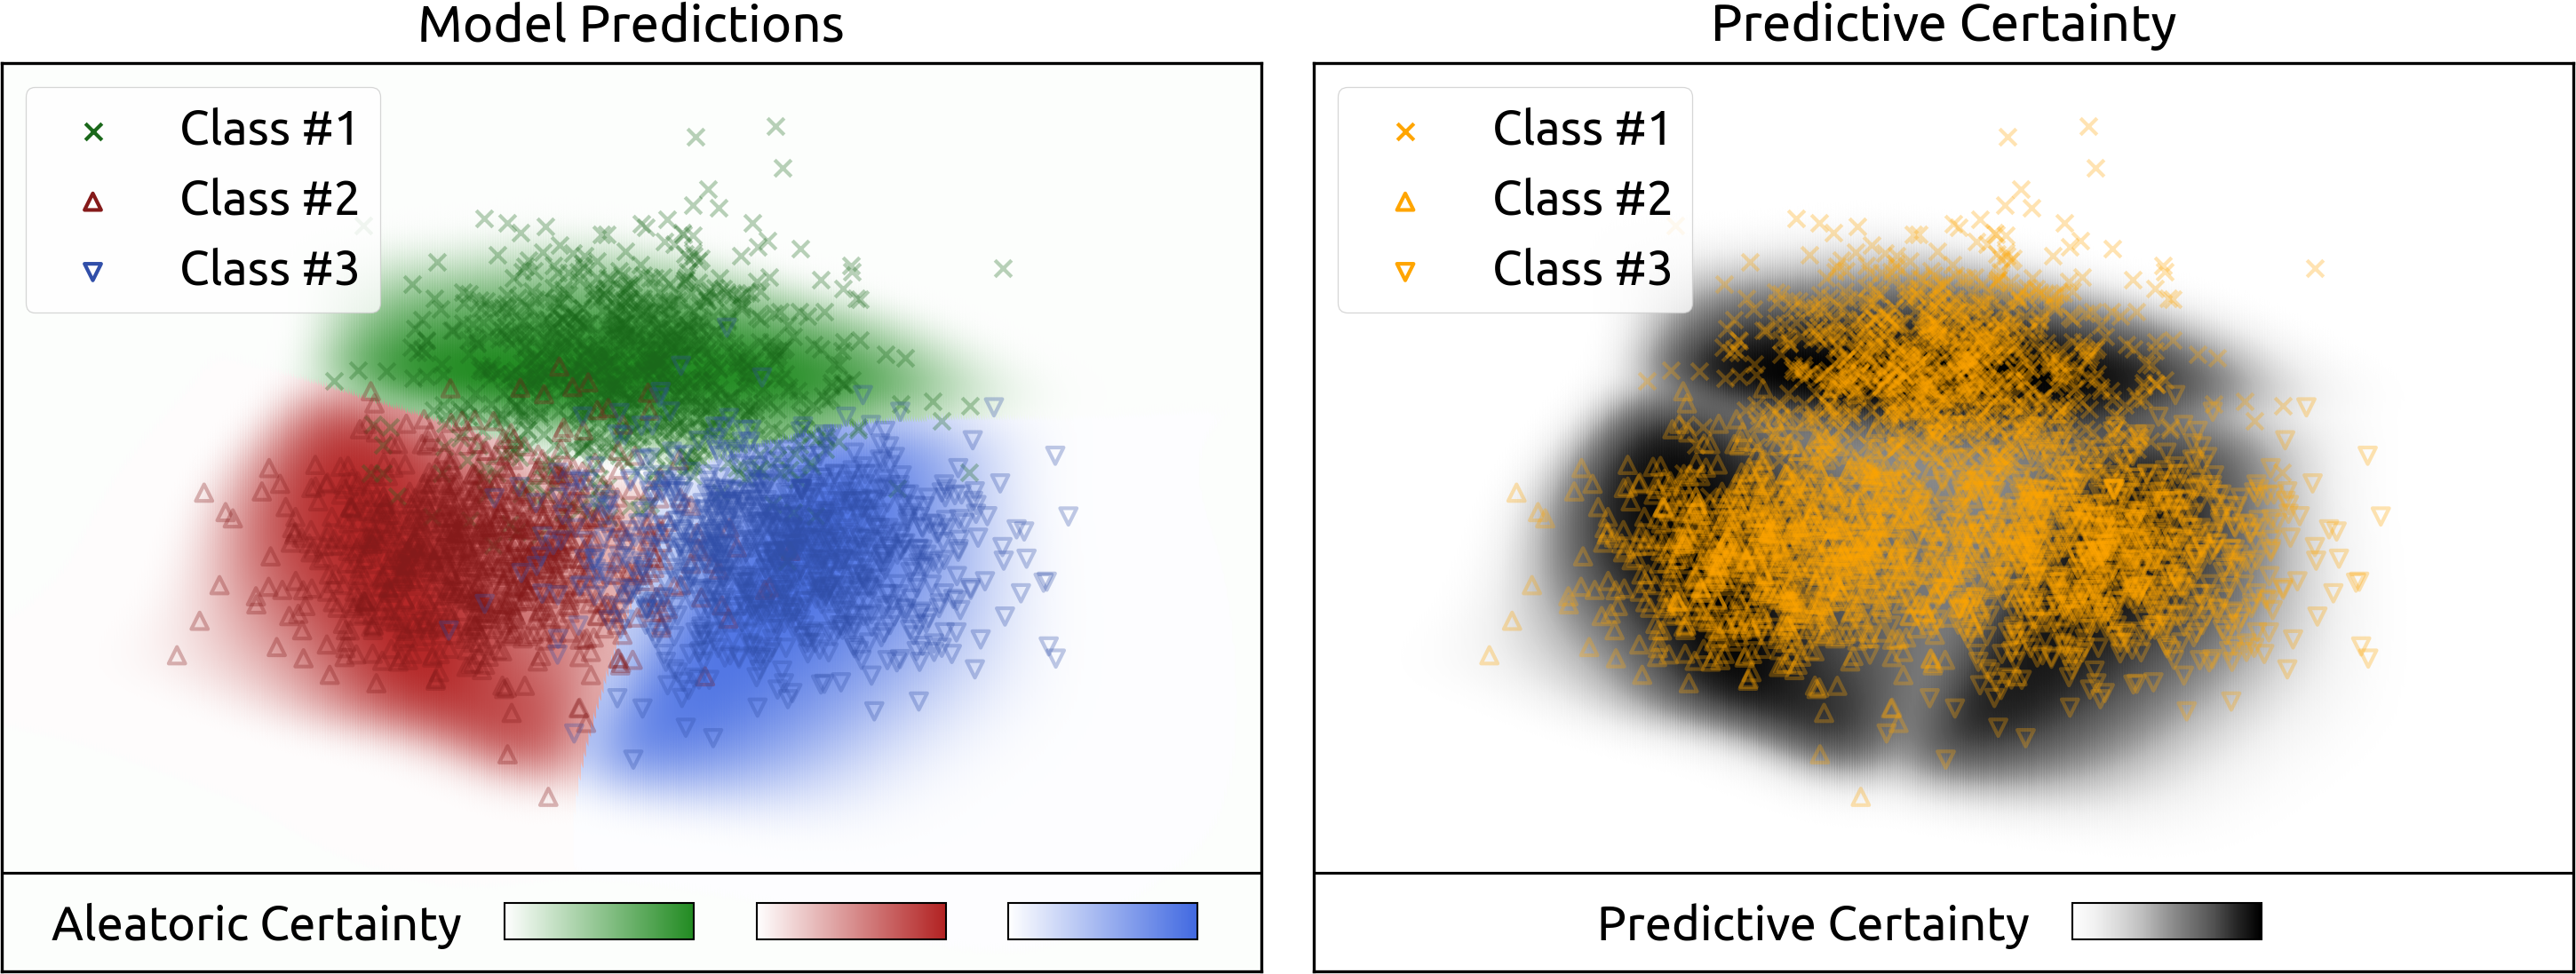
\includegraphics[width=0.42\textwidth]{sections/007_iclr2022/resources/toy-classification-trimmed.png}
    \caption*{Toy Classification Task}
    \caption{Visualization of the aleatoric and predictive uncertainty estimates of \NatPNacro{} on two toy regressions and classification tasks. \NatPNacro{} correctly assigns higher uncertainty to regions far from the training data.}
    \label{fig:toy-example-uncertainty}
    \vspace{-6mm}
\end{wrapfigure}

Accurate and rigorous uncertainty estimation is key for reliable machine learning models in safety-critical domains. It quantifies the confidence of machine learning models, thus allowing them to validate knowledgeable predictions corresponding to correct/wrong predictions, flag predictions on unknown input domains corresponding to anomaly or Out-of-Distribution detection, or detect natural shifts of the data facilitating real-time model maintenance \citep{dataset-shift, shifts-dataset, comparison-bayesian-diabetic}. Specifically, a reliable model can handle all these failure modes with high-quality estimates of \emph{aleatoric} and \emph{epistemic} uncertainty \citep{uncertainty-deep-learning}. These two levels of uncertainty allow a model to account for both irreducible data uncertainty (e.g. a fair dice's chance of $1/6$ for each face) and uncertainty due to the lack of knowledge about unseen data (e.g. input features differing significantly from training data or a covariate shift) respectively. Aleatoric and epistemic uncertainty levels can eventually be combined into an overall \emph{predictive uncertainty} \citep{uncertainty-deep-learning}

Traditional neural networks are not readily applicable in safety-critical domains as they show overconfident prediction, in particular on data that is different from training data \citep{calibration-network, ensembles}. To mitigate this problem, an important model family for uncertainty estimation directly predicts the parameters of a \emph{conjugate prior distribution} on the predicted \emph{target probability distribution}, thus accounting for the different levels of uncertainty. These models are efficient as they only require \emph{a single forward pass} for target and uncertainty prediction. Most of those models focus on classification and thus predict parameters of a Dirichlet distribution \citep{uceloss,postnet,priornet,reverse-kl,max_gap_id_ood,uncertainty-generative-classifier,multifaceted_uncertainty,graph_posterior,graph_uncertainty, lightweight-prob-net}. However, only two works \citep{evidential-regression, regression-priornet} have focused on regression by learning parameters of a Normal Inverse-Gamma (NIG) distribution as conjugate prior. Hence, all these models are limited to a \emph{single} task (e.g. either classification or regression). Some approaches even require out-of-distribution (OOD) data at training time \citep{priornet, reverse-kl} which is an unrealistic assumption in many real-world applications where anomalies are a priori diverse, rare or unknown.

\textbf{Our contribution.} We propose \NatPN{} (\NatPNacro{}) as a new approach parametrizing conjugate prior distributions for versatile uncertainty estimation. \NatPNacro{}{} is motivated from both the theoretical and practical perspective. 
\textbf{(1)} \NatPNacro{} can estimate predictive uncertainty for \emph{any} task described by the general group of exponential family distributions contrary to existing approaches from this family of models. Notably, this encompasses very common tasks such as classification, regression and count prediction which can be described with Categorical, Normal and Poisson distributions, respectively. 
\textbf{(2)} In theory, \NatPNacro{} is based on a \emph{new unified exponential family framework} which performs an input-dependent Bayesian update. For every input, it predicts the parameters of the posterior over the target exponential family distribution. We show that this Bayesian update is \emph{guaranteed} to predict high uncertainty far from training data.
\textbf{(3)} In practice, \NatPNacro{} requires \emph{no OOD data for training}, only adds \emph{a single normalizing flow} density to the last predictor layer and provides fast uncertainty estimation in a \emph{single forward pass}. Our extensive experiments showcase the high performances of \NatPNacro{} for various criteria (accuracy, calibration, OOD and shift detection) and tasks (classification, regression and count prediction). We illustrate the accurate aleatoric and predictive uncertainty predictions of \NatPNacro{} on two toy examples for classification and regression in Fig.~\ref{fig:toy-example-uncertainty}. \emph{None of the conjugate prior related works} have similar theoretical and practical properties.

%flexible, sound, simple, high quality, fast

\section{Related Work}
\label{sec:related_work_007}

In this section, we describe other work related to uncertainty estimation for supervised learning. We refer to \citet{uncertainty-survey} for a detailed survey on uncertainty estimation in deep learning. 

\textbf{Sampling-based methods.} A first family of models estimates uncertainty by aggregating statistics (e.g. mean and variance) from different samples of an implicit predictive distribution. Examples are ensemble \citep{bayesian-classifier-combination,ensembles, dynamic-bayesian-combination-classifiers,batch-ensembles,hyper-ensembles} and dropout \citep{dropout} models which provide high-quality uncertainty estimates \citep{dataset-shift} at the cost of an
expensive sampling phase at inference time. Moreover, ensembles usually require training multiple models. Further, Bayesian neural networks (BNN) \citep{bayesian-networks, scalable-laplace-bnn, simple-baseline-uncertainty} model the uncertainty on the weights and also require multiple samples to estimate the uncertainty on the final prediction. While recent BNNs have shown reasonably good performance \citep{rank-1-bnn,practical-bayesian,liberty-depth-bnn}, modelling the distribution on the weights suffers from pathological behavior thus limiting these approaches in practice \citep{expressiveness-bnn, practical-bnn, what-bnn-posterior}. In particular, \citet{what-bnn-posterior} uses an enormous computation budget by parallelizing the computation over 512 TPUv3  devices and running tens of thousands of training epochs to achieve a more exact Bayesian inference which is not suitable for practical applications. In contrast, \NatPNacro{} predicts uncertainty in \emph{a single forward pass} with a \emph{closed-form posterior distribution} over the target variable. \NatPNacro{} \emph{does not} model uncertainty on the weights.

\textbf{Sampling-free methods.} A second family of models is capable of estimating uncertainty in a single forward pass. The family of models parametrizing conjugate prior distributions is the main focus of this paper \citep{survey_evidential_uncertainty,evaluating_dbu,max_gap_id_ood,uncertainty-generative-classifier,multifaceted_uncertainty,graph_posterior, lightweight-prob-net}. Beyond this family of models, we differentiate between four other families of sampling-free models for uncertainty estimation. A first family aims at learning deep Gaussian processes with random features projections or learned inducing points \citep{uncertainty-distance-awareness, due, duq, uceloss}. A second family aims at learning deep energy-based models \citep{ood_ebm, jem_ebm}. Another family of models aims at propagating uncertainty across layers \citep{natural-parameter-network, sampling-free-variance-propagation, feed-forward-propagation, lightweight-prob-net, probabilistic-backprop-scalable-bnn}. They model uncertainty at the weight and/or activation levels and are generally constrained to specific transformations. In contrast, \NatPNacro{} only models the uncertainty on the predicted target variable and does not enforce any constraint on the encoder architecture. Further, some of the models propagating uncertainty already used the exponential family framework \citep{natural-parameter-network, deep-exponential-families}. However, while they parametrize exponential family distributions, \NatPNacro{} parametrizes the \emph{conjugate prior of the target exponential family distributions} which accounts for the epistemic uncertainty. Finally, while the family of calibration models aims at calibrating predictions \citep{accurate-uncertainties-deep-learning-regression, confidence-aware-learning, individual-calibration, distribution-calibration-regression, intra-order-preserving}, \NatPNacro{} aims at accurately modelling both aleatoric and epistemic uncertainty on in- and out-of-distribution data.

\section{Natural Posterior Network}
\label{sec:model_007}

At the very core of \NatPNacro{} stands the Bayesian update rule: $    \prior(\expparam \condition \mathcal{D}) \propto \prob(\mathcal{D} \condition \expparam) \times \prior(\expparam)$
%
%\begin{equation}\label{eq:general-bayesian-update}
%    \prior(\expparam \condition \mathcal{D}) \propto \prob(\mathcal{D} \condition \expparam) \times \prior(\expparam)
%\end{equation}
%
where $\prob(\mathcal{D} \condition \expparam)$ is the target distribution of the target data $\mathcal{D}$ given its parameter $\expparam$, and $\prior(\expparam )$ and $\prior(\expparam \condition \mathcal{D})$ are the prior and posterior distributions, respectively, over the target distribution parameters. The target distribution $\prob(\mathcal{D} \condition \expparam)$ could be any likelihood describing the observed target labels. The Bayesian update has three main advantages: \textbf{(1)} it introduces a prior belief which represents the safe default prediction if no data is observed, \textbf{(2)} it updates the prior prediction based on observed target labels, and \textbf{(3)} it assigns a confidence for the new target prediction given the aggregated evidence count of observed target labels. While \NatPNacro{} is capable to perform a Bayesian update for every possible input given the observed training data, we first recall the Bayesian background for a single exponential family distribution.

\begin{table*}[ht!]
	\vspace{-3mm}
	\centering
	\resizebox{.89\textwidth}{!}{%
\begin{tabular}{lccl}
\toprule
\multicolumn{1}{c}{Likelihood $\prob$} & \multicolumn{1}{c}{Conjugate Prior $\prior$} & \multicolumn{1}{c}{Parametrization Mapping $m$} & \multicolumn{1}{c}{Bayesian Loss (Eq.~\ref{eq:bayesian-loss})}\\
\midrule
\midrule
$\y \sim \DCat(\bm{p})$ & 
$\bm{p} \sim \DDir(\bm{\alpha})$ & 
\begin{tabular}{@{}l@{}}
$\priorparam=\bm{\alpha}/\evidence$ \\
$\evidence=\sum_\iclass \alpha_\iclass$
\end{tabular} &
\begin{tabular}{@{}l@{}}
    \textbf{(i)} $= \psi(\alpha_{\y*}\dataix) - \psi(\alpha_0\dataix)$ \\
    \textbf{(ii)} $= \log B(\bm{\alpha}\dataix) + (\alpha_0\dataix - \nclass) \psi(\alpha_0\dataix) - \sum_\iclass (\alpha_\iclass\dataix - 1) \psi(\alpha_\iclass\dataix)$
\end{tabular} \\
\midrule
$\y \sim \DNormal(\mu, \sigma)$ & 
$\mu, \sigma \sim \DNIG(\mu_0, \lambda, \alpha, \beta)$ & 
\begin{tabular}{@{}l@{}}
$\priorparam=\begin{pmatrix}\mu_0 \\ \mu_0^2 + \frac{2\beta}{\evidence} \end{pmatrix}$\\
$\evidence = \lambda= 2 \alpha$
\end{tabular} &
\begin{tabular}{@{}l@{}}
    \textbf{(i)} $= \frac{1}{2}\left(- \frac{\alpha}{\beta} (\y - \mu_0)^2 - \frac{1}{\lambda} + \psi(\alpha) - \log{\beta} - \log{2\pi}\right)$ \\
    \textbf{(ii)} $= \frac{1}{2} + \log\left((2\pi)^{\frac{1}{2}}\beta^{\frac{3}{2}}\Gamma(\alpha)\right) - \frac{1}{2} \log{\lambda} + \alpha - (\alpha+\frac{3}{2})\psi(\alpha)$
\end{tabular}\\
\midrule
$\y \sim \DPoi(\lambda)$ &
$\lambda \sim \DGamma(\alpha, \beta)$ &
\begin{tabular}{@{}l@{}}
$\chi=\alpha/\evidence$ \\
$\evidence=\beta$
\end{tabular} &
\begin{tabular}{@{}l@{}}
    \textbf{(i)} $= (\psi(\alpha) - \log{\beta}) \y - \frac{\alpha}{\beta} - \sum_{k=1}^{\y} \log k$ \\
    \textbf{(ii)} $= \alpha + \log{\Gamma(\alpha)} - \log{\beta} + (1 - \alpha) \psi(\alpha)$
\end{tabular}\\
\bottomrule
\end{tabular}}
	\caption{Examples of Exponential Family Distributions where $\psi(x)$ and $B(x)$ denote Digamma and Beta function, respectively.}
	\label{tab:summary_exp_dist}
	\vspace{-3mm}
\end{table*}

\subsection{Exponential Family Distribution}
% \textbf{Exponential Family Distribution.} 
Distributions from the exponential family are very widely used and have favorable analytical properties. Indeed, \textbf{(1)} they cover a wide range of target variables like discrete, continuous, counts or spherical coordinates, and \textbf{(2)} they benefit from intuitive and generic formulae for their parameters, density functions and statistics which can often be evaluated in closed-form. Important examples of exponential family distributions are Normal, Categorical and Poisson distributions (see Tab.~\ref{tab:summary_exp_dist}). Formally, an exponential family distribution on a target variable $\y \in \real$ with \emph{natural parameters} $\expparam \in \real^\suffstatdim$ can be denoted as
%
\begin{equation}\label{eq:exponential-family}
    \prob(\y \condition \expparam) = h(\y) \exp\left(\expparam^T \bm{u}(\y) - A(\expparam)\right)
\end{equation}
%
where ${h: \real \rightarrow \real}$ is the \emph{carrier or base measure}, ${A: \real^\suffstatdim \rightarrow \real}$ the \emph{log-normalizer} and ${\bm{u}: \real \rightarrow \real^\suffstatdim}$ the \emph{sufficient statistics} \citep{bishop,exponential-entropy}. The entropy of an exponential family distribution can always be written as $\entropy[\prob] = A(\expparam) - \expparam^T \nabla_{\bm{\theta}}A(\expparam) - \expectation[\log{h(\y)}]$ \citep{exponential-entropy}.
An exponential family distribution always admits a conjugate prior, which often also is a member of the exponential family:
%
\begin{equation}\label{eq:prior}
    \prior(\expparam \condition \priorparam, \evidence) = \eta(\priorparam, \evidence) \exp\left( \evidence \, \bm{\theta}^T\priorparam  - \evidence A(\expparam) \right)
\end{equation}
%
where $\eta(\priorparam, \evidence)$ is a normalization coefficient, $\priorparam \in \real^L$ are \emph{prior parameters} and $\evidence \in \real^+$ is the \emph{evidence}. Given a set of $\ndata$ target observations $\{\y^{(i)}\}_{i}^{\ndata}$, it is easy to compute a closed-form Bayesian update $\prior(\expparam \condition \priorparam^\text{post}, \evidence^\text{post}) \propto \prob(\{\y^{(i)}\}_{i}^{\ndata} \condition \expparam) \times \prior(\expparam \condition \chi^\text{prior}, n^\text{prior})$:
%
\begin{equation}\label{eq:posterior}
    \prior(\expparam \condition \priorparam^\text{post}, \evidence^\text{post}) \propto \exp\left( \evidence^\text{post} \expparam^T\priorparam^\text{post} - \evidence^\text{post} A(\expparam) \right)
\end{equation}
%
where $\priorparam^\text{post}=\frac{\evidence^\text{prior} \priorparam^\text{prior}+ \sum_{j}^\ndata{\bm{u}(\y^{(j)})}}{\evidence^\text{prior} + \ndata}$ and $\evidence^\text{post}=\evidence^\text{prior} + \ndata$. We see that $\priorparam^{\text{prior}}$ (resp. $\priorparam^{\text{post}}$) can be viewed as the average sufficient statistics of $\evidence^{\text{prior}}$ (resp. $\evidence^{\text{post}}$) fictitious samples \citep{bishop}. 
Further, the average sufficient statistic of fictitious samples is equal to the expected sufficient statistic of the conjugate distribution, i.e. $\priorparam = \expectation_{\prior(\priorparam, \evidence)}[\expparam]$ \citep{exponential-family-stats, conjugate-prior-exponential-family}. Thus, the parameter $\priorparam^\text{post}$ carries the inherent aleatoric uncertainty on the target distribution with natural parameters $\expparam$, while the evidence $\evidence^\text{post}$ aligns well with the epistemic uncertainty (i.e. a low evidence means few prior target observations). We stress that the natural conjugate prior parametrization $\priorparam, \evidence$ is often different from the ``well-known'' parametrization $\bm{\kappa}$ used by standard coding libraries. By definition, a bijective mapping $m(\bm{\kappa}) = (\priorparam, \evidence)$ from the natural parametrization to the commonly used parametrization always exists (see examples in Tab.~\ref{tab:summary_exp_dist}). Finally, exponential family distributions always admit a closed-form posterior predictive distribution \citep{bayesian-data-analysis}.

\subsection{Input-Dependent Bayesian Update for Exponential Family Distributions}
%\textbf{Input-Dependent Bayesian Update for Exponential Family Distributions.} 
We propose to leverage the power of exponential family distributions for the more complex task when the prediction $\y\dataix$  depends on the input $\x\dataix$. Hence, \NatPNacro{} extends the Bayesian treatment of a single exponential family distribution prediction by predicting an individual posterior update per input. We distinguish between the chosen prior parameters $\priorparam^\text{prior}$, $\evidence^\text{prior}$ shared among samples, and the additional predicted parameters $\priorparam\dataix$, $\evidence\dataix$ dependent on the input $\x\dataix$ leading to the updated posterior parameters:
%
\begin{equation}\label{eq:parameter-update}
    \priorparam^{\text{post},(\idata)} = \frac{\evidence^\text{prior}\priorparam^\text{prior} + \evidence\dataix \priorparam\dataix}{\evidence^\text{prior} + \evidence\dataix}, \hspace{5mm}
    \evidence^{\text{post},(\idata)} = \evidence^\text{prior} + \evidence\dataix
\end{equation}
%
Equivalently, \NatPNacro{} may be interpreted as predicting a set of $\evidence\dataix$ pseudo observations $\{\y^{(j)}\}_{j}\dataix$ such that their aggregated sufficient statistics satisfy \smash{$\sum_{j}^{\evidence\dataix} \y^{(j)} = \evidence\dataix \priorparam\dataix$}, and perform the respective Bayesian update.
%
% \begin{equation}\label{eq:bayesian-update}
%     \begin{aligned}
% \prior(\expparam \condition \{\y^{(j)}\}_{j}\dataix) \propto \prob(\{\y^{(j)}\}_{j}\dataix \condition \expparam) \times \prior(\expparam)
%     \end{aligned}
% \end{equation}
%
This Bayesian update works for \emph{any} choice of exponential family distributions as long as parameters are mapped to their standard form (see Tab.~\ref{tab:summary_exp_dist}). According to the \emph{principle of maximum entropy} \citep{maximum-entropy-principle}, a practical choice for the prior is to enforce high entropy for the prior distribution which is usually considered less informative. It is typically achieved when the prior pseudo-count $\evidence^\text{prior}$ is small and the prior parameter $\priorparam^\text{prior}$ shows a high aleatoric uncertainty.

\begin{figure*}[t]
    \centering
    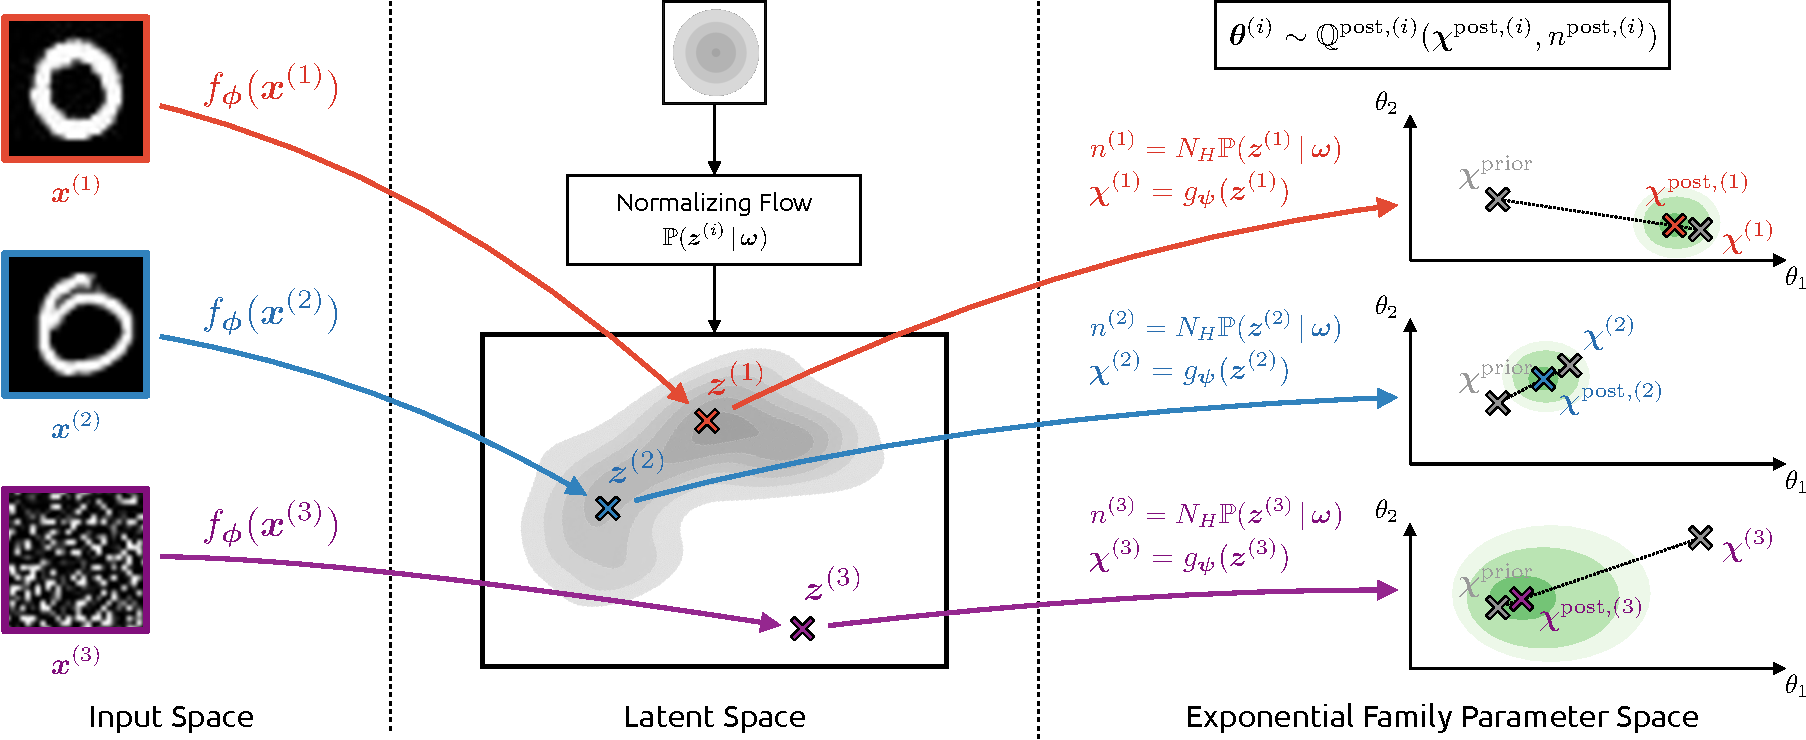
\includegraphics[width=.85\linewidth]{sections/007_iclr2022/resources/npn-crop.pdf}
    \caption{Overview of \NatPN{}. Inputs $\bm{x}^{(i)}$ are first mapped to a low-dimensional latent representation $\bm{z}^{(i)}$ by the encoder $f_{\bm{\phi}}$. From $\bm{z}^{(i)}$, the decoder $g_{\bm{\psi}}$ derives the parameter update $\bm{\chi}^{(i)}$ while a normalizing flow $\mathbb{P}_{\bm{\omega}}$ yields the evidence update $n^{(i)}$. Posterior parameters are obtained from a weighted combination of prior and update parameters according to $n^{\text{post},(i)}$.}
    \label{fig:npn}
    % \vspace{-1mm}
\end{figure*}

Hence, \NatPNacro{} proposes a generic way to perform the input-dependent Bayesian update $\priorparam\dataix$, $\evidence\dataix$ for \emph{any} exponential family distribution in three steps (see Fig.~\ref{fig:npn}): \textbf{(1)} An encoder $f_{\bm{\phi}}$ maps the input $\x\dataix$ onto a low-dimensional latent vector $\z\dataix = f_{\phi}(\x\dataix) \in \real^H$ representing useful features for the prediction task (see left Fig.\ref{fig:npn}). Note that the architecture of the encoder can be arbitrarily complex. Then, \textbf{(2)} the latent representation $\z\dataix$ is used in two different ways to predict the parameter update $\priorparam\dataix$ and the evidence update $\evidence\dataix$ (see center Fig.\ref{fig:npn}). On the one hand, a linear decoder $g_{\bm{\psi}}$ is trained to output the parameter update $\priorparam\dataix = g_{\bm{\psi}}(\z\dataix) \in \real^L$ accounting for the aleatoric uncertainty. On the other hand, a single normalized density is trained to output the evidence update $\evidence\dataix = N_H\prob(\z\dataix \condition \bm{\omega})$ accounting for the epistemic uncertainty. The intuition is that increasing the evidence on training data during training forces the evidence everywhere else (incl. far from training data) to decrease thanks to the density normalization constraint. The constant $N_H$ is a certainty budget distributed by the normalized density $\prob(\z\dataix \condition \bm{\omega})$ over the latent representations $\z\dataix$ i.e. $N_H = \int N_H \prob(\z\dataix \condition \bm{\omega}) d\z\dataix = \int \evidence\dataix d\z\dataix$. In practice, we observed that scaling the certainty budget w.r.t. the latent dimension $H$ helped the density to cover larger volumes in higher dimension (see app.). Finally, \textbf{(3)} \NatPNacro{} computes the posterior parameters $\priorparam^{\text{post}, (\idata)}$ and $\evidence^{\text{post}, (\idata)}$ which can be viewed respectively as the mean and concentration of the posterior distribution (see right Fig.\ref{fig:npn}). Note that the posterior parameter $\priorparam^{\text{post}, (\idata)}$ is a simple weighted average of the prior parameter $\priorparam^\text{prior}$ and the update parameter $\priorparam\dataix$ as shown by Eq.~\ref{eq:parameter-update}.

\NatPNacro{} extends PostNet \citep{postnet} which also performs an input-dependent Bayesian update with density estimation. Yet, it has three crucial differences which lead to major practical improvements. First, the new exponential family framework is significantly more flexible and is not restricted to classification. Second, the Dirichlet $\bm{\alpha}$ parameter computation is different: \NatPNacro{} computes the $\priorparam$ parameters -- which can be viewed as standard softmax output -- and the $\evidence$ evidence separately (i.e. $\bm{\alpha} = \evidence \priorparam$) while PostNet computes one evidence pseudo-count per class. Third, \NatPNacro{} is computationally more efficient. It requires a single density while PostNet requires $\nclass$ densities.

\subsection{ID and OOD Uncertainty Estimates}
%\textbf{ID and OOD Uncertainty Estimates.} 
\NatPNacro{} intuitively leads to reasonable uncertainty estimation for the two limit cases of strong in-distribution (ID) and out-of-distribution (OOD) inputs (see red and purple samples in Fig.~\ref{fig:npn}). For very likely \emph{in-distribution} data (i.e. $\prob(\z\dataix \condition \bm{\omega}) \rightarrow \infty$), the posterior parameter overrules the prior (i.e. $\priorparam^{\text{post}, (\idata)} \rightarrow \priorparam\dataix$). Conversely, for very unlikely \emph{out-of-distribution} data (i.e. $\prob(\z\dataix \condition \bm{\omega}) \rightarrow 0$), the prior parameter takes over in the posterior update (i.e. $\priorparam^{\text{post}, (\idata)} \rightarrow \priorparam^\text{prior}$). Hence, the choice of the prior parameter should reflect the default prediction when the model lacks knowledge. We formally show under mild assumptions on the encoder that \NatPNacro{} predicts very low additional evidence ($\evidence\dataix \approx 0$) for (almost) any input $\x\dataix$ far away from the training data (i.e. $||\x\dataix|| \rightarrow + \infty$), thus recovering prior predictions (i.e. $\priorparam^{\text{post}, (\idata)} \approx \priorparam^\text{prior}$) (see proof in app.).
\begin{theorem}
\label{thm:oodom-guarantee}
Let a \NatPNacro{} model be parametrized with a (deep) encoder $f_{\phi}$ with ReLU activations, a decoder $g_{\psi}$ and the density $\prob(\z \condition \bm{\omega})$. Let $f_{\phi}(\x)= V^{(l)}\x + a^{(l)}$ be the piecewise affine representation of the ReLU network $f_{\phi}$ on the finite number of affine regions $Q^{(l)}$ \citep{understanding-nn-relu}. Suppose that $V^{(l)}$ have independent rows and the density function $\prob(\z \condition \bm{\omega})$ has bounded derivatives, then for almost any $\x$ we have \smash{$\prob(f_{\phi}(\delta \cdot \x) \condition \bm{\omega}) \underset{\delta \rightarrow \infty}{\rightarrow} 0$}. i.e the evidence becomes small far from training data.
\end{theorem}
This theorem only requires that the density avoids very unlikely pathological behavior with unbounded derivatives \citep{limit-existence-infinity}. A slightly weaker conclusion holds using the notion of limit in density if the density function does not have bounded derivatives \citep{integrable-infinity}. Finally, the independent rows condition is realistic for trained networks with no constant output \citep{overconfident-relu}. It advantageously leads \NatPNacro{} to consistent uncertainty estimation contrary to standard ReLU networks which are overconfident far from training data \citep{overconfident-relu}.

\subsection{Bayesian \NatPNacro{} Ensemble} 
%\textbf{Bayesian \NatPNacro{} Ensemble.} 
Interestingly, it is natural to extend the Bayesian treatment of a single \NatPNacro{} to an ensemble of \NatPNacro{} models (NatPE). An ensemble of $m$ \NatPNacro{} models is intuitively equivalent to performing $m$ successive Bayesian updates using each \NatPNacro{} member separately. More formally, given an input $\x\dataix$ and an ensemble of $m$ jointly trained \NatPNacro{} models, the Bayesian update for the posterior distribution becomes ${\priorparam^{\text{post}, (\idata)} = \frac{\evidence^\text{prior}\priorparam^\text{prior} + \sum_k^{m} \evidence_k\dataix \priorparam_k\dataix}{\evidence^\text{prior} + \sum_k^{m} \evidence_k\dataix}}$ and ${\evidence^{\text{post}, (\idata)} = \evidence^\text{prior} + \sum_k^{m} \evidence_k\dataix}$. %which is equivalent to having observed $m$ sets of \smash{$\evidence_k\dataix$} pseudo observations. %$\{\y_k^{(j)}\}_{j}\dataix$ such that $\sum_{j}^{\evidence_m\dataix} \y^{(j)} = \priorparam_k\dataix$. 
Note that the standard Bayesian averaging which is used in many ensembling methods \citep{bayesian-ensemble-learning,ensembles,batch-ensembles,hyper-ensembles} is different from this Bayesian combination. While Bayesian averaging assume that only one model is correct, the Bayesian combination of \NatPNacro{} allows \emph{more} or \emph{none} of the models to be ``expert'' for some input  \citep{bayesian-averaging-to-combination}. For example, an input $\x\dataix$ unfamiliar to every model $m$ (i.e. $\evidence_m\dataix \approx 0$) would recover the prior default prediction $\priorparam^\text{prior}, \evidence^\text{prior}$. Existing models already had similar properties for Bayesian combination of classifiers \citep{bayesian-classifier-combination, dynamic-bayesian-combination-classifiers}.

\subsection{Optimization}
\label{sec:optimization}

The choice of the optimization procedure is of primary importance in order to obtain both high-quality target predictions and uncertainty estimates regardless of the task.

\paragraph{Bayesian Loss.} We follow \cite{postnet} and aim at minimizing the Bayesian formulation:
%
\begin{equation}\label{eq:bayesian-loss}
    \mathcal{L}\dataix = - \underbrace{\expectation_{\expparam\dataix \sim \prior^{\text{post},(\idata)}}[\log \prob(\y\dataix\condition \expparam \dataix)]}_\text{(i)} - \underbrace{\entropy[\prior^{\text{post},(\idata)}]}_\text{(ii)}
\end{equation}
%
where $\entropy[\prior^{\text{post},(\idata)}]$ denotes the entropy of the predicted posterior distribution $\prior^{\text{post},(\idata)}$. Similarly to the ELBO loss, this loss is guaranteed to be optimal when the predicted posterior distribution is close to the true posterior distribution $\prior^*(\expparam \condition \x\dataix)$ i.e. $\prior^{\text{post},(\idata)} \approx \prior^*(\expparam \condition \x\dataix)$ \citep{update-belief-propagation, PAC-bayesian_estimator, opt-info-processing_bayes}. However, this loss is generally \emph{not} equal to the ELBO loss especially for real valued targets i.e. $y \in \real$ (see app.). The term \textbf{(i)} is the expected likelihood under the predicted posterior distribution. It can be viewed as the Uncertain Cross Entropy (UCE) loss \citep{uceloss} which is known to reduce uncertainty on observed data. The term \textbf{(ii)} is an entropy regularizer acting as a prior which favors uninformative distributions $\prior^{\text{post},(\idata)}$ with high entropy. In our case, we assume the likelihood $\prob(\y\dataix\condition\expparam\dataix)$ and the posterior $\prior^{\text{post},(\idata)}$ to be members of the exponential family. We take advantage of the convenient computations for such distributions and derive a more explicit formula for the Bayesian formulation \eqref{eq:bayesian-loss} (see derivation in the appendix):
%
\begin{equation}\label{eq:nll-entropy}
    \begin{aligned}
    \mathcal{L}_\lambda\dataix &\propto \expectation[\expparam]^T \bm{u}(y\dataix) - \expectation[A(\bm{\expparam})] - \lambda\entropy[\prior^{\text{post},(\idata)}]
    \end{aligned}
\end{equation}
%
where $\lambda$ is an additional regularization weight tuned with a grid search. Note that the term $\expectation[\expparam]^T \bm{u}(y\dataix) $ favors a good alignment of the expected sufficient statistic $\expectation[\expparam] = \priorparam$ with the observed sufficient statistic $\bm{u}(y\dataix)$. In practice, all terms can be computed efficiently in closed form for most exponential family distributions (see examples in Tab.~\ref{tab:summary_exp_dist}). In particular, simplifications are possible when the conjugate prior distribution is also in an exponential family which is often the case. Ultimately Eq.~\eqref{eq:nll-entropy} applies to \emph{any} exponential family distribution unlike \cite{postnet}.

\textbf{Optimization Scheme.} \NatPNacro{} is fully differentiable using the closed-form Bayesian loss. Thus, we train the encoder $f_{\bm{\phi}}$, the parameter decoder $g_{\bm{\psi}}$ and the normalizing flow $\prob(\z\dataix \condition \bm{\omega})$ w.r.t. parameters $\bm{\phi}, \bm{\psi}, \bm{\omega}$ jointly. Further, we observed that ``warm-up training'' \citep{warm-start} and ``fine-tuning'' \citep{fine-tuning-continuous} of the density helped to improve uncertainty estimation for more complex flows and datasets. Thus, we train the normalizing flow density to maximize the likelihood of the latent representations before and after the joint optimization while keeping all other parameters fixed.

\subsection{Model Limitations} \label{sec:limitations}

\paragraph{Task-Specific OOD.} Previous works show that density estimation is unsuitable for acting on the raw image input \citep{anomaly-detection,deep-generative,typicality_OOD_generative} or on a non-carefully transformed space \citep{perfect-density-no-ood-guarantee}. To circumvent this issue, \NatPNacro{} does not perform OOD detection directly on the input but rather fits a normalizing flow on a learned space. In particular, the latent space is \textbf{(1)} low-dimensional, \textbf{(2)} task-specific and \textbf{(3)} encodes meaningful semantic features. Similarly, \cite{postnet, why-nf-fail-ood, density-states-ood, contrastive-ood} already improved OOD detection of density-based methods by leveraging a task-induced bias or low-dimensional statistics. In the case of \NatPNacro{}, the low-dimensional latent space has to contain relevant features to linearly predict the sufficient statistics required for the task. For example, \NatPNacro{} aims at a linearly separable latent space for classification. The downside is that \NatPNacro{} is capable of detecting OOD samples only with respect to the considered task and requires labeled examples during training. As an example, \NatPNacro{} likely fails to detect a change of image color if the task aims at classifying object shapes and the latent space has no notion of color. Hence, we underline that \NatPNacro{} comes with a task-dependent OOD definition, which is a reasonable choice in practice.

\paragraph{Model-Task Mismatch.} Second, we emphasize that the uncertainty estimation quality of \NatPNacro{} for (close to) ID data depends on the convergence of the model, the encoder architecture (e.g. MLP, Conv., DenseDepth \citep{dense-depth}) and the target distribution (e.g. Poisson, Normal distributions) choice which should match the task needs. However, we show \emph{empirically} that \NatPNacro{} provides high quality uncertainty estimates in practice on a wide range of tasks. Further, we show \emph{theoretically} that \NatPNacro{} leads to uncertain prediction far away from training data for \emph{any} exponential family target distributions. In comparison, \cite{provable-uncertainty} showed akin guarantees for classification only.
\section{Experiments}
\label{sec:experiments_007}

In this section, we compare \NatPNacro{} to existing methods on extensive experiments including three different tasks: classification, regression and count prediction. For each task type, we evaluate the prediction quality based on target error and uncertainty metrics. These various set-ups aim to highlight the versatility of \NatPNacro{}. In particular, \NatPNacro{} is the only model that adapts to all tasks and achieves high performances for all metrics without requiring multiple forward passes.

\begin{table*}[ht]
    \centering
    % \vspace{-1mm}
   % \scriptsize
   \caption{Classification results on Sensorless Drive with Categorical target distribution. Best scores among all single-pass models are in bold. Best scores among all models are starred.}
    \label{tab:sensorless-drive}
    % \vspace{-3mm}
    \resizebox{0.8 \textwidth}{!}{
    \begin{tabular}{lcccccc}
        \toprule
        & \textbf{Accuracy} & \textbf{Brier} & \textbf{9/10 Alea.} & \textbf{9/10 Epist.} & \textbf{OODom Alea.} & \textbf{OODom Epist.} \\
        \midrule
        \textbf{Dropout} & 98.62 $\pm$ 0.11 & 3.79 $\pm$ 0.29 & 30.20 $\pm$ 0.85 & 32.57 $\pm$ 1.45 & 27.03 $\pm$ 0.51 & 95.30 $\pm$ 1.66 \\
        \textbf{Ensemble} & 98.83 $\pm$ 0.17 & 3.00 $\pm$ 0.54 & 30.79 $\pm$ 0.74 & 32.61 $\pm$ 1.06 & 27.16 $\pm$ 0.59 & 99.97 $\pm$ 0.01 \\
        \textbf{NatPE} & *99.66 $\pm$ 0.03 & *0.68 $\pm$ 0.05 & 77.05 $\pm$ 1.93 & 83.73 $\pm$ 1.89 & 99.99 $\pm$ 0.00 & *100.00 $\pm$ 0.00 \\
        \midrule
        \textbf{R-PriorNet} & 98.85 $\pm$ 0.25 & 2.01 $\pm$ 0.47 & 40.13 $\pm$ 2.99 & 30.07 $\pm$ 0.81 & \textbf{*100.00 $\pm$ 0.00} & 23.59 $\pm$ 0.00 \\
        \textbf{EnD$^2$} & 93.95 $\pm$ 2.35 & 28.09 $\pm$ 6.40 & 26.35 $\pm$ 0.60 & 24.85 $\pm$ 0.43 & 84.43 $\pm$ 15.21 & 23.58 $\pm$ 0.00 \\
        \textbf{PostNet} & \textbf{99.64 $\pm$ 0.02} & \textbf{0.75 $\pm$ 0.08} & 80.60 $\pm$ 1.68 & \textbf{*92.57 $\pm$ 1.41} & \textbf{*100.00 $\pm$ 0.00} & \textbf{*100.00 $\pm$ 0.00} \\
        \textbf{\NatPNacro{}} & 99.61 $\pm$ 0.05 & 1.04 $\pm$ 0.29 & \textbf{*81.43 $\pm$ 1.89} & 79.54 $\pm$ 2.62 & 99.98 $\pm$ 0.00 & \textbf{*100.00 $\pm$ 0.00} \\
        \bottomrule
    \end{tabular}
    }
            % \vspace{-0mm}
\end{table*}

%\begin{table*}[ht]
%    \centering
%    \scriptsize
%    \resizebox{1.\textwidth}{!}{
%    \begin{tabular}{lcccccccc}
%        \toprule
%        & \textbf{Accuracy} & \textbf{Brier} & \textbf{K. Alea.} & \textbf{K. Epist.} & \textbf{F. Alea.} & \textbf{F. Epist.} & \textbf{OODom Alea.} & \textbf{OODom Epist.} \\
%        \midrule
%        \textbf{Dropout} & 99.45 $\pm$ 0.01 & 1.07 $\pm$ 0.05 & 98.27 $\pm$ 0.05 & 97.82 $\pm$ 0.08 & *99.40 $\pm$ 0.03 & 98.01 $\pm$ 0.14 & 43.86 $\pm$ 1.62 & 74.09 $\pm$ 0.92 \\
%        \textbf{Ensemble} & 99.46 $\pm$ 0.02 & 1.02 $\pm$ 0.02 & 98.39 $\pm$ 0.07 & 98.43 $\pm$ 0.05 & 99.33 $\pm$ 0.06 & 98.73 $\pm$ 0.08 & 40.98 $\pm$ 1.80 & 66.54 $\pm$ 0.58 \\
%        \textbf{NatPE} & *99.55 $\pm$ 0.01 & *0.84 $\pm$ 0.03 & 96.39 $\pm$ 0.73 & *99.61 $\pm$ 0.02 & 97.49 $\pm$ 0.85 & *99.70 $\pm$ 0.04 & *100.00 $\pm$ 0.00 & *100.00 $\pm$ 0.00 \\
%        \midrule
%        \textbf{R-PriorNet} & 99.35 $\pm$ 0.04 & \textbf{0.97 $\pm$ 0.03} & \textbf{*99.33 $\pm$ 0.18} & 99.28 $\pm$ 0.25 & \textcolor{gray}{100.00 $\pm$ 0.00} & \textcolor{gray}{100.00 $\pm$ 0.00} & 97.48 $\pm$ 0.66 & 31.03 $\pm$ 0.13 \\
%        \textbf{EnD$^2$} & 99.24 $\pm$ 0.05 & 6.19 $\pm$ 0.13 & 98.36 $\pm$ 0.15 & 98.76 $\pm$ 0.13 & \textbf{99.25 $\pm$ 0.16} & 99.35 $\pm$ 0.14 & 48.09 $\pm$ 1.38 & 31.60 $\pm$ 0.39 \\
%        \textbf{PostNet} & 99.36 $\pm$ 0.02 & 1.33 $\pm$ 0.04 & 98.88 $\pm$ 0.05 & 98.79 $\pm$ 0.07 & 98.89 $\pm$ 0.23 & 98.85 $\pm$ 0.23 & \textbf{*100.00 $\pm$ 0.00} & \textbf{*100.00 $\pm$ 0.00} \\
%        \textbf{\NatPNacro{}} & \textbf{99.47 $\pm$ 0.02} & 1.09 $\pm$ 0.03 & 99.20 $\pm$ 0.20 & \textbf{99.39 $\pm$ 0.08} & 99.16 $\pm$ 0.28 & \textbf{99.54 $\pm$ 0.09} & 99.99 $\pm$ 0.01 & \textbf{*100.00 $\pm$ 0.00} \\
%        \bottomrule
%    \end{tabular}
%    }
%    \caption{Results on MNIST (classification with Categorical target distribution). Best scores among all single-pass models are in bold. Best scores among all models are starred. Gray numbers indicate that R-PriorNet has seen samples from the FMNIST dataset during training.}
%    \label{tab:mnist}
            %\vspace{-.3cm}
%\end{table*}

%\begin{table*}[ht]
% \centering
% \scriptsize
% \resizebox{\textwidth}{!}{
% \begin{tabular}{lcccccccc}
%     \toprule
%     & \textbf{Accuracy} & \textbf{Brier} & \textbf{M. Alea.} & \textbf{M. Epist.} & \textbf{K. Alea.} & \textbf{K. Epist.} & \textbf{OODom Alea.} & \textbf{OODom Epist.} \\
%     \midrule
%     \textbf{Dropout} & 92.44 $\pm$ 0.17 & 13.89 $\pm$ 0.31 & 60.75 $\pm$ 1.41 & 75.85 $\pm$ 1.73 & 76.57 $\pm$ 1.30 & 92.48 $\pm$ 0.46 & 39.97 $\pm$ 0.69 & 90.90 $\pm$ 1.74 \\
%     \textbf{Ensemble} & 92.64 $\pm$ 0.10 & 13.63 $\pm$ 0.25 & 77.14 $\pm$ 1.49 & 90.78 $\pm$ 0.75 & 86.20 $\pm$ 0.76 & 95.16 $\pm$ 0.35 & 37.30 $\pm$ 0.83 & 82.93 $\pm$ 0.96 \\
%     \textbf{NatPE} & *92.89 $\pm$ 0.06 & 14.44 $\pm$ 0.06 & 82.56 $\pm$ 0.33 & 96.38 $\pm$ 0.29 & 92.12 $\pm$ 0.17 & *98.79 $\pm$ 0.09 & *100.00 $\pm$ 0.00 & *100.00 $\pm$ 0.00 \\
%     \midrule
%     \textbf{R-PriorNet} & 91.53 $\pm$ 0.10 & \textbf{*12.21 $\pm$ 0.20} & \textbf{*98.83 $\pm$ 0.49} & \textbf{*99.54 $\pm$ 0.18} & \textcolor{gray}{99.96 $\pm$ 0.02} & \textcolor{gray}{99.99 $\pm$ 0.00} & 72.23 $\pm$ 6.32 & 48.84 $\pm$ 6.09 \\
%     \textbf{EnD$^2$} & \textbf{91.84 $\pm$ 0.03} & 29.23 $\pm$ 0.79 & 79.32 $\pm$ 1.39 & 91.61 $\pm$ 1.04 & 91.99 $\pm$ 0.06 & 98.36 $\pm$ 0.20 & 43.70 $\pm$ 3.37 & 36.73 $\pm$ 3.74 \\
%     \textbf{PostNet} & 91.04 $\pm$ 0.10 & 16.11 $\pm$ 0.30 & 90.56 $\pm$ 1.25 & 92.10 $\pm$ 1.77 & \textbf{*96.65 $\pm$ 0.33} & 97.06 $\pm$ 0.42 & \textbf{*100.00 $\pm$ 0.00} & \textbf{*100.00 $\pm$ 0.00} \\
%     \textbf{\NatPNacro{}} & 91.65 $\pm$ 0.14 & 14.88 $\pm$ 0.30 & 81.12 $\pm$ 2.77 & 96.51 $\pm$ 0.81 & 93.03 $\pm$ 1.00 & \textbf{98.38 $\pm$ 0.23} & 99.99 $\pm$ 0.01 & \textbf{*100.00 $\pm$ 0.00} \\
%     \bottomrule
% \end{tabular}
% }
% \caption{Results on FMNIST (classification with Categorical target distribution). Best scores among all single-pass models are in bold. Best scores among all models are starred. Gray numbers indicate that R-PriorNet has seen samples from the KMNIST dataset during training.}
% \label{tab:fmnist}
%\end{table*}

\begin{table*}[ht]
    \centering
    	% \vspace{-4mm}
    %\scriptsize
    \caption{Classification results on CIFAR-10 with Categorical target distribution. Best scores among all single-pass models are in bold. Best scores among all models are starred. Gray numbers indicate that R-PriorNet has seen samples from the SVHN dataset during training.}
    % \vspace{-3mm}
    \resizebox{.9\textwidth}{!}{
    \begin{tabular}{lcccccccc}
        \toprule
        & \textbf{Accuracy} & \textbf{Brier} & \textbf{SVHN Alea.} & \textbf{SVHN Epist.} & \textbf{CelebA Alea.} & \textbf{CelebA Epist.} & \textbf{OODom Alea.} & \textbf{OODom Epist.} \\
        \midrule
        \textbf{Dropout} & 88.15 $\pm$ 0.20 & 19.59 $\pm$ 0.41 & 80.63 $\pm$ 1.59 & 73.09 $\pm$ 1.51 & 71.84 $\pm$ 4.28 & 71.04 $\pm$ 3.92 & 18.42 $\pm$ 1.11 & 49.69 $\pm$ 9.10 \\
        \textbf{Ensemble} & *89.95 $\pm$ 0.11 & 17.33 $\pm$ 0.17 & 85.26 $\pm$ 0.84 & 82.51 $\pm$ 0.63 & 76.20 $\pm$ 0.87 & 74.23 $\pm$ 0.78 & 25.30 $\pm$ 4.02 & 89.21 $\pm$ 7.55 \\
        \textbf{NatPE} & 89.21 $\pm$ 0.09 & 17.41 $\pm$ 0.12 & 85.66 $\pm$ 0.34 & *83.16 $\pm$ 0.67 & *78.95 $\pm$ 1.15 & *82.06 $\pm$ 1.30 & 87.27 $\pm$ 1.79 & *98.88 $\pm$ 0.26 \\
        \midrule
        \textbf{R-PriorNet} & \textbf{88.94 $\pm$ 0.23} & \textbf{*15.99 $\pm$ 0.32} & \textcolor{gray}{99.87 $\pm$ 0.02} & \textcolor{gray}{99.94 $\pm$ 0.01} & 67.74 $\pm$ 4.86 & 59.55 $\pm$ 7.90 & 42.21 $\pm$ 8.77 & 38.25 $\pm$ 9.82 \\
        \textbf{EnD$^2$} & 84.03 $\pm$ 0.25 & 40.84 $\pm$ 0.36 & \textbf{*86.47 $\pm$ 0.66} & \textbf{81.84 $\pm$ 0.92} & 75.54 $\pm$ 1.79 & 75.94 $\pm$ 1.82 & 42.19 $\pm$ 8.77 & 15.79 $\pm$ 0.27 \\
        %\textbf{SNGP} & 79.40 $\pm$ 0.96 & 38.76 $\pm$ 1.61 & 71.65 $\pm$ 0.89 & -- & 72.46 $\pm$ 2.23 & -- & 83.35 $\pm$ 5.93 & -- \\
        \textbf{PostNet} & 87.95 $\pm$ 0.20 & 20.19 $\pm$ 0.40 & 82.35 $\pm$ 0.68 & 79.24 $\pm$ 1.49 & 72.96 $\pm$ 2.33 & 75.84 $\pm$ 1.61 & 85.89 $\pm$ 4.10 & 92.30 $\pm$ 2.18 \\
        \textbf{\NatPNacro{}} & 87.90 $\pm$ 0.16 & 19.99 $\pm$ 0.46 & 82.29 $\pm$ 1.11 & 77.83 $\pm$ 1.22 & \textbf{76.01 $\pm$ 1.18} & \textbf{76.87 $\pm$ 3.38} & \textbf{*93.67 $\pm$ 3.03} & \textbf{94.90 $\pm$ 3.09} \\
        \bottomrule
    \end{tabular}
    }
    \label{tab:cifar10}
            % \vspace{-4mm}
\end{table*}

\begin{table*}[ht]
    \centering
    %\scriptsize
        \caption{Results on the Bike Sharing Dataset with Normal $\DNormal$ and Poison $\DPoi$ target distributions. Best scores among all single-pass models are in bold. Best scores among all models are starred.}
    \label{tab:bike-sharing}
    % \vspace{-3mm}
    \resizebox{0.9\textwidth}{!}{
    \begin{tabular}{lcccccc}
        \toprule
        & \textbf{RMSE} & \textbf{Calibration} & \textbf{Winter Epist.} & \textbf{Spring Epist.} & \textbf{Autumn Epist.} & \textbf{OODom Epist.} \\
        \midrule
        \textbf{Dropout-$\DNormal$} & 70.20 $\pm$ 1.30 & 6.05 $\pm$ 0.77 & 15.26 $\pm$ 0.51 & 13.66 $\pm$ 0.16 & 15.11 $\pm$ 0.46 & 99.99 $\pm$ 0.01 \\
        \textbf{Ensemble-$\DNormal$} & *48.02 $\pm$ 2.78 & 5.88 $\pm$ 1.00 & 42.46 $\pm$ 2.29 & 21.28 $\pm$ 0.38 & 21.97 $\pm$ 0.58 & *100.00 $\pm$ 0.00 \\
        \midrule
        \textbf{EvReg-$\DNormal$} & \textbf{49.58 $\pm$ 1.51} & 3.77 $\pm$ 0.81 & 17.19 $\pm$ 0.76 & 15.54 $\pm$ 0.65 & 14.75 $\pm$ 0.29 & 34.99 $\pm$ 17.02 \\
        \textbf{\NatPNacro{}-$\DNormal$} & 49.85 $\pm$ 1.38 & \textbf{*1.95 $\pm$ 0.34} & \textbf{*55.04 $\pm$ 6.81} & \textbf{*23.25 $\pm$ 1.20} & \textbf{*27.78 $\pm$ 2.47} & \textbf{*100.00 $\pm$ 0.00} \\
        \midrule
        \midrule
        \textbf{Dropout-$\DPoi$} & 66.57 $\pm$ 4.61 & 55.00 $\pm$ 0.22 & 16.02 $\pm$ 0.48 & 13.48 $\pm$ 0.38 & 18.09 $\pm$ 0.82 & \textbf{*100.00 $\pm$ 0.00} \\
        \textbf{Ensemble-$\DPoi$} & \textbf{*48.22 $\pm$ 2.06} & 55.31 $\pm$ 0.21 & 83.88 $\pm$ 1.22 & 34.21 $\pm$ 1.81 & 41.29 $\pm$ 3.23 & \textbf{*100.00 $\pm$ 0.00} \\
        \midrule
        \textbf{\NatPNacro{}-$\DPoi$} & 51.79 $\pm$ 0.78 & \textbf{*31.04 $\pm$ 1.81} & \textbf{*85.15 $\pm$ 3.61} & \textbf{*37.03 $\pm$ 2.35} & \textbf{*42.73 $\pm$ 4.38} & \textbf{*100.00 $\pm$ 0.00} \\
        \bottomrule
    \end{tabular}
    }
            % \vspace{-3mm}
\end{table*}

\begin{table*}[t]
    \centering
   % \scriptsize
   \caption{Regression results on models trained on different UCI datasets with Normal target distribution. The upper half displays models trained on Kin8nm, the lower half shows models trained on Concrete Compressive Strength.}
    \label{tab:uci}
    % \vspace{-3mm}
    \resizebox{1.\textwidth}{!}{
    \begin{tabular}{lcccccccc}
        \toprule
        & \textbf{RMSE} & \textbf{Calibration} & \textbf{Energy Alea.} & \textbf{Energy Epist.} & \textbf{Concrete Alea.} & \textbf{Concrete Epist.} & \textbf{Kin8nm Alea.} & \textbf{Kin8nm Epist.} \\
        \midrule
        \textbf{Dropout} & 0.09 $\pm$ 0.00 & 3.13 $\pm$ 0.43 & 90.18 $\pm$ 6.00 & 99.94 $\pm$ 0.06 & *100.00 $\pm$ 0.00 & *100.00 $\pm$ 0.00 & \multicolumn{2}{c}{\multirow{3}{*}{\textbf{in-distribution}}} \\
        \textbf{Ensemble} & *0.07 $\pm$ 0.00 & 2.69 $\pm$ 0.49 & *100.00 $\pm$ 0.00 & *100.00 $\pm$ 0.00 & *100.00 $\pm$ 0.00 & *100.00 $\pm$ 0.00 & & \\
        \textbf{NatPE} & 0.08 $\pm$ 0.00 & 5.49 $\pm$ 0.30 & *100.00 $\pm$ 0.00 & *100.00 $\pm$ 0.00 & *100.00 $\pm$ 0.00 & *100.00 $\pm$ 0.00 & & \\
        \midrule
        \textbf{EvReg} & 0.09 $\pm$ 0.00 & 3.74 $\pm$ 0.53 & 88.06 $\pm$ 11.94 & 88.06 $\pm$ 11.94 & \textbf{*100.00 $\pm$ 0.00} & 86.84 $\pm$ 13.16 & \multicolumn{2}{c}{\multirow{2}{*}{\textbf{in-distribution}}} \\
        \textbf{\NatPNacro{}} & \textbf{0.08 $\pm$ 0.00} & \textbf{*2.04 $\pm$ 0.45} & \textbf{*100.00 $\pm$ 0.00} & \textbf{*100.00 $\pm$ 0.00} & \textbf{*100.00 $\pm$ 0.00} & \textbf{*100.00 $\pm$ 0.00} & & \\
        \midrule
        \midrule
        \textbf{Dropout} & 5.67 $\pm$ 0.07 & *3.03 $\pm$ 0.40 & 9.33 $\pm$ 0.36 & 93.53 $\pm$ 2.41 & \multicolumn{2}{c}{\multirow{3}{*}{\textbf{in-distribution}}} & 1.09 $\pm$ 0.13 & 64.30 $\pm$ 7.14 \\
        \textbf{Ensemble} & 5.69 $\pm$ 0.20 & 3.81 $\pm$ 0.67 & 54.19 $\pm$ 18.93 & *100.00 $\pm$ 0.00 & & & 72.57 $\pm$ 19.32 & *100.00 $\pm$ 0.00 \\
        \textbf{NatPE} & *4.78 $\pm$ 0.20 & 5.58 $\pm$ 1.27 & *100.00 $\pm$ 0.00 & *100.00 $\pm$ 0.00 & & & *100.00 $\pm$ 0.00 & *100.00 $\pm$ 0.00 \\
        \midrule
        \textbf{EvReg} & 6.04 $\pm$ 0.18 & 7.36 $\pm$ 1.04 & 8.93 $\pm$ 0.02 & 51.39 $\pm$ 18.56 & \multicolumn{2}{c}{\multirow{2}{*}{\textbf{in-distribution}}} & 0.93 $\pm$ 0.00 & 34.44 $\pm$ 20.95 \\
        \textbf{\NatPNacro{}} & \textbf{5.83 $\pm$ 0.23} & \textbf{5.41 $\pm$ 1.33} & \textbf{*100.00 $\pm$ 0.00} & \textbf{*100.00 $\pm$ 0.00} & & & \textbf{*100.00 $\pm$ 0.00} & \textbf{*100.00 $\pm$ 0.00} \\
        \bottomrule
    \end{tabular}}
    % \vspace{-4mm}
\end{table*}

\begin{table*}[t]
    \centering
 %   \scriptsize
     \caption{Regression results on NYU Depth v2 with Normal target distribution. RMSE is in cm. OOD scores on LSUN are reported on the held-out classes `classrooms' (left) and `churches' (right).}
    \label{tab:nyu}
    \vspace{-0mm}
    \resizebox{1. \textwidth}{!}{
    \begin{tabular}{lcccccccccc}
        \toprule
        & \textbf{RMSE} & \textbf{Calibration} & \textbf{LSUN Alea.} & \textbf{LSUN Epist.} & \textbf{KITTI Alea.} & \textbf{KITTI Epist.} & \textbf{OODom Alea.} & \textbf{OODom Epist.} \\
        \midrule
        \textbf{Dropout} & 46.95 & 4.03 & *95.29 / 97.74 & 83.89 / 83.22 & 98.07 & 84.90 & 74.40 & *100.00 \\
        \midrule
        \textbf{EvReg} & \textbf{*28.88} & \textbf{*1.05} & 58.70 / 56.71 & 70.19 / 64.02 & 56.60 & 62.67 & 75.43 & 56.39 \\
        \textbf{\NatPNacro{}} & 29.72 & 1.14 & \textbf{94.13} / \textbf{*98.67} & \textbf{*89.08} / \textbf{*90.56} & \textbf{*98.93} & \textbf{*93.15} & \textbf{*100.00} & \textbf{*100.00} \\
        \bottomrule
    \end{tabular}}
    \vspace{-0mm}
\end{table*}

\subsection{Setup}

% \begin{wrapfigure}{r}{0.5\textwidth}
\begin{figure*}[t]
\vspace{-4mm}
	\centering
    \includegraphics[width=.8\linewidth]{sections/007_iclr2022/resources/corruptions-final-crop.pdf}
    \caption{Averaged accuracy and confidence under 15 dataset shifts on CIFAR-10 \citep{benchmarking-corruptions}. 
    On more severe perturbations (i.e. data further away from data distribution), \NatPNacro{} maintains a competitive accuracy while assigning higher epistemic uncertainty as desired. Baselines provide a slower relative confidence decay.
    }
    \label{fig:data-corruption}
\vspace{-4mm}
\end{figure*}
% \end{wrapfigure}

In our experiments, we change the encoder architecture of \NatPNacro{} to match the dataset needs. We perform a grid search over normalizing flows types (i.e. radial flows \citep{radialflow} and MAF \citep{made,maf}) and latent dimensions. We show further experiments on architecture, latent dimension, normalizing flow choices and certainty budget choice in the appendix. Furthermore, we use approximations of the log-Gamma $\log\Gamma(x)$ and the Digamma $\psi(x)$ functions for large input values to avoid unstable floating computations (see app.). As prior parameters, we set ${\bm{\chi}^\text{prior}=\bm{1}_{\nclass}/C}, {\evidence^\text{prior}=\nclass}$ for classification, ${\priorparam^\text{prior}=(0, 100)^T}, \evidence^\text{prior}=1$ for regression and $\chi^\text{prior}=1, \evidence^\text{prior}=1$ for count prediction enforcing high entropy for prior distributions.

\paragraph{Baselines.} We focus on recent models parametrizing prior distributions over the target distribution. For classification, we compare \NatPNacro{} to Reverse KL divergence Prior Networks (R-PriorNet) \citep{reverse-kl}, Ensemble Distribution Distillation (EnD$^2$) \citep{distribution-distillation} and Posterior Networks (PostNet) \citep{charpentier2020}. Note that Prior Networks require OOD training data --- we use an auxiliary dataset when available and Gaussian noise otherwise. For regression, we compare to Evidential Regression (EvReg) \citep{evidential-regression}. Beyond baselines parametrizing conjugate prior distributions, we also compare to dropout (Dropout) \citep{dropout} and ensemble (Ensemble) \citep{ensembles} models for all tasks. These sampling baselines require multiple forward passes for uncertainty estimation. 
Further details are given in the appendix.
%As suggested in \citep{dataset-shift}, we use $5$ samples for the two sampling baselines. Note that, unlike the other baselines or \NatPNacro{}, the sampling baselines require multiple forward passes for uncertainty estimation. 
%In all experiments, all models share the same backbone architecture (MLP, Conv. \citep{conv-net}, DenseDepth \citep{dense-depth}). We use early stopping and perform a grid search on the hyperparameters of all models including learning rate, dropout rate and regularizing factor when applicable. We report average results over $5$ initialization seeds with standard error of the mean (except for the larger dataset NYU Depth v2 dataset). Further model details are given in the appendix.


%\textbf{Baselines.} We focus on recent models parametrizing prior distributions over the target distribution. For classification, we compare \NatPNacro{} to Reverse KL divergence Prior Networks \textbf{(R-PriorNet)} \citep{reverse-kl}, Ensemble Distribution Distillation \textbf{(EnD$^2$)} \citep{distribution-distillation} and Posterior Networks \textbf{(PostNet)} \citep{charpentier2020}. Note that Prior Networks require OOD training data --- we use an auxiliary dataset when available and Gaussian noise otherwise. For regression, we compare to Evidential Regression \textbf{(EvReg)} \citep{evidential-regression}. Beyond baselines parametrizing conjugate prior distributions, we also compare to dropout \textbf{(Dropout)} \citep{dropout} and ensemble \textbf{(Ensemble)} \citep{ensembles} models for all tasks. As suggested in \citep{dataset-shift}, we use $5$ samples for the two sampling baselines. Note that, unlike the other baselines or \NatPNacro{}, the sampling baselines require multiple forward passes for uncertainty estimation. 
%In all experiments, all models share the same backbone architecture (MLP, Conv. \citep{conv-net}, DenseDepth \citep{dense-depth}). We use early stopping and perform a grid search on the hyperparameters of all models including learning rate, dropout rate and regularizing factor when applicable. We report average results over $5$ initialization seeds with standard error of the mean (except for the larger dataset NYU Depth v2 dataset). Further model details are given in the appendix.

\paragraph{Datasets.} We split all datasets into train, validation and test sets. For classification, we use one tabular dataset (Sensorless Drive \citep{uci_datasets}) and three image datasets (MNIST \citep{mnist}, FMNIST \citep{fashionmnist} and CIFAR-10 \citep{cifar10}). For count prediction, we use the Bike Sharing dataset \citep{bike-sharing} to predict the number of bike rentals within an hour. For regression, we also use the Bike Sharing dataset where the target is viewed as continuous, real-world UCI datasets used in \citep{evidential-regression, probabilistic-backprop-scalable-bnn} and the image NYU Depth v2 dataset \citep{nyu-depth} where the goal is to predict the image depth per pixel. All inputs are rescaled with zero mean and unit variance. We also scale the output target for regression. Further details are given in the appendix.

\paragraph{Metrics.} Beyond the target prediction error, we evaluate model uncertainty estimation using calibration and OOD detection scores. Furthermore, we report the inference speed. Further results including histograms with uncertainty estimates or latent space visualization are presented in appendix. 

\textit{\underline{Target error:}} We use the accuracy (Accuracy) for classification and the Root Mean Squared Error (RMSE) for regression and count prediction. 

\textit{\underline{Calibration:}} For classification, we use the Brier score (Brier) \citep{scoring-rules}. For regression and count prediction, we use the quantile calibration score (Calibration) \citep{accurate-uncertainties-deep-learning-regression}. 

\textit{\underline{OOD detection:}} We evaluate how the uncertainty scores enable to detect OOD data using the area under the precision-recall curve (AUC-PR) the area under the receiver operating characteristic curve (AUC-ROC) in the appendix. We use two different uncertainty measures: the negative entropy of the predicted target distribution accounting for the aleatoric uncertainty (Alea. OOD) and the predicted evidence or variance of the predicted mean (Epist. OOD). Similarly to \citep{dataset-shift, charpentier2020}, we use four different types of clear OOD samples: Unseen datasets (KMNIST \cite{kmnist}, Fashion-MNIST \citep{fashionmnist}, SVHN \citep{svhn}, LSUN \citep{lsun}, CelebA \citep{celeba}, KITTI \citep{kitti}), left-out data (classes 9/10 for Sensorless Drive, winter/spring/autumn seasons for Bike Sharing), out-of-domain data not normalized in $[0, 1]$ (OODom) and dataset shifts (corrupted CIFAR-10 \citep{benchmarking-corruptions}). Further details are given in the appendix.

%\textbf{Metrics.} Beyond the target prediction error, we evaluate model uncertainty estimation using calibration and OOD detection scores. Furthermore, we report the inference speed. Further results including histograms with uncertainty estimates or latent space visualization are presented in appendix. \textit{\underline{Target error:}} We use the accuracy \textbf{(Accuracy)} for classification and the Root Mean Squared Error \textbf{(RMSE)} for regression and count prediction. \textit{\underline{Calibration:}} Calibration scores aim at evaluating if the error from the predicted target distribution corresponds to the empirical error achieved by the model (e.g. is a class prediction with a predicted confidence $p_\iclass=80\%$ correct $80\%$ of the time?). For classification, we use the Brier score \textbf{(Brier)} \citep{scoring-rules}. For regression and count prediction, we use the absolute difference between the percentile $p$ and the percentage $p_\text{pred}$ of target lying in the confidence interval $I_p=[0,\frac{p}{2}]\cup[1-\frac{p}{2},1]$ under the predicted target distribution. We compute a single calibration score by summing the square difference for $p \in \{0.1, \ldots, 0.9\}$ i.e.  \smash{$\sqrt{\sum_p (p - p_\text{pred})^2}$} \textbf{(Calibration)} \citep{accurate-uncertainties-deep-learning-regression}. \textit{\underline{OOD detection:}} We evaluate how the uncertainty scores enable to detect OOD data using the area under the precision-recall curve (AUC-PR). We show further results using the area under the receiver operating characteristic curve (AUC-ROC) in appendix. We use two different uncertainty measures: the negative entropy of the predicted target distribution accounting for the aleatoric uncertainty \textbf{(Alea. OOD)} and the predicted evidence \textbf{(Epist. OOD)}. Similarly to \citep{dataset-shift, postnet, reverse-kl}, we use four different types of clear OOD samples: Unseen datasets (KMNIST \cite{kmnist}, Fashion-MNIST \citep{fashion-mnist}, SVHN \citep{svhn}, LSUN \citep{lsun}, CelebA \citep{celeba}, KITTI \citep{kitti}), left-out data (classes 9/10 for Sensorless Drive, winter/spring/autumn seasons for Bike Sharing), out-of-domain data not normalized in $[0, 1]$ (\textbf{OODom}) and dataset shifts (corrupted CIFAR-10 \citep{benchmarking-corruptions}).

\subsection{Results}

\paragraph{Classification.} We show results for the tabular dataset Sensorless Drive with unbounded input domain in Tab.~\ref{tab:sensorless-drive}, and the image datasets MNIST, FMNIST and CIFAR-10 with bounded input domain in Tab.~\ref{tab:cifar10} and appendix. Overall, for classification \NatPNacro{} performs on par with best single-pass baselines (i.e. $12/30$ top-1 scores, $25/30$ top-2 scores) and NatPE performs the best among multiple-pass models (i.e. $28/30$ top-1 scores). A single \NatPNacro{} achieves accuracy and calibration performance on par with the most calibrated baselines, namely PostNet and R-PriorNet which requires one normalizing flow per class or training OOD data. Further, NatPE consistently improves accuracy and calibration performance of a single \NatPNacro{} which underlines the benefit of aggregating multiple models predictions for accuracy and calibration \citep{ensembles}. Without requiring OOD data during training, both \NatPNacro{} and NatPE achieve excellent OOD detection scores w.r.t. all OOD types. This strongly suggests that \NatPNacro{} does \emph{not} suffer from the flaws in \cite{anomaly-detection,deep-generative,typicality_OOD_generative}. In particular, \NatPNacro{} and NatPE achieve almost perfect OODom scores contrary to all other baselines except PostNet. This observation aligns well with the theoretical guarantee of \NatPNacro{} far from training data (see Thm.~\ref{thm:oodom-guarantee}) which also applies to each NatPE member. The similar performance of \NatPNacro{} and PostNet for classification is intuitively explained by their akin design: both models perform density estimation on a low-dimensional latent space. Similarly to \cite{charpentier2020}, we compute the average confidence \smash{$\text{avg-conf}=\frac{1}{N}\sum_i^{N}\evidence\dataix=\frac{1}{N}\sum_i^{N}\alpha_0\dataix$} and then compare the average confidence change. The average confidence change is computed by taking the ratio of the average confidence of $N$ corrupted data at severity $s$ and the average confidence of $N$ clean data (i.e. the corrupted data at severity $0$) i.e. \smash{$\frac{\text{avg-conf}_s}{ \text{avg-conf}_0}$} for $s \in [\![ 1, 5 ]\!]$. \NatPNacro{} maintains a competitive accuracy (Fig.~\ref{fig:data-corruption}, left) while assigning higher epistemic uncertainty as desired (Fig.~\ref{fig:data-corruption}, right). Baselines provide a slower relative confidence decay.

\paragraph{Regression \& Count Prediction.} We show the results for the Bike Sharing, the tabular UCI datasets and the image NYU Depth v2 datasets in Tab.~\ref{tab:bike-sharing}, \ref{tab:uci}, \ref{tab:nyu}. For the large NYU dataset, we compare against all baselines which require only a single model to be trained. Overall, \NatPNacro{} outperforms other single-pass models for $23/26$ scores for regression, thus significantly improving calibration and OOD detection scores. Further, \NatPNacro{} shows a strong improvement for calibration and OOD detection for count prediction with Poisson distributions among all models. Interestingly, all the models are less calibrated on the Bike Sharing dataset using a target Poisson distribution rather than a target Normal distribution. This suggests a mismatch of the Poisson distribution for this particular task. The almost perfect OODom scores of \NatPNacro{} validate again Thm.~\ref{thm:oodom-guarantee} which also holds for regression.

\begin{wraptable}{r}{0.45\textwidth}
\vspace{-0mm}
	\centering
    \caption{Batched Inference Time (in ms), NVIDIA GTX 1080 Ti}
\label{tab:inference-time}
\vspace{-0mm}
	\resizebox{0.43\textwidth}{!}{
    \begin{tabular}{lcc}
        \toprule
        & \textbf{CIFAR-10} & \textbf{NYU Depth v2} \\
        & \textbf{(batch size 4,096)} & \textbf{(batch size 4)} \\
        \midrule
        \textbf{Dropout} & 407.91 $\pm$ 5.65 & 650.96 $\pm$ 0.22 \\
        \textbf{Ensemble} & 361.61 $\pm$ 5.41 & 649.78 $\pm$ 0.18 \\
        \textbf{R-PriorNet} & 61.83 $\pm$ 2.57 & $-$ \\
        \textbf{EnD$^2$} & 61.83 $\pm$ 2.57 & $-$ \\
        \textbf{PostNet} & 88.56 $\pm$ 0.06 & $-$ \\
        \textbf{EvReg} & $-$ & 129.88 $\pm$ 0.75 \\
        \textbf{\NatPNacro{}} & 75.64 $\pm$ 0.04 & 137.13 $\pm$ 0.18 \\
        \textbf{NatPE} & 370.17 $\pm$ 0.09 & 676.74 $\pm$ 0.38 \\
        \bottomrule
    \end{tabular}
}
\vspace{-0mm}
\end{wraptable}

\paragraph{Inference Speed.} We show the average inference time per batch for all models on CIFAR-10 for classification and the NYU Depth v2 dataset for regression in Tab.~\ref{tab:inference-time}. \NatPNacro{} shows a significant improvement over Dropout and Ensemble which are both approximately five times slower since they require five forward passes for prediction. Notably, the \NatPNacro{} speedup does not deteriorate target error and uncertainty scores. \NatPNacro{} is slightly slower than R-PriorNet, EnD$^2$ and EvReg as they do not evaluate an additional normalizing flow. However, \NatPNacro{} -- which uses a single normalizing flow -- is faster than PostNet -- which scales linearly w.r.t. the number of classes since it evaluates one normalizing flow per class. Lastly, \NatPNacro{} is the only single-pass model that can be used for \emph{both} tasks.

%\begin{minipage}{0.59\textwidth}
%    \centering
%    \scriptsize
%    \includegraphics[width=.99\linewidth]{resources/corruptions-final-crop.pdf}
%    \captionof{figure}{Avg accuracy and confidence under 15 dataset shifts %\cite{benchmarking-corruptions} on CIFAR-10. On more severe perturbations, \NatPNacro{} maintains a competitive accuracy while assigning higher epistemic uncertainty as desired. Baselines provide a slower relative confidence decay.}
%    \label{fig:data-corruption}
%\end{minipage}%
%\hfill%
%\begin{minipage}{0.40\textwidth}
%    \centering
%    \scriptsize
%    \resizebox{0.99\textwidth}{!}{
%\begin{tabular}{lccc}
%    \toprule
%    & \textbf{CIFAR-10} & \textbf{CIFAR-100} & \textbf{NYU Depth v2} \\
%    & \multicolumn{2}{c}{\textbf{(batch size 4,096)}} & \textbf{(batch size 4)} \\
%    \midrule
%    \textbf{Dropout} & 415.86 $\pm$ 5.87 & 422.70 $\pm$ 5.88 & 674.90 $\pm$ 0.22 \\
%    \textbf{Ensemble} & 371.58 $\pm$ 5.57 & 373.47 $\pm$ 5.60 & 674.70 $\pm$ 0.22 \\
%    \textbf{R-PriorNet} & 63.45 $\pm$ 2.66 & 63.62 $\pm$ 2.65 & $-$ \\
%    \textbf{EnD$^2$} & 60.21 $\pm$ 2.48 & 60.47 $\pm$ 2.52 & $-$ \\
%    \textbf{PostNet} & 89.76 $\pm$ 0.06 & 359.81 $\pm$ 0.12 & $-$ \\
%    \textbf{EvReg} & $-$ & $-$ & 125.68 $\pm$ 0.65 \\
%    \textbf{\NatPNacro{}} & 72.42 $\pm$ 0.05 & 72.84 $\pm$ 0.03 & 135.92 $\pm$ 0.15 \\
%    \bottomrule
%\end{tabular}
%}
%\captionof{table}{Batched Inference Time (in ms), NVIDIA GTX 1080 Ti}
%\label{tab:inference-time}
%\end{minipage}
\section{Conclusion}
\label{sec:conclusion_007}

We introduce \NatPN{} which belongs to the family of models parametrizing conjugate prior distributions.
%We introduce a new family of models called \NatPN{} 
\NatPNacro{} is capable of efficient uncertainty estimation for \emph{any} task where the target distribution is in the exponential family (incl. classification, regression and count prediction). \NatPNacro{} relies on the Bayes formula and the general form of exponential family distributions to perform a closed-form input-dependent posterior update over the target distribution. Further, an ensemble of \NatPNacro{s} has a principled Bayesian combination interpretation. Theoretically, \NatPNacro{} guarantees high uncertainty far from training data. Experimentally, \NatPNacro{} achieves fast, versatile and high-quality uncertainty predictions with strong performance in calibration and OOD detection.


% \section*{Retrospective}
% \addcontentsline{toc}{section}{\protect Retrospective}%
\chapter{Robustness of Uncertainty Estimation}
\label{chap:robustness}

\section{Introduction}
\label{sec:introduction_008}

In \cref{chap:practicality}, we studied practical considerations when using efficient uncertainty estimation methods in non-adversarial contexts. In this chapter, we now focus on the robustness of uncertainty estimates in adversarial contexts.

Indeed, although neural networks achieve high predictive accuracy in many tasks, they are known to have two substantial weaknesses: First, neural networks are not robust against adversarial perturbations, i.e., semantically meaningless input changes that lead to wrong predictions \citep{szegedy2014, goodfellow2014}. 
Second, standard neural networks are unable to identify samples that are different from the ones they were trained on and tend to make over-confident predictions at test time \citep{ensembles}. These weaknesses make them impracticable in sensitive domains like financial, autonomous driving or medical areas which require trust in predictions.

To increase trust in neural networks, models that provide predictions along with the corresponding uncertainty have been proposed. In previous chapters we have seen \PostNetacro{} (see \cref{chap:classification}) and \NatPNacro{} (see \cref{chap:regression}) which, when applied to classification tasks, belong to the important family of Dirichlet-based uncertainty (DBU) models  \citep{malini2018, distribution-distillation, sensoy2018, reverse-kl, charpentier2020, graph_uncertainty, max_gap_id_ood, multifaceted_uncertainty, uncertainty-generative-classifier}. 
Contrary to other approaches such as Bayesian Neural Networks \citep{bayesian-networks, osawa2019, simple-baseline-uncertainty}, drop out \citep{dropout} or ensembles \citep{ensembles}, DBU models provide efficient uncertainty estimates at test time in a single forward pass by directly predicting the parameters of a Dirichlet distribution over categorical probability distributions.
%
%\begin{wrapfigure}{r}{0.4\textwidth}%[16]{r}{0cm}
\begin{figure}[t]
\centering
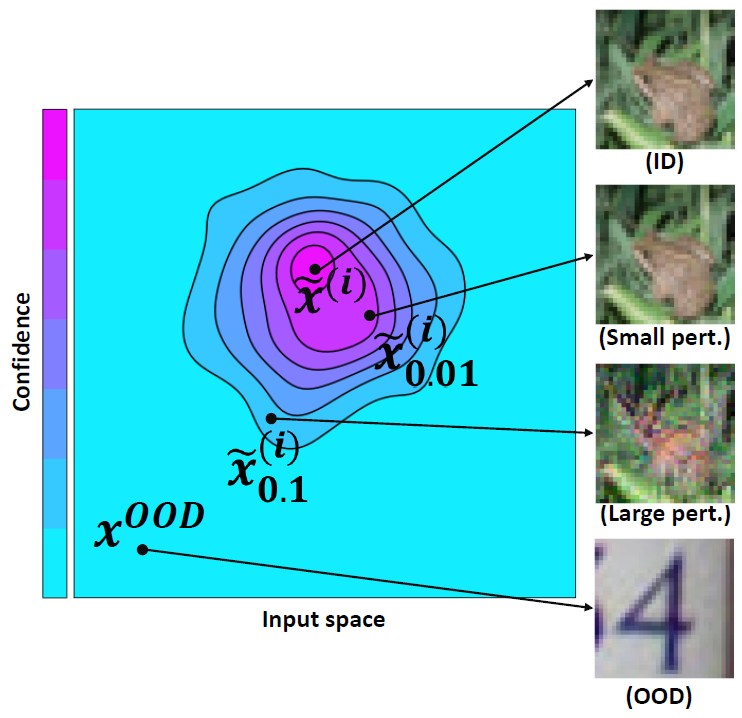
\includegraphics[width=0.36\textwidth]{sections/008_icml2021/eval/uncertainty_diagram.png}
\caption{Visualization of the desired uncertainty estimates. 
}
\label{fig:uncertainty_attack_diagram}
\end{figure}
%
DBU models have the advantage that they provide both, aleatoric uncertainty estimates resulting from irreducible uncertainty (e.g. class overlap or noise) and epistemic uncertainty estimates resulting from the lack of knowledge about unseen data (e.g. an unknown object is presented to the model). Both uncertainty types can be quantified from Dirichlet distributions using different uncertainty measures such as differential entropy, mutual information, or pseudo-counts. These uncertainty measures show outstanding performance in, e.g., the detection of OOD samples and thus are superior to softmax based confidence \citep{malini2018, reverse-kl, charpentier2020}.

Neural networks from the families outlined above are expected to \emph{know what they don't know}, i.e. they are supposed to notice when they are unsure about a prediction. 
This raises questions with regards to adversarial examples: should uncertainty estimation methods \emph{detect} these corrupted samples by indicating a high uncertainty on them and abstain from making a prediction? Or should uncertainty estimation be \emph{robust} to adversarial examples and assign the correct label even under perturbations? We argue that being robust to adversarial perturbations is the best option (see \cref{fig:uncertainty_attack_diagram}) for two reasons. First, in image classification a human is usually not able to observe any difference between an adversarial example and an unperturbed image. Second, the size of the perturbation corresponding to a good adversarial example is typically small w.r.t.\ the $L_p$-norm and thus assumed to be semantically meaningless. 
Importantly, robustness should not only be required for the class predictions, but also for the uncertainty estimates. This means that DBU models should be able to distinguish robustly between ID and OOD data even if those are perturbed. 
%Importantly, one should require robustness not only for the class predictions, but also for the uncertainty estimation. This means that DBU models should be able to distinguish robustly between ID and OOD data even if those are perturbed. 

In this chapter, we focus on DBU models and analyze their robustness capacity w.r.t. class predictions as well as uncertainty predictions. In doing so, we go beyond simple softmax output confidence by investigating advanced uncertainty measures such as differential entropy.
Specifically, we study the following questions: 
%
\begin{enumerate}
    \item \emph{Is low uncertainty a reliable indicator of correct predictions?}
    \item \emph{Can we use uncertainty estimates to detect label attacks on the class prediction?}
    \item \emph{Are uncertainty estimates such as differential entropy a robust feature for OOD detection?}
\end{enumerate}

In addressing these questions we place particular focus on adversarial perturbations of the input to evaluate the \emph{worst case} performance of the models on increasing complex data sets and attacks.
%
We evaluate robustness of DBU models w.r.t. to these three questions by comparing their performance on unperturbed and perturbed inputs. Perturbed inputs are obtained by computing \emph{label attacks} and \emph{uncertainty attacks}, which are a new type of attacks we propose.  While label attacks aim at changing the class prediction, uncertainty attacks aim at changing the uncertainty estimate such that ID data is marked as OOD data and vice versa.
%
In total, we performed more than $138,800$ attack settings to explore the robustness landscape of DBU models. Those settings cover different data sets, attack types, attack losses, attack radii, DBU model types and initialisation seeds.
%
Finally, we propose and evaluate median smoothing and adversarial training based on label attacks and uncertainty attacks to make DBU models more robust. Our median smoothing approach provides certificates on epistemic uncertainty measures such as differential entropy and allows to certify uncertainty estimation.  The code and further supplementary material is available online (\url{www.daml.in.tum.de/dbu-robustness}).





\section{Related work}
\label{sec:related_work}

% add papers not related to this work
The existence of adversarial examples is a problematic property of neural networks \citep{szegedy2014, goodfellow2014}. Previous works have study this phenomena by proposing adversarial attacks \citep{carlini2016, brendel2018,DBLP:conf/kdd/ZugnerAG18}, defenses \citep{cisse2017, gu2015} and verification techniques  \citep{wong2017, singh2019krelu, cohen2019, DBLP:conf/icml/BojchevskiKG20, kopetzki2021}. This includes the study of different settings such as i.i.d. inputs, sequential inputs and graphs \citep{zheng2016, DBLP:conf/nips/BojchevskiG19, cheng2020, schuchardt2021}.

% related work
In the context of uncertainty estimation, robustness of the class prediction has been studied in previous works for Bayesian Neural Networks \citep{blundell2015, osawa2019, wesley2019}, drop out \citep{drop_out} or ensembles \citep{ensemble_simple} focusing on data set shifts \cite{snoek2019} or adversarial attacks \cite{robustness_bnn, cardelli2019, wicker2020}. Despite their efficient and high quality uncertainty estimates, the robustness of DBU models has not been investigated in detail yet --- indeed only for one single DBU model, \citep{malinin2019} has briefly performed attacks aiming to change the label. 
In contrast, our work focuses on a large variety of DBU models and analyzes two robustness properties: robustness of the class prediction w.r.t. adversarial perturbations and robustness of uncertainty estimation w.r.t.\ our newly proposed attacks against uncertainty measures. 


This so called \emph{uncertainty attack} directly targets uncertainty estimation and are different from traditional \emph{label attacks}, which target the class prediction \citep{madry2018, raphael2020}. They allow us to jointly evaluate robustness of the class prediction and robustness of uncertainty estimation. This goes beyond previous attack defenses that were either focused on evaluating \emph{robustness w.r.t.\ class predictions} \citep{carlini2016, clever_robustness} or detecting attacks against the class prediction \citep{bypassing_attack_detection}. 


Different models have been proposed to account for uncertainty while being robust.  \citep{smith2018} and \citep{simple_ood_adv_detection} have tried to improve label attack detection based on uncertainty using drop-out or density estimation. In addition to improving label attack detection for large unseen perturbations, \citep{stutz2020} aimed at improving robustness w.r.t. class label predictions on small input perturbations. They used adversarial training and soft labels for adversarial samples further from the original input. \citep{qin2020} suggested a similar adversarial training procedure, that softens labels depending on the input robustness. These previous works consider the aleatoric uncertainty that is contained in the predicted categorical probabilities, but in contrast to DBU models they are not capable of taking epistemic uncertainty into account. 



Recently, four studies tried to obtain certificates on aleatoric uncertainty estimates. \citep{single_model_quantile} and \citep{confidence_certificate_rs} compute confidence intervals and certificates on softmax predictions. \citep{bitterwolf2020} uses interval bound propagation to compute bounds on softmax predictions within the $L_{\infty}$-ball around an OOD sample using ReLU networks. \citep{meinke2020} focuses on obtaining certifiably low confidence for OOD data. These four studies estimate confidence based on softmax predictions, which accounts for aleatoric uncertainty only. In this paper, we provide certificates which apply for all uncertainty measures. In particular, we use our certificates on epistemic uncertainty measures such as differential entropy which are well suited for OOD detection.



% List of Papers on Robustness (group website)
%
%Anna-Kathrin Kopetzki, Stephan Günnemann
%Reachable sets of classifiers and regression models: (non-)robustness analysis and robust training
%Machine Learning Journal, 2021 --> cited
%
%Jan Schuchardt, Aleksandar Bojchevski, Johannes Klicpera, Stephan Günnemann
%Collective Robustness Certificates: Exploiting Interdependence in Graph Neural Networks
%International Conference on Learning Representations (ICLR), 2021
%
%Simon Geisler, Daniel Zügner, Stephan Günnemann
%Reliable Graph Neural Networks via Robust Aggregation
%Neural Information Processing Systems (NeurIPS), 2020
%
%Aleksandar Bojchevski, Johannes Klicpera, Stephan Günnemann
%Efficient Robustness Certificates for Discrete Data: Sparsity-Aware Randomized Smoothing for Graphs, Images and More
%International Conference on Machine Learning (ICML), 2020
%
%Daniel Zügner, Stephan Günnemann
%Certifiable Robustness of Graph Convolutional Networks under Structure Perturbations
%ACM SIGKDD Conference on Knowledge Discovery and Data Mining (KDD), 2020
%
%Daniel Zügner, Oliver Borchert, Amir Akbarnejad, Stephan Günnemann
%Adversarial Attacks on Graph Neural Networks: Perturbations and their Patterns
%ACM Transactions on Knowledge Discovery from Data, 2020
%
%Aleksandar Bojchevski, Stephan Günnemann
%Certifiable Robustness to Graph Perturbations
%Neural Information Processing Systems (NeurIPS), 2019
%
%Daniel Zügner, Stephan Günnemann
%Certifiable Robustness and Robust Training for Graph Convolutional Networks
%ACM SIGKDD Conference on Knowledge Discovery and Data Mining (KDD), 2019
%
%Aleksandar Bojchevski, Stephan Günnemann
%Adversarial Attacks on Node Embeddings via Graph Poisoning
%International Conference on Machine Learning (ICML), 2019
%
%Daniel Zügner, Stephan Günnemann
%Adversarial Attacks on Graph Neural Networks via Meta Learning
%International Conference on Learning Representations (ICLR), 2019
%
%Daniel Zügner, Amir Akbarnejad, Stephan Günnemann
%Adversarial Attacks on Neural Networks for Graph Data (Extended Abstract)
%International Joint Conference on Artificial Intelligence (IJCAI), 2019
%(Invited contribution to the IJCAI Sister Conference Best Paper Track)
%
%Daniel Zügner, Amir Akbarnejad, Stephan Günnemann
%Adversarial Attacks on Neural Networks for Graph Data 
%(Best Research Paper Award)
%ACM SIGKDD Conference on Knowledge Discovery and Data Mining (KDD), 2018
%
%
%Richard Leibrandt, Stephan Günnemann
%Making Kernel Density Estimation Robust towards Missing Values in Highly Incomplete Multivariate Data without Imputation
%SIAM International Conference on Data Mining (SDM), 2018 
%
%Aleksandar Bojchevski, Stephan Günnemann
%Bayesian Robust Attributed Graph Clustering: Joint Learning of Partial Anomalies and Group Structure
%AAAI Conference on Artificial Intelligence, pp. 2738-2745, 2018
%
%Aleksandar Bojchevski, Yves Matkovic, Stephan Günnemann
%Robust Spectral Clustering for Noisy Data: Modeling Sparse Corruptions Improves Latent Embeddings
%ACM SIGKDD Conference on Knowledge Discovery and Data Mining (KDD), pp. 737-746, 2017


\section{Dirichlet-based uncertainty models}
\label{sec:dirichlet_models}
%
Standard (softmax) neural networks predict the parameters of a categorical distribution \smash{$\vp\dataix = [p\dataix_1, \ldots, p\dataix_\nclass]$} for a given input \smash{$\x\dataix \in \mathbb{R}^{d}$}, where $\nclass$ is the number of classes. 
Given the parameters of a categorical distribution, the \emph{ aleatoric uncertainty} can be evaluated. The aleatoric uncertainty is the uncertainty on the class label prediction \smash{$y\dataix \in \{1, \ldots, \nclass\}$}. For example if we predict the outcome of an unbiased coin flip, the model is expected to have high aleatoric uncertainty and predict $p(\text{head})=0.5$.

\begin{table*}[ht]
	\centering
	\caption{Summary of DBU models. Further details on the loss functions are provided in the appendix.}
	\label{tab:dirichlet_models}
	\resizebox{.9 \textwidth}{!}{%
		\begin{tabular}{lllllll}
			\toprule
			{} &  \textbf{$\alpha\dataix$-parametrization} & \textbf{Loss} & \textbf{OOD training data} & \textbf{Ensemble training} & \textbf{Density estimation}\\
			\midrule
			\textbf{\PostNet} & $f_{\theta}(\x\dataix) = \mathbf{1} + \bm{\alpha}\dataix$ & Bayesian loss & No & No & Yes \\
			\textbf{\PriorNet} & $f_{\theta}(\x\dataix) = \bm{\alpha}\dataix$ & Reverse KL & Yes &  No & No \\
			\textbf{\DDNet} & $f_{\theta}(\x\dataix) = \bm{\alpha}\dataix$ & Dir. Likelihood & No & Yes & No \\
			\textbf{\EvNet} & $f_{\theta}(\x\dataix) =  \mathbf{1} + \bm{\alpha}\dataix$ & Expected MSE & No &  No & No \\
			\bottomrule
		\end{tabular}
	}
	%\vspace{-.5cm}
\end{table*}


In contrast to standard (softmax) neural networks, DBU models predict the parameters of a Dirichlet distribution -- the natural prior of categorical distributions -- given input~$\x \dataix$ (i.e. \smash{$q\dataix = \text{Dir}(\bm{\alpha}\dataix)$} where \smash{$f_{\theta}(\x\dataix) = \bm{\alpha} \dataix \in \mathbb{R}_+^\nclass$}). Hence, the \emph{epistemic distribution} \smash{$q\dataix$} expresses the \emph{epistemic} uncertainty on $\x \dataix$, i.e. the uncertainty on the categorical distribution prediction \smash{$\vp\dataix$}. From the epistemic distribution, follows an estimate of the \emph{aleatoric distribution} of the class label prediction $\text{Cat}(\bar{\vp}\dataix)$ where \smash{$\E_{q\dataix}[\vp\dataix] = \bar{\vp}\dataix$}.
An advantage of DBU models is that one pass through the neural network is sufficient to compute epistemic distribution, aleatoric distribution, and predict the class label:
%
\begin{equation}
\begin{aligned}
    q^{(\idata)}           = \text{Dir}(\bm{\alpha}\dataix), \hspace{5pt}
    \bar{p}_\iclass\dataix  = \frac{\alpha_\iclass\dataix}{\alpha_0\dataix}, \hspace{5pt}
    y^{(\idata)}           = \arg \max_{\iclass} \;[\bar{p}_\iclass\dataix]
\end{aligned}
\end{equation}
%
where $\alpha_0\dataix = \sum^{\nclass}_{\iclass=1} \alpha_\iclass\dataix$. This parametrization allows to compute classic uncertainty measures in closed-form such as the total pseudo-count $m\dataix_{\alpha_0} = \sum_\iclass \alpha\dataix_\iclass$, the differential entropy of the Dirichlet distribution $m\dataix_\text{diffE} = h(\text{Dir}(\bm{\alpha}\dataix))$ or the mutual information $m\dataix_\text{MI} = I(y\dataix, \vp\dataix)$ (App. \ref{subsec:appendix_measurecomp}, \citep{malini2018}). 
Hence, these measure can efficiently be used to assign high uncertainty to unknown data, which makes DBU models specifically suited for detection of OOD samples. 





Several recently proposed models for uncertainty estimations belong to the family of DBU models, such as \PriorNet, \EvNet, \DDNet and \PostNet. These models differ in terms of their parametrization of the Dirichlet distribution, the training, and density estimation. An overview of theses differences is provided in Table \ref{tab:dirichlet_models}. In our study we evaluate all recent versions of these models.


Contrary to the other models, Prior Networks \textbf{(\PriorNet)} \citep{malini2018, malinin2019}  require OOD data for training to ``teach'' the neural network the difference between ID and OOD data. \PriorNet is trained with a loss function consisting of two KL-divergence terms. The fist term is designed to learn Dirichlet parameters for ID data, while the second one is used to learn a flat Dirichlet distribution %($\boldsymbol{\alpha} = \boldsymbol{1}$) 
for OOD data: 
%
\begin{equation}
\begin{aligned}
    L_{\mathrm{\PriorNet}} &= \frac{1}{N} \left[\sum_{\x\dataix \in \text{ID data}}  [\mathrm{KL} [\mathrm{Dir} (\alpha^{\mathrm{ID}}) || q\dataix]]  \right. \\
                           &+ \left.\sum_{\x\dataix \in OOD data} [\mathrm{KL} [\mathrm{Dir} (\alpha^{\mathrm{OOD}}) || q\dataix]]\right] \\
\end{aligned}
\end{equation}
%
where $\alpha^{\mathrm{ID}}$ and $\alpha^{\mathrm{OOD}}$ are hyper-parameters. Usually $\alpha^{\mathrm{ID}}$ is set to $1e^{1}$ for the correct class and $1$ for all other classes, while $\alpha^{\mathrm{OOD}}$ is set to $\mathbf{1}$ for all classes.
%
There a two variants of \PriorNet. The first one is trained based on reverse KL-divergence \citep{malinin2019}, while the second one is trained with KL-divergence \citep{malini2018}. In our experiments, we include the most recent reverse version of \PriorNet, as it shows superior performance \citep{malinin2019}. 

Evidential Networks \textbf{(\EvNet)} \citep{sensoy2018} are trained with a loss that computes the sum of squares between the on-hot encoded true label $\vy*\dataix$ and the predicted categorical $\vp\dataix$ under the Dirichlet distribution:
%
\begin{equation}
\begin{aligned}
    L_{\mathrm{\EvNet}} &= \frac{1}{N} \sum_i \E_{\vp\dataix \sim \text{Dir}(\bm{\alpha}\dataix)}||\vy*\dataix - \vp\dataix||^2 \\
\end{aligned}
\end{equation}

Ensemble Distribution Distillation \textbf{(\DDNet)} \citep{malinin2019ensemble} is trained in two steps. First, an ensemble of $M$ classic neural networks needs to be trained. 
Then, the soft-labels \smash{$\{\vp_{m}\dataix\}_{m=1}^{M}$} provided by the ensemble of networks are distilled into a Dirichlet-based network by fitting them with the maximum likelihood under the Dirichlet distribution: 
\begin{equation}
\begin{aligned}
    L_{\mathrm{\DDNet}} &= - \frac{1}{N}  \sum_i \sum_{m=1}^{M} [\ln q\dataix(\pi^{im})] \\
\end{aligned}
\end{equation}
where $\pi^{im}$ denotes the soft-label of $m$th neural network. 

Posterior Network \textbf{(\PostNet)} \citep{charpentier2020} performs density estimation for ID data with normalizing flows and uses a Bayesian loss formulation: %composed of the Uncertain Cross-Entropy loss \citep{uncertainty_time} and an entropy regularizer inspired by Bayesian theory.
\begin{equation}
\begin{aligned}
    L_{\mathrm{\PostNet}} &= \frac{1}{N} \sum_i \E_{q(p\dataix)}  [\mathrm{CE} (p\dataix, y\dataix)] - H(q\dataix)
\end{aligned}
\end{equation}
where $\mathrm{CE}$ denotes the cross-entropy.
%
All loss functions can be computed in closed-form. For more details please have a look at the original paper on \PriorNet \citep{malini2018}, \PostNet \citep{charpentier2020}, \DDNet \citep{malinin2019} and \EvNet \citep{sensoy2018}.
Note that \EvNet and \PostNet model the Dirichlet parameters as \smash{$f_{\theta}(\x\dataix) = 1 + \bm{\alpha}\dataix$} while \PriorNet, \RevPriorNet and \DDNet compute them as \smash{$f_{\theta}(\x\dataix) = \bm{\alpha}\dataix$}. 









\section{Robustness of Dirichlet-based uncertainty models}
\label{sec:attack_dirichlet_model}

We analyze robustness of DBU models on tasks in connection with uncertainty estimation w.r.t.\ the following four aspects: \emph{accuracy}, \emph{confidence calibration}, \emph{label attack detection} and \emph{OOD detection}. Uncertainty is quantified by differential entropy, mutual information or pseudo counts. 
A formal definition of all uncertainty estimation measures is provided in the appendix (see Section~\ref{subsec:appendix_measurecomp}).  

Robustness of Dirichlet-based uncertainty models is evaluated based on \emph{label attacks} and a newly proposed type of attacks called \emph{uncertainty attacks}. 
While label attacks aim at changing the predicted class, uncertainty attacks aim at changing the uncertainty assigned to a prediction. 
All previous works are based on label attacks and focus on robustness w.r.t. the class prediction. Thus, we are the first to propose attacks targeting uncertainty estimates such as differential entropy and analyze desirable robustness properties of DBU models beyond the class prediction. 
Label attacks and uncertainty attacks both compute a perturbed input $\tilde{\x}\dataix$ close to the original input~$\x\dataix$ i.e. $|| \x\dataix - \tilde{\x}\dataix ||_2 < r$ where $r$ is the attack radius. This perturbed input is obtained by optimizing a loss function $l(\x)$ using Fast Gradient Sign Method (FGSM) or Projected Gradient Descent (PGD). Furthermore, we include a black box attack setting (Noise) which generates 10 noise samples from a Gaussian distribution, which is centered at the original input. From these 10 perturbed samples we choose the one with the greatest effect on the loss function and use it as attack. 
To complement attacks, we compute certificates on uncertainty estimates using median smoothing \cite{median_smoothing}. 


%Reviewer: avoid redundancy within assessment metric paragraphs, explain high level + differences
The following questions we address by our experiments have a common assessment metric and can be treated as binary classification problems: distinguishing between correctly and wrongly classified samples, discriminating between non-attacked input and attacked inputs or differentiating between ID data and OOD data. To quantify the performance of the models on these binary classification problems, we compute the area under the precision recall curve (AUC-PR).

Experiments are performed on two image data sets (MNIST \citep{mnist} and CIFAR10 \citep{cifar10}), which contain bounded inputs and two tabular data sets (Segment \citep{uci_datasets} and Sensorless drive \citep{uci_datasets}), consisting of unbounded inputs. Note that unbounded inputs are challenging since it is impossible to describe the infinitely large OOD distribution. As PriorNet requires OOD training data, we use two further image data sets (FashionMNIST \citep{fashionmnist} and CIFAR100 \citep{cifar10}) for training on MNIST and CIFAR10, respectively. All other models are trained without OOD data. To obtain OOD data for the tabular data sets, we remove classes from the ID data set (class window for the Segment data set and class 9 for Sensorless drive) and use them as the OOD data. Further details on the experimental setup are provided in the appendix (see Section~\ref{subsec:exp_setup}).



 


\subsection{Uncertainty estimation under label attacks}
\label{subsec:label_attacks}
%
Label attacks aim at changing the predicted class. To obtain a perturbed input with a different label, we maximize the cross-entropy loss $\tilde{\x}\dataix \approx \arg\max_{\x} l(\x) = \text{CE}(\vp\dataix, \vy\dataix)$ under the radius constraint. For the sake of completeness we additionally analyze label attacks w.r.t. to their performance of changing the class prediction and the accuracy of the neural network under label attacks constraint by different radii (see Appendix, Table~\ref{tab:acc_label_attack}). As expected and partially shown by previous works, none of the DBU models is robust against label attacks. %, neither on the image data sets nor on the tabular data sets.
However, we note that \PriorNet is slightly more robust than the other DBU models. This might be explained by the use of OOD data during training, which can be seen as some kind of robust training. 
%
From now on, we switch to the core focus of this work and analyze robustness properties of uncertainty estimation. 




\begin{table*}[ht]
	\centering
	\caption{Distinguishing between correctly predicted and wrongly predicted labels based on the differential entropy under PGD label attacks (metric: AUC-PR).}
	%\begin{small}
	\resizebox{0.8\textwidth}{!}{
		\begin{tabular}{@{}rrrrrrrc|crrrrrr@{}}
			\toprule
			& \multicolumn{6}{c}{CIFAR10} & & & \multicolumn{6}{c}{Sensorless} \\
			\cmidrule{2-7}  \cmidrule{10-15}
			Att. Rad. & 0.0 & 0.1 & 0.2 & 0.5 & 1.0 & 2.0 & & & 0.0 & 0.1 & 0.2 & 0.5 & 1.0 & 2.0  \\
			\midrule
			%& \multicolumn{7}{c}{MNIST} & & & \multicolumn{7}{c}{CIFAR10} \\
			\PostNet  &  \bf{98.7} &  88.6 &  56.2 &   7.8 &   1.2 &   0.4 &  & %0.3 & & 
			&  99.7 &   8.3 &   3.9 &  3.6 &  \bf{7.0} &  \bf{9.8} \\%&  \bf{11.3} \\
			\PriorNet &  92.9 &  77.7 &  60.5 &  \bf{37.6} &  \bf{24.9} &  \bf{11.3} &  & %\bf{3.0} & & 
			&  99.8 &  10.5 &   3.2 &  0.7 &  0.2 &  0.2 \\%&   2.2 \\ 
			\DDNet    &  97.6 &  \bf{91.8} &  \bf{78.3} &  18.1 &   0.8 &   0.0 &  &%0.0 & &
			&  99.7 &  11.9 &   1.6 &  0.4 &  0.2 &  0.1 \\%&   0.2 \\ 
			\EvNet    &  97.9 &  85.9 &  57.2 &  10.2 &   4.0 &   2.4 &  &%0.3 & & 
			&  \bf{99.9} &  \bf{22.9} &  \bf{13.0} &  \bf{6.0} &  3.7 &  3.2 \\%&   3.1 \\
			\bottomrule
		\end{tabular}}
	%\end{small}
	\label{tab:conf_label_attack}
\end{table*}







\textbf{Is low uncertainty a reliable indicator of correct predictions?} \\
%
\underline{\emph{Expected behavior:}}  Predictions with low uncertainty are more likely to be correct than high uncertainty predictions. 
\underline{\emph{Assessment metric:}} We distinguish between correctly classified samples (label 0) and wrongly classified ones (label 1) based on the differential entropy scores produced by the DBU models \citep{malini2018}. Correctly classified samples are expected to have low differential entropy, reflecting the model's confidence, and analogously wrongly predicted samples are expected to have higher differential entropy. 
%\dz{State that the metric is AUC-PR?} 
\underline{\emph{Observed behavior:}} Note that the positive and negative class are not balanced, thus, the use of AUC-PR scores \citep{imbalance_apr} are important to enable meaningful measures. While uncertainty estimates are indeed an indicator of correctly classified samples on unperturbed data, none of the models maintains its high performance on perturbed data computed by PGD, FGSM or Noise label attacks (see. Table~\ref{tab:conf_label_attack}, \ref{tab:conf_label_attack_fgsm} and \ref{tab:conf_label_attack_noise_attack}). Thus, using uncertainty estimates as indicator for correctly labeled inputs is not robust to adversarial perturbations. This result is notable, since the used attacks do not target uncertainty. 





\vspace{1em}
\begin{table*}[ht]
	\centering
	\caption{Label Attack-Detection by normally trained DBU models based on differential entropy under PGD label attacks (AUC-PR).}
	%\begin{small}
	\resizebox{0.8\textwidth}{!}{
		\begin{tabular}{@{}rrrrrrc|crrrrr@{}}
			\toprule
			& \multicolumn{5}{c}{CIFAR10} & & & \multicolumn{5}{c}{Sensorless} \\
			\cmidrule{2-6}  \cmidrule{9-13}
			Att. Rad. & 0.1 & 0.2 & 0.5 & 1.0 & 2.0 & & & 0.1 & 0.2 & 0.5 & 1.0 & 2.0 \\
			\midrule
			\PostNet  &  \bf{63.4} &  \bf{66.9} &  42.1 &  32.9 &  31.6 &  &%31.2 & & 
			&  47.7 &  42.3 &  36.9 &  \bf{48.5} &  \bf{85.0} \\%&  \bf{99.0} \\ 
			\PriorNet &  53.3 &  56.0 &  55.6 &  \bf{49.2} &  42.2 & &%  35.4 & & 
			&  38.8 &  33.6 &  31.4 &  33.1 &  40.9 \\%&  53.5 \\ 
			\DDNet    &  55.8 &  60.5 &  \bf{57.3} &  38.7 &  32.3 & &% 31.4 & & 
			&  \bf{53.5} &  42.2 &  35.0 &  32.8 &  32.6 \\%&  33.9 \\ 
			\EvNet    &  48.4 &  46.9 &  46.3 &  46.3 &  \bf{44.5} & &% \bf{42.5} & &
			&  48.2 &  \bf{42.6} &  \bf{38.2} &  36.0 &  37.2 \\%&  41.7 \\
			\bottomrule 			
		\end{tabular}}
	%\end{small}
	\label{tab:label_attack_detect}
\end{table*}








%\vspace{-0.5em}
\textbf{Can uncertainty estimates be used to detect label attacks against the class prediction?}\\
%
\underline{\emph{Expected behavior:}} Adversarial examples are not from the natural data distribution. Therefore, DBU models are expected to detect them as OOD data by assigning them a higher uncertainty. We expect that perturbations computed based on a bigger attack radius~$r$ are easier to detect as their distance from the data distribution is larger. 
\underline{\emph{Assessment metric:}} The goal of attack-detection is to distinguish between unperturbed samples (label 0) and perturbed samples (label 1). Uncertainty on samples is quantified by the differential uncertainty \citep{malini2018}. Unperturbed samples are expected to have low differential entropy, because they are from the same distribution as the training data, while perturbed samples are expected to have a high differential entropy. 
%Further results based on other uncertainty measures are provided in the appendix. 
\underline{\emph{Observed behavior:}} Table~\ref{tab:acc_label_attack} shows that the accuracy of all models decreases significantly under PGD label attacks, but none of the models is able to provide an equivalently increasing attack detection rate (see Table~\ref{tab:label_attack_detect}). Even larger perturbations are hard to detect for DBU models. 

Similar results are obtained when we use mutual information or the precision~$\alpha_0$ to quantify uncertainty (see appendix Table~\ref{tab:conf_label_attack_mi} and~\ref{tab:conf_label_attack_alpha}).
Although PGD label attacks do not explicitly consider uncertainty, they seem to generate adversarial examples with similar uncertainty as the original input. 
Such high-certainty adversarial examples are illustrated in Figure~\ref{fig:attaked_samples_labels}, where certainty is visualized based on the precision~$\alpha_0$, which is supposed to be high for ID data and low for OOD data. While the original input (perturbation size $0.0$) is correctly classified as frog and ID data, there exist adversarial examples that are classified as deer or bird. The certainty ($\alpha_0$-score) on the prediction of these adversarial examples has a similar or even higher value than on the prediction of the original input. Using the differential entropy to distinguish between ID and OOD data results in the same ID/OOD assignment since the differential entropy of the three right-most adversarial examples is similar or even smaller than on the unperturbed input. 







Under the less powerful FGSM and Noise attacks (see Appendix), DBU models achieve mostly higher attack detection rates than under PGD attacks. This suggests that uncertainty estimation is able to detect weak attacks, which is consistent with the observations in \citep{malinin2018_adetect} but fails under stronger PGD attacks. 
%
\begin{figure}[ht]
	\centering
	\resizebox{0.42\textwidth}{!}{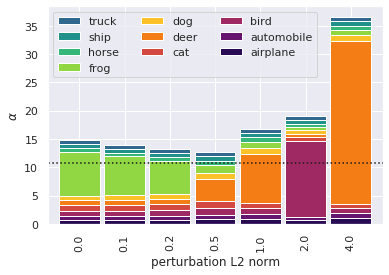
\includegraphics[width=\textwidth]{sections/008_icml2021/eval/ddnet_label_id_cifar10_alphas.png}}%
	\resizebox{0.42\textwidth}{!}{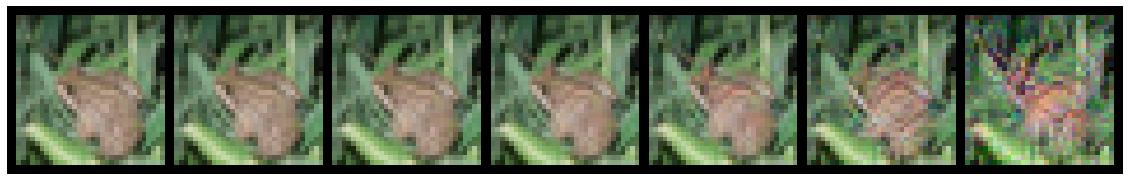
\includegraphics[width=\textwidth]{sections/008_icml2021/eval/ddnet_label_id_cifar10_images.png}}
	\caption{Input and predicted Dirichlet-parameters under label attacks (dotted line: threshold to distinguish ID and OOD data). % based on the precision~$\alpha_0$.
		%-14.2216765174
		%0.0 [-17.875761]
		%0.1 [-17.257824]
		%0.2 [-16.648003]
		%0.5 [-15.014889]
		%1.0 [-17.504786]
		%2.0 [-22.63896]
		%4.0 [-24.941536]
	}
	\label{fig:attaked_samples_labels}
\end{figure}


On tabular data sets, \PostNet shows a better label attack detection rate for large perturbations. This observation might be explained by the fact that the density estimation of the ID samples has been shown to work better for tabular data sets \citep{charpentier2020}. 
%
Overall, none of the DBU models provides a reliable indicator for adversarial inputs that target the class prediction. 





\vspace{.4mm}
\begin{table*}[ht]
	\centering
	\caption{OOD detection based on differential entropy under PGD uncertainty attacks against differential entropy computed on ID data and OOD data (metric: AUC-PR).}
%	\begin{small}
	\resizebox{\textwidth}{!}{
		\begin{tabular}{@{}rrrrrrrc|crrrrrr@{}}
			\toprule
			& \multicolumn{6}{c}{ID-Attack (non-attacked OOD)} &  & &  \multicolumn{6}{c}{OOD-Attack (non-attacked ID)} \\
			\cmidrule{2-7}  \cmidrule{10-15}
			Att. Rad. & 0.0 & 0.1 & 0.2 & 0.5 & 1.0 & 2.0 & & &
			0.0 & 0.1 & 0.2 & 0.5 & 1.0 & 2.0  \\
			\midrule
			& \multicolumn{14}{c}{\textbf{CIFAR10 -- SVHN}} \\
			\PostNet  &  81.8 &  64.3 &  47.2 &  22.4 &  17.6 &  \bf{16.9} &  &%\bf{16.4} & &
			&  81.8 &  60.5 &  40.7 &  23.3 &  21.8 &  19.8 \\%&  18.1 \\ 
			\PriorNet &  54.4 &  40.1 &  30.0 &  17.9 &  15.6 &  15.4 &  &%15.4 & &
			&  54.4 &  40.7 &  30.7 &  19.5 &  16.5 &  15.7 \\%&  15.4 \\
			\DDNet    &  \bf{82.8} &  \bf{71.4} &  \bf{59.2} &  \bf{28.9} &  16.0 &  15.4 & &% 15.4 & &
			&  \bf{82.8} &  \bf{72.0} &  \bf{57.2} &  20.8 &  15.6 &  15.4 \\%&  15.4 \\
			\EvNet    &  80.3 &  62.4 &  45.4 &  21.7 &  \bf{17.9} &  16.5 &  &%15.6 & &
			&  80.3 &  58.2 &  46.5 &  \bf{34.6} &  \bf{28.0} &  \bf{23.9} \\%&  \bf{21.0} \\
			\midrule
			& \multicolumn{14}{c}{\textbf{Sens. -- Sens. class 10, 11}} \\
			\PostNet  &  \bf{74.5} &  \bf{39.8} &  \bf{36.1} &  \bf{36.0} &  \bf{45.9} &  \bf{46.0} & &% \bf{46.0} & &
			&  \bf{74.5} &  \bf{43.3} &  \bf{42.0} &  \bf{32.1} &  \bf{35.1} &  \bf{82.6} \\%&  \bf{99.4} \\
			\PriorNet &  32.3 &  26.6 &  26.5 &  26.5 &  26.6 &  28.3 & &% 38.6 & &
			&  32.3 &  26.7 &  26.6 &  26.6 &  27.0 &  30.4 \\%&  36.8 \\ 
			\DDNet    &  31.7 &  26.8 &  26.6 &  26.5 &  26.6 &  27.1 & &% 30.5 & &
			&  31.7 &  27.1 &  26.7 &  26.7 &  26.8 &  26.9 \\%&  27.3 \\ 
			\EvNet    &  66.5 &  30.5 &  28.2 &  27.1 &  28.1 &  31.8 & &% 37.5 & &
			&  66.5 &  38.7 &  36.1 &  30.2 &  28.2 &  28.8 \\%&  32.2 \\
			\bottomrule
		\end{tabular}}
%	\end{small}
	\label{tab:id_ood_attacks}
\end{table*}









\subsection{Attacking uncertainty estimation}
\label{subsec:uncertainty_attacks}

DBU models are designed to provide sophisticated uncertainty estimates (beyond softmax scores) alongside predictions and use them to detect OOD samples. In this section, we propose and analyze a new attack type that targets these uncertainty estimates. 
DBU models enable us to compute uncertainty measures i.e. differential entropy, mutual information and precision~$\alpha_0$ in closed from (see \citep{malini2018} for a derivation). Uncertainty attacks use this closed form solution as loss function for PGD, FGSM or Noise attacks. 
Since differential entropy is the most widely used metric for ID-OOD-differentiation, we present results based on the differential entropy loss function $\tilde{\x}\dataix \approx \arg\max_{\x} l(\x) = \text{Diff-E}(\text{Dir}(\mathbf{\alpha}\dataix))$: 
%
\begin{equation}
\begin{aligned}
	\text{Diff-E}(\text{Dir}(\mathbf{\alpha}\dataix))  = &\sum_c^K \ln \Gamma (\alpha_c^{(i)}) - \ln \Gamma (\alpha_0^{(i)}) \\
	&- \sum_c^K (\alpha_c^{(i)} -1) \cdot (\Psi (\alpha_c^{(i)}) - \Psi (\alpha_0^{(i)}))
\end{aligned}
\end{equation}
%
where $\alpha_0^{(i)} = \sum_c \alpha_c^{(i)}$. 
Result based on further uncertainty measures, loss functions and more details on attacks are provided in the appendix. 


We analyze the performance of DBU models under uncertainty attacks w.r.t.\ two tasks. First, uncertainty attacks are computed on ID data aiming to indicate it as OOD data, while OOD data is left non-attacked. Second, we attack OOD data aiming to indicate it as ID data, while ID data is not attacked. Hence, uncertainty attacks target at posing ID data as OOD data and vice versa.


\begin{figure}[ht!]
    \centering
        \begin{subfigure}[t]{0.49\columnwidth}
        \centering
        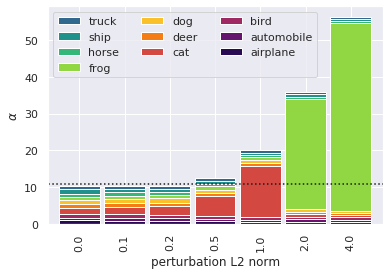
\includegraphics[width=0.99 \textwidth]{sections/008_icml2021/eval/ddnet_unc_ood_cifar10_alphas.png}
    \end{subfigure}%
    \begin{subfigure}[t]{0.49\columnwidth}
        \centering
        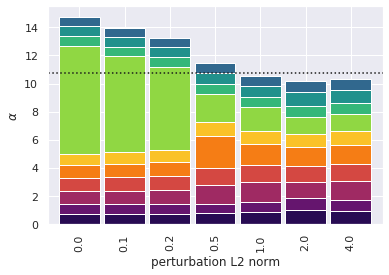
\includegraphics[width=0.99 \textwidth]{sections/008_icml2021/eval/ddnet_unc_id_cifar10_alphas.png}
    \end{subfigure}%


    \begin{subfigure}[t]{0.49 \columnwidth}
        \centering
        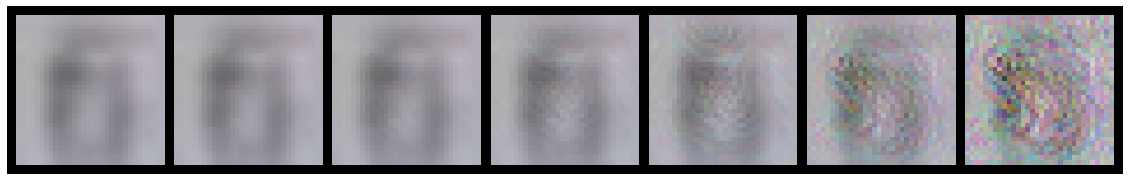
\includegraphics[width=0.99 \textwidth]{sections/008_icml2021/eval/ddnet_unc_ood_cifar10_images.png}
        \caption{OOD uncertainty attack
        %-14.2216765174
        %0.0 [-13.115507]
        %0.1 [-13.353642]
        %0.2 [-13.723262]
        %0.5 [-16.341246]
        %1.0 [-22.298155]
        %2.0 [-28.071136]
        %4.0 [-33.148224]
        }
        \label{fig:attaked_samples_idood_a}
    \end{subfigure}%
        \begin{subfigure}[t]{0.49 \columnwidth}
        \centering
        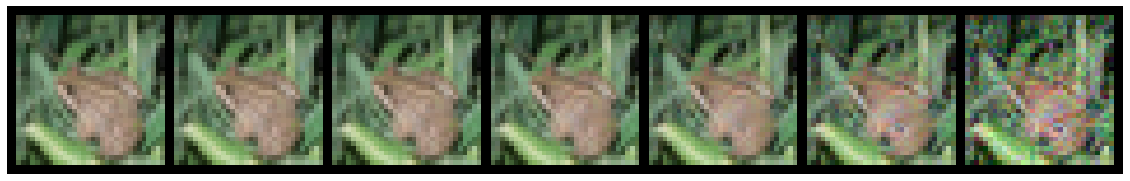
\includegraphics[width=0.99 \textwidth]{sections/008_icml2021/eval/ddnet_unc_id_cifar10_images.png}
        \caption{ID uncertainty attack
        %-14.2216765174
        %0.0 [-17.875761]
        %0.1 [-17.256058]
        %0.2 [-16.65203]
        %0.5 [-14.321844]
        %1.0 [-13.6354265]
        %2.0 [-13.046129]
        %4.0 [-13.1426115]
        }
        \label{fig:attaked_samples_idood_b}
    \end{subfigure}%
    \caption{ID and OOD input with corresponding Dirichlet-parameters under uncertainty attacks (dotted line: threshold to distinguish ID and OOD).}
    \label{fig:attaked_samples_idood}
	%\vspace{-.5cm}
\end{figure}





\textbf{Are uncertainty estimates a robust feature for OOD detection?}\\
%
\underline{\emph{Expected behavior:}} We expect DBU models to be able to distinguish between ID and OOD data by providing reliable uncertainty estimates, even under small perturbations. Thus, we expect uncertainty estimates of DBU models to be robust under attacks. 
%
\underline{\emph{Assessment metric:}} We distinguish between ID data (label 0) and OOD data (label 1) based on the differential entropy as uncertainty scoring function \citep{malini2018}. Differential entropy is expected to be small on ID samples and high on OOD samples. Experiments on further uncertainty measure and results on the AUROC metric are provided in the appendix. 
%
\underline{\emph{Observed behavior:}} OOD samples are perturbed as illustrated in  Figure~\ref{fig:attaked_samples_idood}. Part (a) of the figure illustrates an OOD-samples, that is correctly identified as OOD. Adding adversarial perturbations $\geq 0.5$ changes the Dirichlet parameters such that the resulting images are identified as ID, based on precision or differential entropy as uncertainty measure. Perturbing an ID sample (part (b)) results in images that are marked as OOD samples. 
OOD detection performance of all DBU models rapidly decreases with the size of the perturbation, regardless of whether attacks are computed on ID or OOD data (see Table~\ref{tab:id_ood_attacks}). This performance decrease is also observed with AUROC as metric, attacks based on FGSM, Noise, when we use mutual information or precision~$\alpha_0$ to distinguish between ID samples and OOD samples (see appendix Table~\ref{tab:id_ood_attacks_part2} - \ref{tab:id_ood_attacks_measure_diffE_aupr_noise}). 
Thus, using uncertainty estimation to distinguish between ID and OOD data is not robust. 








\begin{table*}[ht!]
	\centering
	%\begin{tiny}
	\resizebox{\textwidth}{!}{ %0.866
%    \begin{tabular}{lccccccc}
%    \toprule
 %   \textbf{Att. Rad.} & 0.0 &   0.1 &  0.2 &  0.5 &  1.0 &  2.0 \\
 %   \midrule
  %  & \multicolumn{6}{c}{\textbf{Smoothed models}} \\
%    \input{tables_v2/normal-cifar10-in-PGD_L2-crossentropy-confidence}
%    \midrule
%    & \multicolumn{6}{c}{\textbf{Smoothed models + adversarial training using label attacks}} \\
%    \input{tables_v2/adv-cifar10-in-PGD_L2-crossentropy-confidence}
%    \midrule
%    & \multicolumn{6}{c}{\textbf{Smoothed models + adversarial training using uncertainty attacks}} \\
%    \input{tables_v2/unc_adv-cifar10-in-PGD_L2-crossentropy-confidence}
%    \bottomrule
%    \end{tabular}
    \begin{tabular}{clccccccc}
    \toprule
    & \textbf{Att. Rad.} & 0.0 &   0.1 &  0.2 &  0.5 &  1.0 &  2.0 \\
    \midrule
    %& & \multicolumn{6}{c}{\textbf{Smoothed models}} \\
      \multirow{4}{1.2cm}{Smoothed models} & \textbf{PostNet} &  $80.5\cdot\bm{{\color{black}91.5}}\cdot94.5$ &  
  $52.8\cdot\bm{{\color{black}71.6}}\cdot95.2$ &  
  $31.9\cdot\bm{{\color{black}51.0}}\cdot96.8$ &  
  $\phantom{0}5.6\cdot\bm{{\color{blue}11.7}}\cdot100.0$ &  
  $\phantom{0}0.3\cdot\bm{{\color{black}\phantom{0}0.6}}\cdot100.0$ &  
  $\phantom{0}0.0\cdot\bm{{\color{black}\phantom{0}0.0}}\cdot100.0$ \\
 & \textbf{PriorNet} &  
 $81.9\cdot\bm{{\color{black}86.8}}\cdot88.0$ &     
 $69.6\cdot\bm{{\color{blue}78.0}}\cdot90.1$ &     
 $50.9\cdot\bm{{\color{blue}65.8}}\cdot89.4$ & 
 $36.5\cdot\bm{{\color{blue}59.9}}\cdot\phantom{0}97.0$ &   
 $24.3\cdot\bm{{\color{blue}39.3}}\cdot100.0$ &    
 $\phantom{0}9.2\cdot\bm{{\color{blue}17.9}}\cdot100.0$ \\
  &   \textbf{DDNet} &  
  $65.9\cdot\bm{{\color{black}81.2}}\cdot83.0$ &  
  $55.8\cdot\bm{{\color{black}70.5}}\cdot87.2$ &  
  $37.8\cdot\bm{{\color{black}56.8}}\cdot88.1$ &  
  $10.1\cdot\bm{{\color{blue}21.9}}\cdot\phantom{0}94.3$ &      
  $\phantom{0}0.9\cdot\phantom{0}\bm{{\color{blue}1.6}}\cdot\phantom{0}99.6$ &                   
  $\phantom{0}0.0\cdot\phantom{0}\bm{0.0}\cdot100.0$ \\
  &   \textbf{EvNet} &  
  $76.3\cdot\bm{{\color{black}90.2}}\cdot91.7$ &  
  $54.7\cdot\bm{{\color{black}74.3}}\cdot95.7$ &  
  $31.6\cdot\bm{{\color{black}51.5}}\cdot94.5$ &   
  $\phantom{0}5.8\cdot\bm{{\color{blue}11.9}}\cdot\phantom{0}86.9$ &     
  $\phantom{0}1.9\cdot\bm{{\color{blue}\phantom{0}7.0}}\cdot100.0$ &     
  $\phantom{0}1.1\cdot\bm{{\color{blue}\phantom{0}4.0}}\cdot100.0$ \\

    \midrule
    %& & \multicolumn{6}{c}{\textbf{Smoothed models + adversarial training using label attacks}} \\
      \multirow{4}{1.2cm}{Smoothed + adv. w. label attacks} &  
  \textbf{PostNet} &  - &  
  $52.1\cdot\bm{{\color{black}71.8}}\cdot95.6$ &  
  $31.2\cdot\bm{{\color{black}47.9}}\cdot96.1$ &  
  $\phantom{0}7.8\cdot\bm{{\color{blue}14.7}}\cdot\phantom{0}98.6$ &    
  $\phantom{0}1.8\cdot\phantom{0}\bm{{\color{blue}4.4}}\cdot100.0$ &  
  $\phantom{0}0.3\cdot\phantom{0}\bm{{\color{black}0.5}}\cdot100.0$ \\
 & \textbf{PriorNet} &  - &  
 $57.6\cdot\bm{{\color{black}71.7}}\cdot88.9$ &     
 $46.1\cdot\bm{{\color{blue}64.5}}\cdot90.1$ &  
 $38.1\cdot\bm{{\color{blue}59.3}}\cdot\phantom{0}99.5$ &  
 $32.3\cdot\bm{{\color{blue}51.7}}\cdot100.0$ &    
 $22.1\cdot\bm{{\color{blue}41.6}}\cdot\phantom{0}97.4$ \\
   & \textbf{DDNet} &  - &  
   $58.6\cdot\bm{{\color{black}78.4}}\cdot92.2$ &  
   $49.4\cdot\bm{{\color{black}66.0}}\cdot90.5$ &  
   $12.0\cdot\bm{{\color{blue}21.4}}\cdot\phantom{0}98.1$ &     
   $\phantom{0}0.8\cdot\phantom{0}\bm{{\color{blue}1.0}}\cdot\phantom{0}96.6$ &                   
   $\phantom{0}0.0\cdot\phantom{0}\bm{0.0}\cdot100.0$ \\
    & \textbf{EvNet} &  - &  
    $24.3\cdot\bm{{\color{black}34.2}}\cdot51.8$ &  
    $32.6\cdot\bm{{\color{black}49.5}}\cdot95.5$ &  
    $\phantom{0}5.9\cdot\bm{{\color{blue}13.0}}\cdot100.0$ &  
    $\phantom{0}2.6\cdot\phantom{0}\bm{{\color{black}5.2}}\cdot\phantom{0}99.9$ &     
    $\phantom{0}2.9\cdot\phantom{0}\bm{{\color{blue}5.9}}\cdot100.0$ \\

    \midrule
    %& & \multicolumn{6}{c}{\textbf{Smoothed models + adversarial training using uncertainty attacks}} \\
    \multirow{4}{1.3cm}{Smoothed + adv. uncert. attacks} &   
\textbf{PostNet} &  - &  
$52.8\cdot\bm{{\color{black}74.2}}\cdot94.6$ &  
$33.0\cdot\bm{{\color{black}49.4}}\cdot87.5$ &   
$\phantom{0}7.7\cdot\bm{{\color{blue}14.2}}\cdot\phantom{0}99.0$ &  
$\phantom{0}0.6\cdot\phantom{0}\bm{{\color{black}1.2}}\cdot100.0$ &    
$\phantom{0}0.7\cdot\phantom{0}\bm{{\color{blue}1.1}}\cdot100.0$ \\
 & \textbf{PriorNet} &  - &  
 $50.6\cdot\bm{{\color{black}68.1}}\cdot88.6$ &     
 $44.4\cdot\bm{{\color{blue}66.1}}\cdot96.0$ &  
 $35.1\cdot\bm{{\color{blue}57.4}}\cdot\phantom{0}98.4$ &   
 $18.4\cdot\bm{{\color{blue}32.2}}\cdot100.0$ &  
 $15.2\cdot\bm{{\color{blue}29.3}}\cdot100.0$ \\
   & \textbf{DDNet} &  - &  
   $68.8\cdot\bm{{\color{black}84.4}}\cdot93.2$ &  
   $45.1\cdot\bm{{\color{black}60.8}}\cdot86.8$ &  
   $12.3\cdot\bm{{\color{blue}22.0}}\cdot\phantom{0}91.0$ &      
   $\phantom{0}0.8\cdot\phantom{0}\bm{{\color{blue}1.7}}\cdot\phantom{0}87.0$ &                  
   $\phantom{0}0.0\cdot\phantom{0}\bm{0.0}\cdot100.0$ \\
&    \textbf{EvNet} &  - &  
$54.2\cdot\bm{{\color{black}73.7}}\cdot96.1$ &  
$30.5\cdot\bm{{\color{black}50.0}}\cdot99.5$ &  
$\phantom{0}7.1\cdot\bm{{\color{blue}13.9}}\cdot100.0$ &      
$\phantom{0}3.7\cdot\phantom{0}\bm{{\color{blue}8.7}}\cdot\phantom{0}75.2$ &    
$\phantom{0}3.3\cdot\phantom{0}\bm{{\color{blue}5.8}}\cdot100.0$ \\

    \bottomrule
    \end{tabular}}
	%\end{tiny}
	\caption{Distinguishing between correctly and wrongly predicted labels based on differential entropy under PGD label attacks. Smoothed DBU models on CIFAR10. Column format: guaranteed lowest performance $\cdot$ empirical performance $\cdot$ guaranteed highest performance (blue: normally/adversarially trained smooth classifier is more robust than the base model).}
	\label{tab:cifar10_smooth_confidence_2}
\end{table*}

\begin{table*}[ht!]
	\centering
	%\begin{tiny}
	\resizebox{\textwidth}{!}{
		\begin{tabular}{clcccccc}
			\toprule
			& \textbf{Att. Rad.} &   0.1 &  0.2 &  0.5 &  1.0 &  2.0 \\
			\midrule
			%& \multicolumn{6}{c}{\textbf{Smoothed models}} \\
			  \multirow{4}{1.2cm}{Smoothed models}  & \textbf{PostNet} &  %$41.3\cdot\bm{{\color{blue}50.1}}\cdot61.7$ & 
  $33.1\cdot\bm{{\color{black}50.4}}\cdot89.9$ &  
  $31.0\cdot\bm{{\color{black}50.2}}\cdot96.9$ &    
  $30.7\cdot\bm{{\color{blue}50.2}}\cdot100.0$ &    
  $30.7\cdot\bm{{\color{blue}50.0}}\cdot100.0$ &  
  $30.7\cdot\bm{{\color{blue}50.2}}\cdot100.0$ \\
 & \textbf{PriorNet} &  
 %$47.4\cdot\bm{{\color{blue}50.1}}\cdot53.0$ & 
 $35.9\cdot\bm{{\color{black}50.6}}\cdot74.5$ &  
 $33.0\cdot\bm{{\color{black}50.3}}\cdot82.8$ &  
 $31.2\cdot\bm{{\color{black}50.0}}\cdot\phantom{0}95.7$ &  
 $30.7\cdot\bm{{\color{black}50.4}}\cdot\phantom{0}99.9$ &  
 $30.7\cdot\bm{{\color{blue}50.4}}\cdot100.0$ \\
   & \textbf{DDNet} &  
   %$47.3\cdot\bm{{\color{blue}50.1}}\cdot53.3$ & 
   $36.3\cdot\bm{{\color{black}50.3}}\cdot76.4$ &  
   $32.8\cdot\bm{{\color{black}49.9}}\cdot84.6$ &  
   $30.8\cdot\bm{{\color{black}50.1}}\cdot\phantom{0}98.0$ &    
   $30.7\cdot\bm{{\color{blue}50.2}}\cdot100.0$ &  
   $30.7\cdot\bm{{\color{blue}50.2}}\cdot100.0$ \\
&    \textbf{EvNet} &  
%$46.0\cdot\bm{{\color{blue}50.1}}\cdot55.6$ & 
$32.9\cdot\bm{{\color{black}50.4}}\cdot89.8$ &  
$31.4\cdot\bm{{\color{black}50.1}}\cdot94.0$ &     
$30.8\cdot\bm{{\color{blue}50.0}}\cdot\phantom{0}98.0$ &    
$30.7\cdot\bm{{\color{blue}50.3}}\cdot100.0$ &  
$30.7\cdot\bm{{\color{blue}49.6}}\cdot100.0$ \\

			\midrule
			%& \multicolumn{6}{c}{\textbf{Smoothed models + adversarial training using label attacks}} \\
			\multirow{4}{1.3cm}{Smoothed + adv. label attacks}  & 
\textbf{PostNet} &   
$32.7\cdot\bm{{\color{black}50.1}}\cdot90.4$ &  
$31.1\cdot\bm{{\color{black}50.2}}\cdot96.5$ &     
$30.7\cdot\bm{{\color{blue}50.2}}\cdot\phantom{0}99.7$ &     
$30.7\cdot\bm{{\color{blue}50.3}}\cdot100.0$ &  
$30.7\cdot\bm{{\color{blue}50.2}}\cdot100.0$ \\
 & \textbf{PriorNet} & % - &  
 $35.2\cdot\bm{{\color{black}51.8}}\cdot78.6$ &  
 $32.8\cdot\bm{{\color{black}51.1}}\cdot84.4$ &  
 $30.8\cdot\bm{{\color{black}50.2}}\cdot\phantom{0}98.7$ &  
 $30.7\cdot\bm{{\color{black}50.5}}\cdot100.0$ &   
 $30.8\cdot\bm{{\color{blue}50.1}}\cdot\phantom{0}98.2$ \\
   & \textbf{DDNet} &  %- & 
   $35.5\cdot\bm{{\color{black}50.6}}\cdot79.2$ &  
   $33.4\cdot\bm{{\color{black}50.3}}\cdot84.1$ &  
   $30.8\cdot\bm{{\color{black}50.1}}\cdot\phantom{0}99.2$ &     
   $30.7\cdot\bm{{\color{blue}50.0}}\cdot100.0$ & 
   $30.7\cdot\bm{{\color{blue}50.5}}\cdot100.0$ \\
&    \textbf{EvNet} &  %- & 
$40.3\cdot\bm{{\color{black}50.4}}\cdot66.8$ &  
$31.4\cdot\bm{{\color{black}50.3}}\cdot95.8$ &    
$30.7\cdot\bm{{\color{blue}50.3}}\cdot100.0$ &     
$30.7\cdot\bm{{\color{blue}50.1}}\cdot100.0$ &  
$30.7\cdot\bm{{\color{blue}50.0}}\cdot100.0$ \\
			\midrule
			%& \multicolumn{6}{c}{\textbf{Smoothed models + adversarial training using uncertainty attacks}} \\
			\multirow{4}{1.3cm}{Smoothed + adv. uncert. attacks} & 
\textbf{PostNet} &  %- &  
$33.3\cdot\bm{{\color{black}50.6}}\cdot88.7$ &  
$32.5\cdot\bm{{\color{black}50.1}}\cdot87.9$ &     
$30.7\cdot\bm{{\color{blue}49.9}}\cdot\phantom{0}99.8$ &     
$30.7\cdot\bm{{\color{blue}50.1}}\cdot100.0$ &  
$30.7\cdot\bm{{\color{blue}50.0}}\cdot100.0$ \\
& \textbf{PriorNet} &  %- & 
$34.5\cdot\bm{{\color{black}51.0}}\cdot80.1$ &  
$31.4\cdot\bm{{\color{black}50.6}}\cdot92.8$ &  
$30.9\cdot\bm{{\color{black}50.0}}\cdot\phantom{0}97.7$ &  
$30.7\cdot\bm{{\color{black}50.1}}\cdot100.0$ &  
$30.7\cdot\bm{{\color{blue}50.0}}\cdot100.0$ \\
 &   \textbf{DDNet} &  %- & 
 $37.4\cdot\bm{{\color{black}50.8}}\cdot74.5$ &  
 $33.4\cdot\bm{{\color{black}50.2}}\cdot83.0$ &  
 $30.9\cdot\bm{{\color{black}50.1}}\cdot\phantom{0}96.8$ &      
 $30.8\cdot\bm{{\color{blue}49.9}}\cdot\phantom{0}98.1$ &  
 $30.7\cdot\bm{{\color{blue}49.9}}\cdot100.0$ \\
  &  \textbf{EvNet} &  %- & 
  $32.8\cdot\bm{{\color{black}50.1}}\cdot92.0$ &  
  $30.8\cdot\bm{{\color{black}50.0}}\cdot99.6$ &    
  $30.7\cdot\bm{{\color{blue}50.1}}\cdot100.0$ &      
  $31.2\cdot\bm{{\color{blue}50.2}}\cdot\phantom{0}96.1$ &  
  $31.0\cdot\bm{{\color{blue}50.0}}\cdot100.0$ \\

			\bottomrule
		\end{tabular}}
	%\end{tiny}
	\caption{Attack detection (PGD label attacks) based on differential entropy. Smoothed DBU models on CIFAR10. Column format: guaranteed lowest performance $\cdot$ empirical performance $\cdot$ guaranteed highest performance (blue: normally/adversarially trained smooth classifier is more robust than the base model).}
	\label{tab:cifar10_smooth_attackdetection_2}
\end{table*}





\begin{table*}[ht!]
	\centering
	%\begin{tiny}
	\resizebox{\textwidth}{!}{
		\begin{tabular}{clccccccc}
			\toprule
			& \textbf{Att. Rad.} & 0.0 &   0.1 &  0.2 &  0.5 &  1.0 &  2.0 \\
			\midrule
			& & \multicolumn{6}{c}{\textbf{ID-Attack}} \\
			  \multirow{4}{1.6cm}{Smoothed models} &  
  \textbf{PostNet} &     
  $72.1\cdot\bm{{\color{blue}82.7}}\cdot88.0$ &  
  $35.0\cdot\bm{{\color{black}56.6}}\cdot97.4$ &     
  $31.9\cdot\bm{{\color{blue}65.6}}\cdot99.8$ &  
  $30.7\cdot\bm{{\color{blue}50.6}}\cdot100.0$ &  
  $30.7\cdot\bm{{\color{blue}46.9}}\cdot100.0$ &  
  $30.7\cdot\bm{{\color{blue}51.6}}\cdot100.0$ \\
& \textbf{PriorNet} &  
$50.2\cdot\bm{{\color{black}53.1}}\cdot55.9$ &     
$33.5\cdot\bm{{\color{blue}43.3}}\cdot65.3$ &     
$31.3\cdot\bm{{\color{blue}39.7}}\cdot69.1$ &   
$31.3\cdot\bm{{\color{blue}48.3}}\cdot\phantom{0}98.2$ &   
$30.7\cdot\bm{{\color{blue}44.4}}\cdot\phantom{0}99.9$ &  
$30.7\cdot\bm{{\color{blue}45.4}}\cdot100.0$ \\
 &   \textbf{DDNet} &  
 $72.0\cdot\bm{{\color{black}75.8}}\cdot79.8$ &  
 $35.6\cdot\bm{{\color{black}46.2}}\cdot69.8$ &  
 $32.9\cdot\bm{{\color{black}50.3}}\cdot87.1$ &   
 $31.1\cdot\bm{{\color{blue}58.7}}\cdot\phantom{0}98.6$ & 
 $30.7\cdot\bm{{\color{blue}59.3}}\cdot100.0$ &  
 $30.7\cdot\bm{{\color{blue}44.5}}\cdot100.0$ \\
  &  \textbf{EvNet} &     
  $79.5\cdot\bm{{\color{blue}87.1}}\cdot92.8$ &  
  $34.1\cdot\bm{{\color{black}58.6}}\cdot95.1$ &     
  $32.5\cdot\bm{{\color{blue}61.2}}\cdot96.9$ &   
  $31.7\cdot\bm{{\color{blue}60.6}}\cdot\phantom{0}98.7$ &  
  $30.7\cdot\bm{{\color{blue}62.4}}\cdot100.0$ &  
  $30.7\cdot\bm{{\color{blue}57.3}}\cdot100.0$ \\

			\midrule
			%& & \multicolumn{6}{c}{\textbf{ID-Attack}} \\
			\multirow{4}{1.3cm}{Smoothed + adv.\ w. label attacks} &  
\textbf{PostNet} &  - & 
$35.0\cdot\bm{{\color{black}58.5}}\cdot97.7$ &  
$31.2\cdot\bm{{\color{black}46.6}}\cdot97.4$ &   
$30.8\cdot\bm{{\color{blue}57.7}}\cdot\phantom{0}99.7$ &  
$30.7\cdot\bm{{\color{blue}49.8}}\cdot100.0$ &  
$30.7\cdot\bm{{\color{blue}50.9}}\cdot100.0$ \\
& \textbf{PriorNet} &  - &  
$31.5\cdot\bm{{\color{black}36.7}}\cdot57.2$ &     
$33.1\cdot\bm{{\color{blue}51.8}}\cdot84.8$ &   
$30.7\cdot\bm{{\color{blue}57.7}}\cdot\phantom{0}98.7$ &   
$30.7\cdot\bm{{\color{blue}40.0}}\cdot\phantom{0}99.9$ &   
$30.9\cdot\bm{{\color{blue}53.6}}\cdot\phantom{0}96.7$ \\
 &   \textbf{DDNet} &  - &  
 $36.2\cdot\bm{{\color{black}50.0}}\cdot78.6$ &  
 $32.1\cdot\bm{{\color{black}41.3}}\cdot70.2$ &  
 $30.8\cdot\bm{{\color{blue}56.4}}\cdot100.0$ &  
 $30.7\cdot\bm{{\color{blue}49.4}}\cdot100.0$ &  
 $30.7\cdot\bm{{\color{blue}54.8}}\cdot100.0$ \\
  &  \textbf{EvNet} &  - &  
  $46.8\cdot\bm{{\color{black}61.0}}\cdot79.7$ &     
  $32.3\cdot\bm{{\color{blue}58.9}}\cdot99.1$ &  
  $30.7\cdot\bm{{\color{blue}45.0}}\cdot100.0$ &  
  $30.7\cdot\bm{{\color{blue}63.3}}\cdot100.0$ &  
  $30.8\cdot\bm{{\color{blue}38.1}}\cdot100.0$ \\

			\midrule
			%& & \multicolumn{6}{c}{\textbf{ID-Attack}} \\
			\multirow{4}{1.3cm}{Smoothed + adv. uncert. attacks} &  
\textbf{PostNet} &  - &  
$35.2\cdot\bm{{\color{black}55.9}}\cdot96.0$ &     
$34.5\cdot\bm{{\color{blue}59.2}}\cdot94.9$ &  
$30.7\cdot\bm{{\color{blue}47.0}}\cdot100.0$ &  
$30.7\cdot\bm{{\color{blue}58.2}}\cdot100.0$ &  
$30.7\cdot\bm{{\color{blue}42.9}}\cdot100.0$ \\
 & \textbf{PriorNet} &  - &  
 $31.8\cdot\bm{{\color{black}38.9}}\cdot64.1$ &     
 $31.0\cdot\bm{{\color{blue}41.8}}\cdot87.9$ &  
 $30.7\cdot\bm{{\color{blue}42.9}}\cdot\phantom{0}99.2$ & 
 $30.7\cdot\bm{{\color{blue}48.6}}\cdot100.0$ & 
 $30.7\cdot\bm{{\color{blue}46.6}}\cdot100.0$ \\
   & \textbf{DDNet} &  - & 
   $39.7\cdot\bm{{\color{black}52.1}}\cdot75.7$ &  
   $36.4\cdot\bm{{\color{black}56.8}}\cdot83.8$ &   
   $31.0\cdot\bm{{\color{blue}51.5}}\cdot\phantom{0}97.4$ &  
   $31.0\cdot\bm{{\color{blue}56.8}}\cdot\phantom{0}97.8$ &  
   $30.7\cdot\bm{{\color{blue}49.1}}\cdot100.0$ \\
&    \textbf{EvNet} &  - &     
$34.8\cdot\bm{{\color{blue}64.9}}\cdot99.6$ &     
$30.8\cdot\bm{{\color{blue}48.9}}\cdot99.8$ &  
$30.7\cdot\bm{{\color{blue}66.8}}\cdot100.0$ &  
$30.9\cdot\bm{{\color{blue}41.5}}\cdot\phantom{0}93.8$ &  
$31.1\cdot\bm{{\color{blue}55.1}}\cdot100.0$ \\

			\midrule
			\midrule
			& & \multicolumn{6}{c}{\textbf{OOD-Attack}} \\
			 \multirow{4}{1.2cm}{Smoothed models} &   
 \textbf{PostNet} &     
 $72.0\cdot\bm{{\color{blue}82.7}}\cdot88.0$ &  
 $35.1\cdot\bm{{\color{black}56.8}}\cdot97.3$ &     
 $32.0\cdot\bm{{\color{blue}65.8}}\cdot99.8$ &  
 $30.7\cdot\bm{{\color{blue}50.7}}\cdot100.0$ &  
 $30.7\cdot\bm{{\color{blue}46.5}}\cdot100.0$ &  
 $30.7\cdot\bm{{\color{blue}51.7}}\cdot100.0$ \\
 & \textbf{PriorNet} &  
 $50.3\cdot\bm{{\color{black}53.1}}\cdot55.9$ &     
 $33.6\cdot\bm{{\color{blue}43.7}}\cdot65.9$ &     
 $31.3\cdot\bm{{\color{blue}39.8}}\cdot69.4$ &   
 $31.3\cdot\bm{{\color{blue}48.3}}\cdot\phantom{0}98.2$ &   
 $30.7\cdot\bm{{\color{blue}44.5}}\cdot\phantom{0}99.9$ &  
 $30.7\cdot\bm{{\color{blue}46.4}}\cdot100.0$ \\
   & \textbf{DDNet} &  
   $72.0\cdot\bm{{\color{black}75.8}}\cdot79.8$ &  
   $35.6\cdot\bm{{\color{black}46.2}}\cdot70.0$ &  
   $32.9\cdot\bm{{\color{black}50.1}}\cdot86.7$ &   
   $31.1\cdot\bm{{\color{blue}58.8}}\cdot\phantom{0}98.6$ &  
   $30.7\cdot\bm{{\color{blue}59.3}}\cdot100.0$ &  
   $30.7\cdot\bm{{\color{blue}44.6}}\cdot100.0$ \\
&    \textbf{EvNet} &     
$79.5\cdot\bm{{\color{blue}87.1}}\cdot92.8$ &     
$34.1\cdot\bm{{\color{blue}58.8}}\cdot95.2$ &     
$32.6\cdot\bm{{\color{blue}61.2}}\cdot96.9$ &   
$31.7\cdot\bm{{\color{blue}60.5}}\cdot\phantom{0}98.7$ &  
$30.7\cdot\bm{{\color{blue}62.4}}\cdot100.0$ &  
$30.7\cdot\bm{{\color{blue}57.6}}\cdot100.0$ \\

			\midrule
			%& & \multicolumn{6}{c}{\textbf{OOD-Attack}} \\
			\multirow{4}{1.3cm}{Smoothed + adv.\ w. label attacks} &  
\textbf{PostNet} &  - &  
$35.0\cdot\bm{{\color{black}58.5}}\cdot97.8$ &     
$31.2\cdot\bm{{\color{blue}46.6}}\cdot97.2$ &   
$30.8\cdot\bm{{\color{blue}57.7}}\cdot\phantom{0}99.7$ &  
$30.7\cdot\bm{{\color{blue}50.2}}\cdot100.0$ & 
$30.7\cdot\bm{{\color{blue}51.5}}\cdot100.0$ \\
 & \textbf{PriorNet} &  - & 
 $31.6\cdot\bm{{\color{black}37.3}}\cdot59.3$ &    
 $33.2\cdot\bm{{\color{blue}52.7}}\cdot85.8$ & 
 $30.7\cdot\bm{{\color{blue}57.8}}\cdot\phantom{0}98.7$ & 
 $30.7\cdot\bm{{\color{blue}40.1}}\cdot\phantom{0}99.9$ & 
 $30.9\cdot\bm{{\color{blue}53.8}}\cdot\phantom{0}96.8$ \\
   & \textbf{DDNet} &  - & 
   $36.4\cdot\bm{{\color{black}50.2}}\cdot78.9$ &  
   $32.1\cdot\bm{{\color{black}41.5}}\cdot70.4$ & 
   $30.9\cdot\bm{{\color{blue}56.2}}\cdot100.0$ & 
   $30.7\cdot\bm{{\color{blue}49.3}}\cdot100.0$ &
   $30.7\cdot\bm{{\color{blue}55.1}}\cdot100.0$ \\
&    \textbf{EvNet} &  - &    
$47.2\cdot\bm{{\color{blue}61.1}}\cdot80.0$ &   
$32.4\cdot\bm{{\color{blue}59.1}}\cdot99.1$ &  
$30.7\cdot\bm{{\color{blue}45.0}}\cdot100.0$ &  
$30.7\cdot\bm{{\color{blue}63.2}}\cdot100.0$ & 
$30.8\cdot\bm{{\color{blue}38.0}}\cdot100.0$ \\

			\midrule
			%& & \multicolumn{6}{c}{\textbf{OOD-Attack}} \\
			\multirow{4}{1.3cm}{Smoothed + adv.\ w. uncert. attacks} &
\textbf{PostNet} &  - &  
$35.3\cdot\bm{{\color{black}56.4}}\cdot96.1$ &     
$34.5\cdot\bm{{\color{blue}59.0}}\cdot94.9$ &  
$30.7\cdot\bm{{\color{blue}46.8}}\cdot100.0$ &  
$30.7\cdot\bm{{\color{blue}57.8}}\cdot100.0$ &  
$30.7\cdot\bm{{\color{blue}43.2}}\cdot100.0$ \\
& \textbf{PriorNet} &  - &  
$31.9\cdot\bm{{\color{black}39.4}}\cdot65.5$ &     
$31.0\cdot\bm{{\color{blue}42.0}}\cdot88.6$ &  
$30.7\cdot\bm{{\color{blue}42.9}}\cdot\phantom{0}99.2$ & 
$30.7\cdot\bm{{\color{blue}48.4}}\cdot100.0$ & 
$30.7\cdot\bm{{\color{blue}47.1}}\cdot100.0$ \\
 &   \textbf{DDNet} &  - & 
 $40.2\cdot\bm{{\color{black}52.9}}\cdot76.5$ & 
 $36.4\cdot\bm{{\color{black}56.9}}\cdot83.9$ & 
 $31.1\cdot\bm{{\color{blue}51.5}}\cdot\phantom{0}97.3$ &  
 $31.0\cdot\bm{{\color{blue}57.0}}\cdot\phantom{0}97.8$ & 
 $30.7\cdot\bm{{\color{blue}49.1}}\cdot100.0$ \\
  &  \textbf{EvNet} &  - &     
  $34.9\cdot\bm{{\color{blue}64.8}}\cdot99.6$ &   
  $30.8\cdot\bm{{\color{blue}48.8}}\cdot99.8$ & 
  $30.7\cdot\bm{{\color{blue}66.1}}\cdot100.0$ & 
  $30.9\cdot\bm{{\color{blue}41.6}}\cdot\phantom{0}93.6$ &
  $31.1\cdot\bm{{\color{blue}54.7}}\cdot100.0$ \\

			\bottomrule
		\end{tabular}}
	%\end{tiny}
	\caption{OOD detection based on differential entropy under PGD uncertainty attacks against differential entropy on ID data and OOD data. Smoothed DBU models on CIFAR10. Column format: guaranteed lowest performance $\cdot$ empirical performance $\cdot$ guaranteed highest performance (blue: normally/adversarially trained smooth classifier is more robust than the base model).}
	\label{tab:cifar10_smooth_ooddetection_2}
%\vspace*{0.5cm} % hack so that we do not have text at the bottom of page!!
\end{table*}











\subsection{How to make DBU models more robust?}


Our robustness analysis based on label attacks and uncertainty attacks shows that predictions, uncertainty estimation and the differentiation between ID and OOD data are not robust. Next, we explore approaches to improve robustness properties of DBU models w.r.t.\ these tasks based on randomized smoothing and adversarial training. 

\paragraph{Randomized smoothing} was originally proposed for certification of classifiers \cite{cohen2019}.
The core idea is to draw multiple samples $\x\dataix_s \sim \DNormal(\x\dataix, \sigma)$ around the input data $\x\dataix$, to feed all these samples through the neural network, and to aggregate the resulting set of predictions (e.g. by taking their mean), to get a smoothed prediction. Besides allowing certification, as a side effect, the smoothed model is more robust. Our idea is to use randomized smoothing to improve robustness of DBU models, particularly w.r.t.\ uncertainty estimation. In contrast to discrete class predictions, however, certifying uncertainty estimates such as differential entropy scores requires a smoothing approach that is able to handle continuous values as in regression tasks. So far, only few works for randomized smoothing for regression models have been proposed \citep{confidence_certificate_rs,median_smoothing}. We choose median smoothing \citep{median_smoothing}, because it is applicable to unbounded domains as required for the uncertainty estimates covered in this work. In simple words: The set of uncertainty scores obtained from the $\x\dataix_s \sim \DNormal(\x\dataix, \sigma)$ is aggregated by taking their median. 

In the following experiments we focus on differential entropy as the uncertainty score. We denote the resulting smoothed differential entropy, i.e. the median output, as $m(\x\dataix)$.
Intuitively, we expect that the random sampling around a data point as well as the outlier-insensitivity of the median to improve the robustness of the uncertainty estimates w.r.t.\ adversarial examples.

To measure the performance and robustness of our smoothed DBU models, we apply median smoothing on the same tasks as in the previous sections, i.e., distinguishing between correctly and wrongly labeled inputs, attack detection, OOD detection and compute the corresponding AUC-PR score under label attacks and uncertainty attacks. 
The bold, middle part of the columns in Tables~\ref{tab:cifar10_smooth_confidence_2}, \ref{tab:cifar10_smooth_attackdetection_2}, and~\ref{tab:cifar10_smooth_ooddetection_2} show the AUC-PR scores on CIFAR10, which we call \emph{empirical performance} of the smoothed models. To facilitate the comparison with the base model of Section~\ref{sec:attack_dirichlet_model_008}, we highlight the AUC-PR scores in blue in cases where the smooth model is more robust. The highlighting clearly shows that randomized smoothing increases the robustness of the empirical performance on OOD detection. 
OOD detection under strong PGD attacks (attack radius $\geq 0.5$) performs comparable to random guessing (i.e. AUC-PR scores around $50\%$ whith $50\%$ ID and $50\%$ OOD data). This shows that DBU models are not reliably efficient w.r.t. this task.
%Under strong attack (attack radius $\geq 50\%$ OOD detection performance decreases until it becomes similar to random guessing, which results in an  AUC-PR scores of $50\%$ (for 50~\% ID and 50~\% OOD data). 
In attack detection and distinguishing between correctly and wrongly predicted labels the smoothed DBU model are mostly more robust than the base models for attack radii $\geq 0.5$.

\paragraph{Certified performance.} Using the median based on smoothing improves the empirical robustness, but it does not provide formal guarantees how low/high the performance might actually get under perturbed data (since any attack is only a heuristic). 
Here, we propose novel guarantees by exploiting the individual certificates we obtain via randomized smoothing.
 Note that the certification procedure \citep{median_smoothing} enables us to derive lower and upper bounds $\underline{m}(\x\dataix) \leq m(\x\dataix) \leq \overline{m}(\x\dataix)$ which hold with high probability and indicate how much the median might change in the worst-case when $\x\dataix$ gets perturbed subject to a specific (attack) radius.
 
These bounds allow us to compute certificates that bound the performance of the smooth models, which we refer to as the \emph{guaranteed lowest performance} and \emph{guaranteed highest performance}. More precisely, for the guaranteed lowest performance of the model we take the pessimistic view that all ID data points realize their individual upper bounds $\overline{m}(\x\dataix)$, i.e.\ have their highest possible uncertainty (worst case). On the other hand, we assume all OOD samples realize their lower bounds $\underline{m}(\x\dataix_s)$. Using these values as the uncertainty scores for all data points we obtain the guaranteed lowest performance of the model. 
A guaranteed lowest performance of e.g. $35.0$ means that even under the worst case conditions an attack is not able to decrease the performance below $35.0$. 
Analogously, we can take the optimistic view to obtain the guaranteed highest performance of the smoothed models. 
%
Tables~\ref{tab:cifar10_smooth_confidence_2}, \ref{tab:cifar10_smooth_attackdetection_2} and~\ref{tab:cifar10_smooth_ooddetection_2} show the guaranteed lowest/highest performance (non-bold, left/right of the empirical performance). 
%\sg{can we add a bit more discussion. about some specific cases for example. also again explaining: e.g. 33.1 shows that even under the worst assumption an attack can only drop the performance to 33.1}
Our results show that the difference between guaranteed highest and guaranteed lowest performance increases with the attack radius, which might be explained by the underlying lower/upper bounds on the median being tighter for smaller perturbations. 
%


\paragraph{Adversarial training.}
Randomized smoothing improves robustness of DBU models and allows us to compute performance guarantees. However, an open question is whether it is possible to increase robustness even further by combining it with adversarial training. To obtain adversarially trained models we augment the data set using perturbed samples that are computed by PGD attacks against the cross-entropy loss (label attacks) or the differential entropy (uncertainty attacks). These perturbed samples $\tilde{\x}\dataix$ are computed during each epoch of the training based on inputs $\x\dataix$ and added to the training data (with the label $y\dataix$ of the original input). 
Tables~\ref{tab:cifar10_smooth_confidence_2}, \ref{tab:cifar10_smooth_attackdetection_2}, and~\ref{tab:cifar10_smooth_ooddetection_2} illustrate the results. We choose the attack radius used during training and the $\sigma$ used for smoothing to be equal. %(i.e. the entry in row \PostNet, adversarially trained using label attacks at Att. Rad. 0.1 corresponds to a \PostNet model trained using label attacks with radius 0.1 and certified with radius 0.1). 
To facilitate comparison, we highlight the empirical performance of the adversarially trained models in blue if it is better than the performance of the base model. Our results show that the additional use of adversarial training has a minor effect on the robustness and does not result in a significant further increase of the robustness. 

% Final sentences
We conclude that median smoothing is a promising technique to increase robustness w.r.t.\ distinguishing between correctly labeled samples and wrongly labeled samples, attack detection and differentiation between in-distribution data and out-of-distribution data of all Dirichlet-based uncertainty models, while additional adversarial training has a minor positive effect on robustness. 



\section{Conclusion}
\label{sec:conclusion_008}

This work analyzes robustness of uncertainty estimation by DBU models and answers multiple questions in this context. Our results show: (1) While uncertainty estimates are a good indicator to identify correctly classified samples on unperturbed data, performance decrease drastically on perturbed data-points. (2) None of the Dirichlet-based uncertainty models is able to detect PGD label attacks against the class prediction by uncertainty estimation, regardless of the used uncertainty measure. (3) Detecting OOD samples and distinguishing between ID-data and OOD-data is not robust. (4) Applying median smoothing to  uncertainty estimates increases robustness of DBU models w.r.t. all analyzed tasks, while adversarial training based on label or uncertainty attacks resulted in minor improvements. 





\section*{Retrospective}
\addcontentsline{toc}{section}{\protect Retrospective}%

\part{Uncertainty Estimation for non-I.I.D. data}
\chapter{Uncertainty Estimation on Graphs}
\label{chap:graphs}
\chapter{Uncertainty Estimation on Asynchronous Time Events}
\label{chap:time_events}
\chapter{Uncertainty Estimation for Reinforcement Learning}
\label{chap:reinforcement_learning}

\part{Conclusion}
\chapter{Retrospective}
\label{chap:retrospective}

In this section we do a retrospective on the previous chapters by discussing the limitations and the related works published at posteriori.

\section{Uncertainty estimation for classification and regression} 

\paragraph{Potential improvments.} The proposed methods \PostNetacro{} (see Chapter~\ref{chap:classification}) and \NatPNacro{} (see Chapter~\ref{chap:regression}) for uncertainty estimation for classification and regression are composed of several components (e.g. encoder/decoder, density estimator, prior, loss, optimizer) with potential improvments, First, more expressive density estimator like recent normalizing flows \cite{nf-review} and diffusion models \cite{variationaldiffussion2022kingma} could improve uncertainty estimation. Second, it would be interesting to exlore better choices of prior which have been shown to have a significant impact in other bayesian neural networks \cite{bayesposterior2020wenzel, coldaleatoric2020adlam}. Further, the design of Bayesian loss have shown up to be an important choice for uncertainty estimation \cite{bengs2022pitfalls}. Finally, it would be interesting to explore the effect of feature collapse \cite{due} which have still an unclear effect on the predictive and uncertainty performances.

\paragraph{Recent related works.} Recently, the approaches presented in this thesis have been  at the core of a survey on evidential deep learning \cite{survey_evidential_uncertainty} and implemented in google uncertainty benchmark \cite{nado2021uncertainty}. Similar to our approach, other works have also subsequently explored bayesian neural networks which are not fully stochastic \cite{bnnfullystochastic2022sharma} and uncertainty estimation methods with density estimation \cite{du2022vos, postels2020hiddenuncertainty, sensoy2020uncertainty}. Some other works explored efficient uncertainty estimation by proposing to train an ensemble of subnetworks \cite{mimo-independent-subnetworks}, training enegry-based models \cite{ood_ebm}, or pruning neural networks \cite{ayle2022robustness-sparse}. Further, multiple methods porposed to use conformal predictions to provide uncertainty estimates for any trained model by using an additional calibration set \cite{conformal-survey, Park2020PAC}. Finally, other recent work \cite{minderer2021revisiting, tran2022plex} had a close look at the evaluation of uncertainty estimation for modern and large pretrained models.

\paragraph{Current Field status.} We believe that the field of uncertainty estimation for classification and regression is very active and has solved many issues conerning the flexibility, the efficieny, and the scalability of uncertainty methods.

\section{Robustness of uncertainty estimation} 

\paragraph{Potential improvments.} The proposed methods and evaluations for the robustness of uncertainty estimation (see Chapter~\ref{chap:robustness}) has two main directions of improvments. First, it would be interesting to extend the benchmark to other recent uncertainty methods and datasets. This would allow to give a more extensive view on the weaknesses of existing uncertainty methods. Second, no approaches have shown significant gain in uncertainty robustness. Indeed adversrarial training and smoothing approaches detailed in Chapter~\ref{chap:robustness} have shown only small improvment.

\paragraph{Recent related works.} Recently, \cite{galil2021disrupting} and \cite{huimin2022attackingOOD} proposed attacks on uncertainty estimations which are very similar to our approach without proposing solutions for robust uncertainty estimation. Only \cite{meinke2021provably} has proposed another method for certifiable uncertainty estimation. On a different direction, \cite{dia2021localizeduncertainty} proposed to use input unceratinty to design less perceptible adversarial attacks. Finally, \cite{alarab2021attackucertainty} proposed to provide uncertainty estimates based on adversarial attacks.

\paragraph{Current Field status.} We believe that the field of adversarial robustnes for uncertainty estimation has achieve fast porgress on the regarding unceratinty attacks. Nonetheless, it is still a very new field and adversarial robustness is still unsolved. 

\section{Uncertainty for graph data.}

\paragraph{Potential improvments.} The porposed method \GPNacro{} (see Chapter~\ref{chap:graph_data}) has two main directions of improvments. First, \GPNacro{} focuses on homophilic graphs. Recent works have proposed methods \cite{bodnar2022sheaf, giovanni2022graff} working on both homophilic and heterophilic graphs but do not provide uncertainty estimates. Second, it would be interesting to extend our porposed bechmark for unceratinty estimation on more datasets including very large scale datasets. Recently, \cite{gui2022good} has proposed to extend OOD detection benchmarks for graph datasets.


\paragraph{Recent related works.} Recent works \cite{texeira2019GNNmiscalibrated, hsu2022GNNmiscalibrated, wang2021confident} had had a deeper focused on on calibration for GNNs. They observed that GNNS are miscalibrated and can be recalibrated temperature rescaling. Other works \cite{zhou2022OODlink, hsu2022structure} have extended our approach by proposing uncertainty on edges for calibration and OOD detection. Finally, other approaches \cite{soleimany2021evidential} focused on unceratinty estimation for graph-level tasks like molecular property prediction.

\paragraph{Current Field status.} Even if this topic is still very recent, We believe that the field of uncertainty estimation for graph is evolving fast with many new models and evaluations for uncertainty estimation at node level, edge level, and graph level. 

\section{Uncertainty for sequential data.}

\paragraph{Potential improvments.} The approaches proposed in Chapter~\ref{chap:sequential} for uncertainty estimation has two main directions of improvment. First, while the uncertainty on the event type is represented via explicit and expressive categorical distributions, the uncertainty on the event time is represented via implicit temporal point processes ditributions with contrained intensity functions. To solve this issue, \cite{shchur2020intensity} and \cite{shchur2020fast} extended our work by modelling expressive point processes which are intensity free and point processes where likelihood computation, sampling, and prediction can all be done efficiently in closed form. Second, it would be interesting to extend the benchmark for uncertainty estimation for event sequences. Recently, \cite{shchur2021detecting} had a closer look at anomalous event detection in both simluated and real-worl data and \cite{shchur2021review} provided an overview of application areas for temporal point processes. 

\paragraph{Recent related works.} Beyond sequential data with time events, other works have recently looked at uncertainty estimation for sequential data with text. For example, \cite{malinin2021uncertainty} models uncertainty at token and sequence level with applications to translation datasets. Further, \cite{he2020toward, hu2021uncertainty} proposed uncertainty methods for text classification.

\paragraph{Current Field status.} We believe that the field of uncertainty estimation for sequential data has achieved fast progress for both time event data and text data. Nonetheless, the emergence of powerful large language models have demonstrated unreliable behaviors which urges further development of uncertainty methods. 

\section{Uncertainty for reinforcment learning.}

\paragraph{Potential improvments.} The uncertainty framework proposed in Chapter~\ref{chap:reinforcement_learning} has several directions of improvments. First, similarly to generalization benchmarks for RL \cite{generalization-rl-survey, assessing-generalization-rl, qyantifying-generalization-rl, procgen}, it would be interesting to extend this uncertainty benchmark for RL to more complex environments. Second, our uncertainty framework is limite to model-free RL methods and could be extended to model-based RL methods. 

\paragraph{Recent related works.} Recently, \cite{tennenholtz2022plan} proposed a new uncertainty methods for model-based RL based on Riemanian model dynamics, while \cite{wu2022plan} proposed a new uncertainty methods for model-based RL to forsee multiple steps uncertainty.

\paragraph{Current Field status.} We believe that although uncertainty estimation for RL has already a long history, the benefit of uncertainty estimation in RL is still under-explored without well-established desiderata and large-scale benchmarks.
\chapter{Conclusion}
\label{chap:conclusion}

\epigraph{The more I see the less I know for sure.}{\textit{John Lennon}}

\epigraph{I know one thing, that I know nothing.}{\textit{Socrates}}

\section{Reliable ML beyond uncertainty estimation}

Accurate uncertainty estimation aims at improving trust in safety-critical domains subject to automation, in application of ML models in areas requiring fairness, or in a maintenance context where the underlying data distribution might slowly shift over time. In this regard, this thesis significantly improves the applicability of uncertainty estimation across a wide range of input (e.g. tabular, images, graph data, sequential data, etc) and output domains (e.g. classification, regression, count prediction, etc) while maintaining a fast inference time. This could be particularly beneficial in industrial applications with time pressure and potential critical consequences (e.g. finance, medicine, policy decision-making, etc).

Nonetheless, while methods described in this thesis achieve high-quality uncertainty estimation, there is always a risk that they do not fully capture the real-world complexity e.g. for OOD data close to ID data. Furthermore, we raise awareness about two other risks of excessive trust related to the \emph{Dunning-Kruger effect} \citep{dunning-kruger}: human excessive trust in Machine Learning model capacity, and human excessive trust in its own interpretation capacity. Therefore, we encourage practitioners to proactively confront the model design and its uncertainty estimates to desired behaviors in real-world use cases.

Further, beyond uncertainty estimation, multiple other aspects play a critical role in the reliability of ML models including robustness, interpretability, privacy, or AI alignment.

\paragraph{Robustness.} While \cref*{chap:robustness} focuses on the robustness of uncertainty estimates, robustness is a more general field which aims to guarantee that any types of model predictions do not change when imperceptible perturbations are applied to the input data. This covers empirical robustness and certifiable robustness against both natural and adversarial perturbations \cite{tu2020empirical, chun2020empirical, cohen2019, zugner2020certifiable}. Robustness is a very active field of research with many studies on robustness for independent data \cite{silva2020opportunies} but also for dependent data like graph data \cite{GNNBook-ch8-gunnemann} or sequential data \cite{cheng2020}.

\paragraph{Interpretability.} Interpretability is important in ML to explain the reasons for model predictions. It ensures impartial decision-making and indicate if meaningful variables are used to infer the prediction output. It covers different types of explanations like text explanations, visual explanations, local explanations or explanations by example. Interpretability and explainability are also very active fields with many existing studies \cite{arrieta2019explainable, overview-interpretable-ml}.

\paragraph{Privacy.} Privacy consists in preventing an attacker to infer facts about members of a population, about data in the training set, or about the model parameters \cite{cristofaro2020privacy, cristofaro2021privacy}. Privacy is important to avoid data leakage in both centralized and federated learning. An important defense against privacy attackers is differential privacy \cite{buglesi2006privacy} which tried to learn useful information from the whole training dataset without retaining specific information about individual samples.

% \paragraph{Green AI.} Building green AI models with low CO2 emissions and low energy consumption is key to propose reliable AI solutions with sustainable long term impact on the environment. Green AI is particularly important since computations required for deep learning research have been doubling every few months \cite{schwartz2019greenAI}. Existing techniques to reduce required computations for ML models include quantization, distillation, and model pruning \cite{neill2020compression}. 

\paragraph{AI alignment.} AI alignment aim to align the intended goals of the AI designers,  the specified goals to the AI system, and the emergent goals that the AI system actually advances \cite{bostrom2014superintelligence, gabriel2020AI}. This field is still at its infancy. Recent works on AI alignment involve large foundational models (e.g. \cite{gpt, rombach2021highresolution, galactica}) which might show misaligned behavior which can be (partially) realigned similarly to InstructGPT \cite{instructgpt} or ChatGPT \cite{chatgpt}.

% \section{Broader Impact}

% Accurate uncertainty estimation aims at improving trust in safety-critical domains subject to automation, and in a maintenance context where the underlying data distribution might slowly shift over time. In this regard, this thesis significantly improves the applicability of uncertainty estimation across a wide range of input (e.g. tabular, images, graph data, sequential data, etc) and output domains (e.g. classification, regression, count prediction, etc) while maintaining a fast inference time. This could be particularly beneficial in industrial applications with time pressure and potential critical consequences (e.g. finance, medicine, policy decision-making, etc).

% Nonetheless, while methods described in this thesis achieve high-quality uncertainty estimation, there is always a risk that they do not fully capture the real-world complexity e.g. for OOD data close to ID data. Furthermore, we raise awareness about two other risks of excessive trust related to the \emph{Dunning-Kruger effect} \citep{dunning-kruger}: human excessive trust in Machine Learning model capacity, and human excessive trust in its own interpretation capacity. Therefore, we encourage practitioners to proactively confront the model design and its uncertainty estimates to desired behaviors in real-world use cases.

\section{Open Questions}

Beyond the potential improvements mentioned in \cref{chap:retrospective_1,chap:retrospective_2}, we identified other open questions related to uncertainty estimation in ML which are not directly treated in this thesis.

\paragraph{How to estimate uncertainty for large foundational models?} Recently, many large foundational models have been developed (e.g. \cite{gpt, rombach2021highresolution, galactica}) with already high impact on real-world applications like art creation, text writing, coding, or scientific research. It is important to develop uncertainty methods adapted to these methods to avoid misusage of their (potentially wrong) predictions. Hence, multiple recent works already started to develop promising methods to efficiently estimate uncertainty for large models with a focus on languages models (e.g. \citep{kuhn2023semantic,kadavath2022language}). Nonetheless, the emergence of foundational models for different data types and applications motivates further research on uncertainty methods for large models especially when their defined goals might be misaligned with the intended goals.

\paragraph{How to continually learn in the presence of uncertainty?} Intuitively, uncertainty is expected to help to continually learn on a series of tasks (e.g. \cite{ebrahimi2020uncertainty-guided,khan2021knowledge,farquhar2018towards}) or actively select useful data for training (e.g. \cite{jain2022biological,gal2017bald,kirsch2019batch,kirsch2021simple,tata2022can}). Indeed, low uncertainty should indicate already learned inputs, while high uncertainty should indicate unknown data regions. However, the study of uncertainty estimation to achieve state-of-the-arts performance is still an important research direction.

\paragraph{Why is the model uncertain?} Uncertainty estimates on the predictions might be sensitive to small input data perturbations (see \cref{chap:robustness}) which makes unclear whether uncertainty predictions are always based on valid reasons. Hence, it is crucial to have reliable explanations on the causes of the uncertainty predictions. However, apart from \cite{antoran2021getting} which proposed a first method to interpret uncertainty estimates and \cite{marx2022but} which aim to construct uncertainty set which contains the correct explanation with high probability, there have been very few works on generating explanations on the causes of uncertainty estimates. 

\paragraph{How to estimate uncertainty on inferred causal relationships?} Causal inference aims at inferring causal relationships from observed data. However, the observed data might not be sufficient to have a clear conclusion on the causal relationship between two variables, thus making them non-identifiable \cite{pearl2009causality}. Only very few works defined distributions on DAGs to provide uncertainty estimates \cite{charpentier2022dpdag}. Hence, the area of uncertainty estimation for causal inference is still underexplored.

% \epigraph{Madness is the consequence not of uncertainty but of certainty.}{\textit{Friedrich W. Nietzsche}}

% \epigraph{As far as the laws of mathematics refer to reality, they are not certain; and as far as they are certain, they do not refer to reality.}{\textit{Albert Einstein}}

% \epigraph{Science is the outcome of being prepared to live without certainty and therefore a mark of maturity. It embraces doubt and loose ends.}{\textit{A.C. Grayling}}

% \epigraph{To know what you know and what you do not know, that is true knowledge}{\textit{Confucius}}

% \epigraph{The only true wisdom is in knowing you know nothing.}{\textit{Socrates}}

% \epigraph{Ignorance more frequently begets confidence than does knowledge.}{\textit{Charles Darwin}}

% \epigraph{Uncertainty is the only certainty there is, and knowing how to live with insecurity is the only security.}{\textit{John Allen Paulos}}

% \epigraph{Doubt is not a pleasant condition, but certainty is absurd.}{\textit{Voltaire}}

% \epigraph{Uncertainty that comes from knowledge (knowing what you don't know) is different from uncertainty coming from ignorance.}{\textit{Isaac Asimov}}

% \epigraph{Knowledge progresses by integrating uncertainty into itself, not by exorcising it}{\textit{Edgar Morin}}

% \epigraph{I can live with doubt and uncertainty and not knowing. I think it is much more interesting to live not knowing than to have answers that might be wrong.}{\textit{Richard P. Feynman}}

% \epigraph{The more I see the less I know for sure.}{\textit{John Lennon}}

% \epigraph{I know one thing, that I know nothing.}{\textit{Socrates}}


%\chapter{Instructions}
\label{chap:sota}

Example citations~\cite{barham2003xen, LIS}.
Example acronym usage \gls{cpu}.


\chapter{Content}
\label{chap:content}

\lipsum[1]

\section{Example Section}

\lipsum[1-2]
\lipsum[66]



\subsection{Example Table}

\lipsum[1]

\begin{table}[thb]
    \renewcommand{\arraystretch}{1.3}
    \captionabove{Example Table.}
    \label{table:example_table}
    \centering

    \begin{tabular}{|r|l|}
      \hline
      7C0         & hexadecimal \\
      3700        & octal \\
      \cline{2-2}
      11111000000 & binary \\
      \hline
      \hline
      1984        & decimal \\
      \hline
    \end{tabular}
\end{table}


\lipsum[2-4]



\subsection{Example Plot}

\lipsum[1]

\begin{figure}[thb]
    \centering

    \begin{tikzpicture}
        \begin{loglogaxis}[
            xlabel={Degrees of freedom},
            ylabel={$L_2$ Error}
            ]
            \addplot coordinates {
              (5,8.312e-02)    (17,2.547e-02)   (49,7.407e-03)
              (129,2.102e-03)  (321,5.874e-04)  (769,1.623e-04)
              (1793,4.442e-05) (4097,1.207e-05) (9217,3.261e-06)
            };

            \addplot coordinates{
              (7,8.472e-02)    (31,3.044e-02)    (111,1.022e-02)
              (351,3.303e-03)  (1023,1.039e-03)  (2815,3.196e-04)
              (7423,9.658e-05) (18943,2.873e-05) (47103,8.437e-06)
            };

            \addplot coordinates{
              (9,7.881e-02)     (49,3.243e-02)    (209,1.232e-02)
              (769,4.454e-03)   (2561,1.551e-03)  (7937,5.236e-04)
              (23297,1.723e-04) (65537,5.545e-05) (178177,1.751e-05)
            };

            \addplot coordinates{
              (11,6.887e-02)    (71,3.177e-02)     (351,1.341e-02)
              (1471,5.334e-03)  (5503,2.027e-03)   (18943,7.415e-04)
              (61183,2.628e-04) (187903,9.063e-05) (553983,3.053e-05)
            };

            \addplot coordinates{
              (13,5.755e-02)     (97,2.925e-02)     (545,1.351e-02)
              (2561,5.842e-03)   (10625,2.397e-03)  (40193,9.414e-04)
              (141569,3.564e-04) (471041,1.308e-04) (1496065,4.670e-05)
            };

            \addplot coordinates{
              (15,6.75e-02)     (123,3.425e-02)     (745,1.751e-02)
              (5561,5.942e-03)   (30625,2.197e-03)  (90193,9.714e-04)
              (341569,3.564e-04) (871041,1.708e-04) (1896065,8.670e-05)
            };
            \legend{$d=2$,$d=3$,$d=4$,$d=5$,$d=6$,$d=7$}
        \end{loglogaxis}
    \end{tikzpicture}

    \caption{Example Plot.}

    \label{fig:example_plot}
\end{figure}

\lipsum[3]
\lipsum[66]



\subsection{Example Barchart}

\lipsum[1]

\begin{figure}[thb]
    \centering

    \begin{tikzpicture}
        \begin{axis}[
            ybar               = 5pt, % configures `bar shift'
            xmajorgrids        = false,
            x tick label style = {
              /pgf/number format/1000 sep =},
            xtick              = {1930, 1940, 1950},
            ylabel             = y-Axis,
            enlarge x limits   = 0.25,
            ymin               = 2e7,
            ymax               = 8e7,
            bar width          = 9pt,
            point meta         = y *10^-7, % the displayed number
            nodes near coords,
            ]
            \addplot
            coordinates {(1930,70e6) (1940,33e6)
              (1950,40e6)};

            \addplot
            coordinates {(1930,65e6) (1940,42e6)
              (1950,43e6)};

            \addplot
            coordinates {(1930,45e6) (1940,47e6)
              (1950,34e6)};

            \addplot
            coordinates {(1930,34e6) (1940,37e6)
              (1950,38e6)};

            \addplot
            coordinates {(1930,28e6) (1940,27e6)
              (1950,30e6)};

            \addplot
            coordinates {(1930,24e6) (1940,31e6)
              (1950,33e6)};

            \legend{One, Two, Three, Four, Five, Six}
        \end{axis}
    \end{tikzpicture}

    \caption{Example Barchart.}

    \label{fig:example_barchart}
\end{figure}

\lipsum[3]
\lipsum[66]



\subsection{Example SVG Graphics Input}

\lipsum[1]

\begin{figure}[thb]
  \centering
  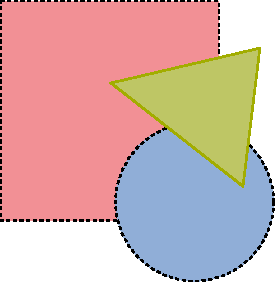
\includegraphics{shapes}

  \caption{Example Shapes from an SVG.}
  \label{fig:example_svg}
\end{figure}

\lipsum[42]



\subsection{Example Source Code}

\lipsum[1]

\begin{lstlisting}[
    language = C,
    caption  = {Example Source Code},
    label    = {list:example_src}
]
#include <stdio.h>

void quick_sort (int *a, int n) {
    int i, j, p, t;
    if (n < 2)
        return;
    p = a[n / 2];
    for (i = 0, j = n - 1;; i++, j--) {
        while (a[i] < p)
            i++;
        while (p < a[j])
            j--;
        if (i >= j)
            break;
        t = a[i];
        a[i] = a[j];
        a[j] = t;
    }
    quick_sort(a, i);
    quick_sort(a + i, n - i);
}

/* main routine */
int main (void) {
    int a[] = {4, 65, 2, -31, 0, 99, 2, 83, 782, 1};
    int n = sizeof a / sizeof a[0];
    int i;
    for (i = 0; i < n; i++)
        printf("%d%s", a[i], i == n - 1 ? "\n" : " ");
    quick_sort(a, n);
    for (i = 0; i < n; i++)
        printf("%d%s", a[i], i == n - 1 ? "\n" : " ");
    return 0;
}
\end{lstlisting}



\subsection{Example Subsection}

\lipsum[1]



\subsubsection{Example SubSubSection}

\lipsum[9]



\subsubsection{Example SubSubSection}

\lipsum[10]



\chapter{Conclusion \& Outlook}
\label{chap:conclusion}

\lipsum[1-4]



%-------------------------------------------------------------------------------
% Bibliography
%-------------------------------------------------------------------------------
%\backmatter
% unsrturl-custom works only with hyperref loaded
% use other styles like unsrt when hyperref is not loaded
\bibliographystyle{unsrturl-custom}
\bibliography{bibliography}



%-------------------------------------------------------------------------------
% Appendix
%-------------------------------------------------------------------------------
\appendix
\chapter{Additional Stuff}

\lipsum[1-4]

\end{document}

%%% Local Variables:
%%% mode: latex
%%% TeX-master: t
%%% End:
